\documentclass[letterpaper,11pt]{report}

\usepackage[utf8]{inputenc}

%idioma
\usepackage[spanish]{babel}
\selectlanguage{spanish}

%formato de bibliografia y citas
\usepackage{apacite}
 
\usepackage[nottoc]{tocbibind}

\usepackage{etoc}
\usepackage{blindtext}

%Imagenes
\usepackage{graphicx}
\graphicspath{{./images/}}
\setlength{\abovecaptionskip}{15pt plus 3pt minus 2pt}

%Espacio de interlineado
\usepackage{setspace}
\thispagestyle{empty}
\doublespacing

%Tamaño de márgenes
\usepackage[left=1.25in, right=1.25in]{geometry}

%Colores en el texto
\usepackage{xcolor}

%\setcounter{secnumdepth}{3}
%\setcounter{tocdepth}{4}

\begin{document}


\begin{center}
\begin{Large}
Universidad Nacional Autónoma de México\\
Facultad de Ciencias\\
\end{Large}
\begin{LARGE}
Proyecto para la Opción de Titulación por Reporte de Trabajo Profesional\\
AutoSAI: Sistema para automatizar las órdenes de reposición en el portal SAI del IMSS\\*[1ex]
\end{LARGE}

Alumno: Ernesto Carrillo Espinosa - No. de cuenta: 300138647\\
Tutor: M. en I. Karla Ramírez Pulido\\*[1ex]
\today
\end{center}

\clearpage
\pagenumbering{arabic}

\tableofcontents
\listoffigures
%\listoftables


\chapter{Introducción}\label{cap1}

\section{Contexto} \label{sec:intro-contexto}
Todos los institutos de salud pública en México cuentan con proveedores que se encargan de surtir los medicamentos a sus respectivas clínicas y hospitales. El documento digital en el cual se asienta la solicitud de un medicamento es llamada \textit{orden de reposición}; este documento contiene la descripción del medicamento y el lugar en donde es solicitada la entrega del mismo. En particular, el \textit{Instituto} para el cual se realiza este proyecto hace llegar a los proveedores las órdenes de reposición a través de su sistema web llamado \textit{Sistema de Abastecimiento}, dentro del cual el proveedor, a su vez, puede confirmar la recepción de las órdenes de reposición.\\
El proveedor tiene operadores dedicados a interactuar con el \textit{Sistema de Abastecimiento}. Las tareas que debe cumplir el operador del \textit{Sistema de Abastecimiento} son: confirmar la recepción de órdenes de reposición al \textit{Sistema de Abastecimiento}, obtener la información necesaria para cumplir con la entrega del medicamento (Figura \ref{fig:flow-proc-contestar}) y extraer las órdenes de reposición que han sido canceladas (Figura \ref{fig:flow-proc-verificar}), lo cual significa que el \textit{Instituto} ya no requiere el medicamento especificado en la orden de reposición y, de ser entregadas, serán rechazadas.\\
El proveedor realiza dos tipos de procesos:
\begin{enumerate}
\item \textbf{Envío de órdenes de reposición}. Un operador accede al \textit{Sistema de Abastecimiento}, con un usuario y contraseña previamente asignados, posteriormente se dirige a la sección \textit{Contestación a Órdenes de Reposición}, que es donde se muestra un listado con las órdenes de reposición emitidas por el \textit{Instituto} que aún no han sido atendidas. El operador manualmente ingresa en cada orden de reposición los datos requeridos: la cantidad de unidades que enviará, fechas de fabricación y de caducidad. A esto se le conoce como responder la orden reposición.\\
Cuando una orden de reposición ha sido \textit{contestada}, en el listado de órdenes de reposición de la sección \textit{Contestación a Órdenes de Reposición} se muestra la opción de ``enviar''. Aquí el operador selecciona la opción ``enviar'' de cada una de las órdenes de reposición que ha contestado, el \textit{Sistema de Abastecimiento} muestra el formato de acuse de recibo, el operador extrae los datos de interés que se muestran en el acuse y hace una impresión de la pantalla. El flujo descrito anteriormente se muestra en la Figura \ref{fig:flow-proc-contestar}.

\begin{figure}[H]
\centering
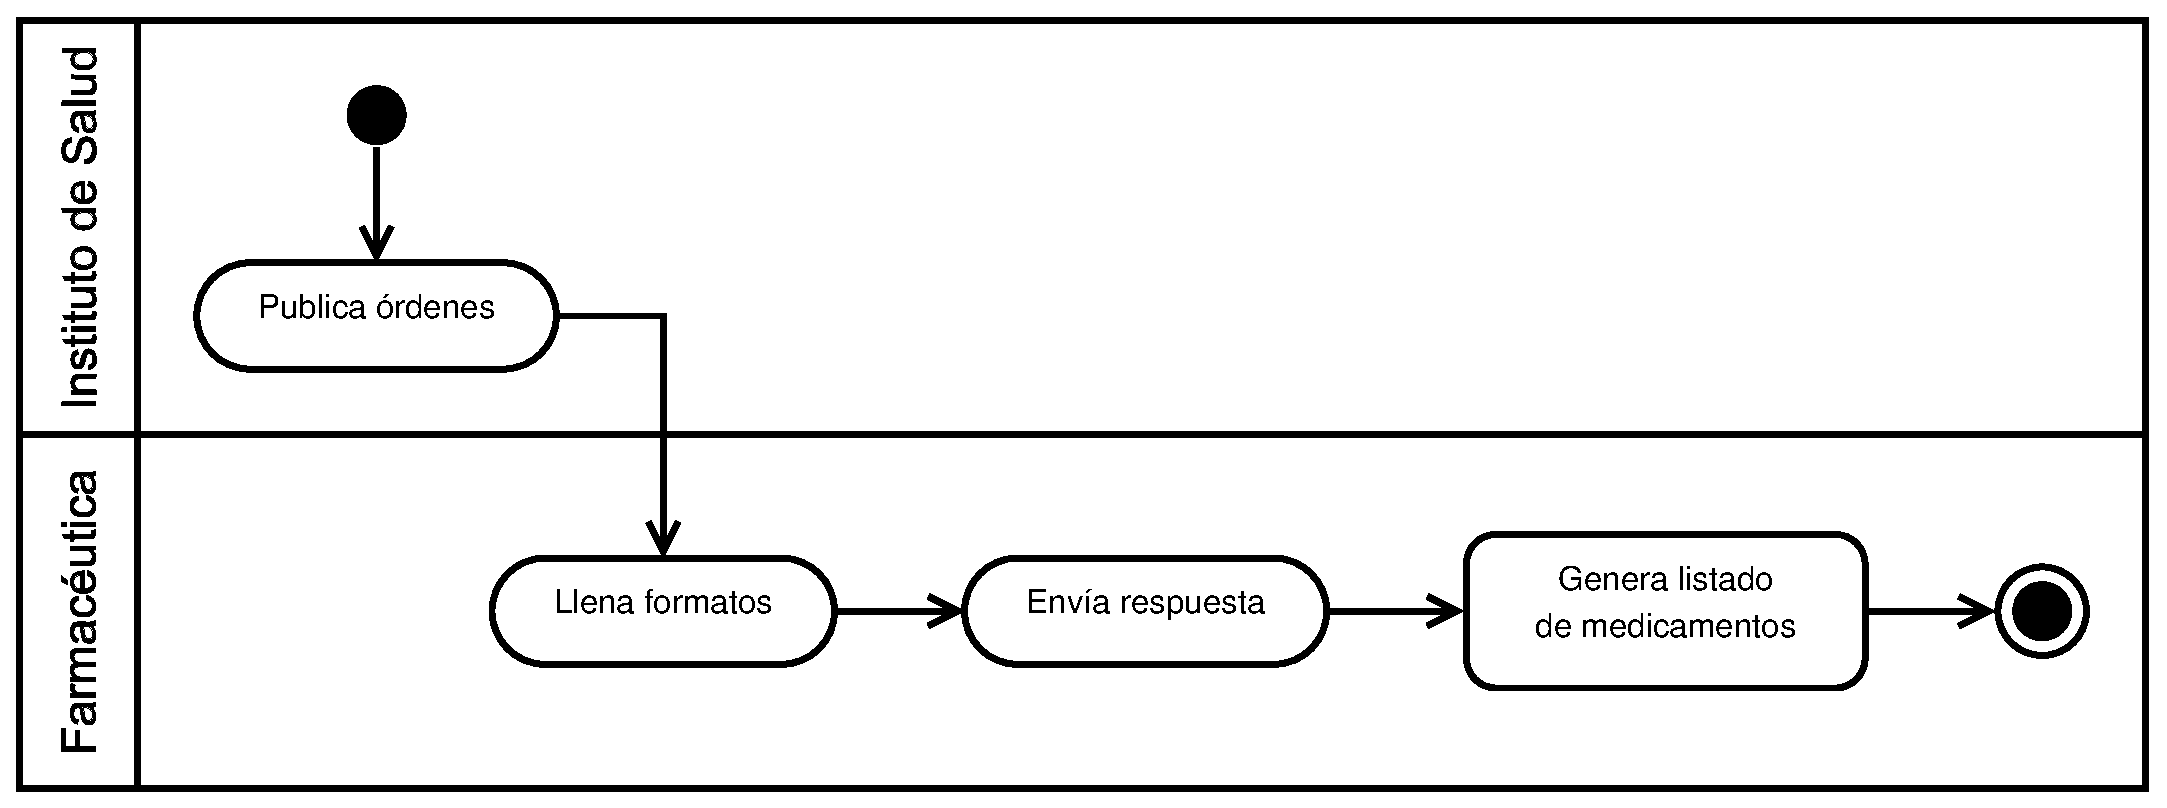
\includegraphics[scale=0.3]{flow-proc-contestar} 
\caption{Flujo del proceso para contestar órdenes de reposición.}
\label{fig:flow-proc-contestar}
\end{figure}

\item \textbf{Verificación de órdenes de reposición canceladas}. Dado que el \textit{Instituto} tiene la facultad de cancelar las órdenes aun cuando ya hayan sido enviadas, es importante para el proveedor evitar el gasto extra que implica retirar medicamento no solicitado que ya ha sido enviado al \textit{Instituto}. El operador accede al \textit{Sistema de Abastecimiento} de la misma manera como se describe en el punto anterior, se dirige a la sección \textit{Consulta de Órdenes}, donde provee información para realizar la búsqueda: rango de fechas de emisión\footnote{Fecha en que la orden fue realizada.}, el estado de la orden como ``cancelada''. Como resultado de esta búsqueda, se muestra un listado con las órdenes que cumplen con tal filtro. El operador copia la lista en un documento en su equipo personal, para posteriormente extraer las órdenes de reposición que han sido canceladas de las cuales no se tenía conocimiento. En la Figura \ref{fig:flow-proc-verificar} se muestra el proceso para verificar las órdenes de reposición canceladas.
\begin{figure}[H]
\centering
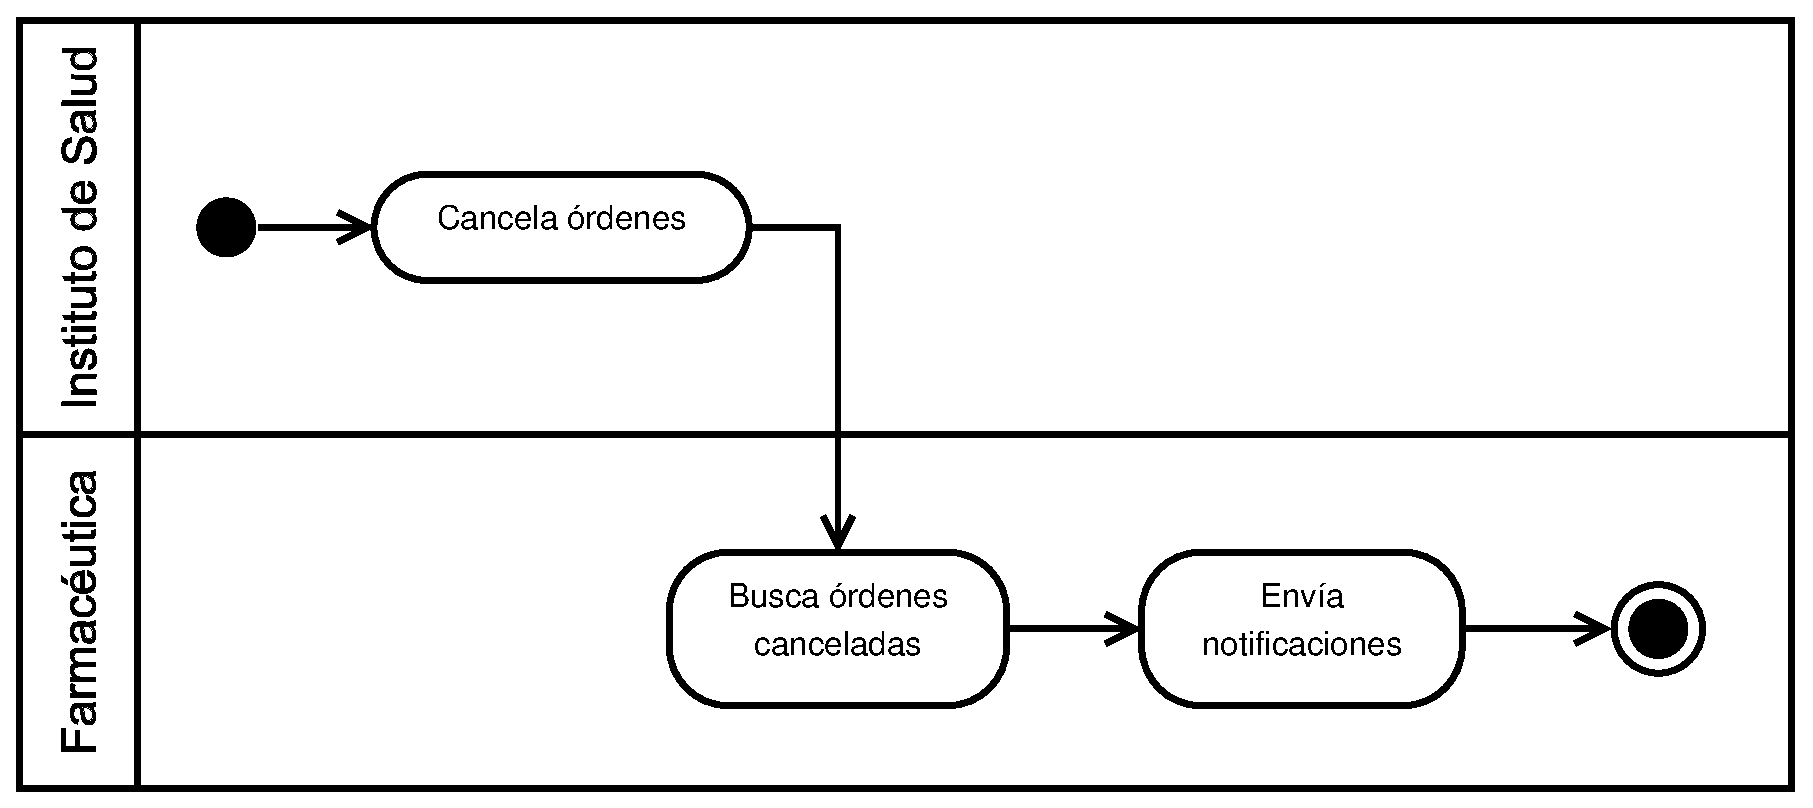
\includegraphics[scale=0.3]{flow-proc-verificar} 
\caption{Flujo del proceso para verificar órdenes de reposición canceladas.}
\label{fig:flow-proc-verificar}
\end{figure}
\end{enumerate}

En este documento se hará referencia de manera indistinta al proveedor\footnote{Quien requiere automatizar la interacción con el Sistema de Abastecimiento para el envío de las órdenes de reposición y la verificación de órdenes canceladas.} como la compañía farmacéutica o simplemente como farmacéutica.\\
Para completar las tareas de envío de órdenes de reposición y verificar las órdenes de reposición canceladas dentro del \textit{Sistema de Abastecimiento}, la farmacéutica dedica diariamente un equipo constituido por tres personas durante toda la jornada laboral. Dependiendo del volumen de órdenes de reposición emitidas por el \textit{Instituto} se puede agregar una persona más al equipo.

\section{Objetivos}
\subsection{Objetivo principal}\label{sec:objetivo-principal}
Describir un sistema de cómputo --de ahora en adelante llamado \textbf{AutoSA}-- que reduzca el tiempo de interacción entre los operadores de la farmacéutica y el \textit{Sistema de Abastecimiento}. Es así que el sistema AutoSA busca cumplir las siguientes metas:
\begin{enumerate}
	\item Reducir el tiempo utilizado para contestar las órdenes de reposición.
	\item Evitar el envío de medicamentos cuyas órdenes de reposición hayan sido canceladas.
	\item Agilizar la generación de reportes sobre las órdenes de reposición atendidas.
\end{enumerate}

\subsection{Objetivos secundarios}\label{sec:objetivos-secundarios}
\begin{enumerate}
\item Reducir el error humano en relación con la manipulación de la información.
\item Ahorrar recursos en la entrega de medicamentos no solicitados.
\item Reducir el tiempo de respuesta a las órdenes de reposición.
\item Dar consistencia en los datos respecto a la generación de reportes estadísticos sobre las órdenes de reposición procesadas.
\end{enumerate}
Por lo anterior, los afiliados del \textit{Instituto} se verán beneficiados pues los medicamentos estarán disponibles con mayor frecuencia en las clínicas y hospitales.

\section{Descripción general de trabajo}\label{sec:desc-general}
La farmacéutica atiende las órdenes de reposición del \textit{Instituto} en el doble de tiempo que su competencia, en particular contestar estas órdenes en el \textit{Sistema de Abastecimiento} requiere diariamente de tres personas dedicadas durante toda la jornada laboral para terminar esta parte del proceso. La solución propuesta para acelerar la respuesta y verificación de órdenes de reposición del \textit{Sistema de Abastecimiento} se encuentra programado por agentes\footnote{Agente dentro de este trabajo se refiere a las rutinas que automatizan los procesos realizados por los operadores del \textit{Sistema de Abastecimiento}.}. Cada agente se dedica a emular las acciones del operador de la farmacéutica, el cual es el responsable de contestar o verificar las órdenes de reposición. El sistema AutoSA cuenta con una base de datos donde se almacenan los datos capturados por los agentes durante la respuesta de órdenes y una interfaz gráfica donde los trabajadores de la farmacéutica puedan realizar tareas de administración. Estas tareas pueden ser: la búsqueda, la edición de órdenes de reposición y la generación de reportes de las órdenes atendidas por los agentes.\\
La automatización de los procesos (Figuras \ref{fig:flow-proc-contestar} y \ref{fig:flow-proc-verificar}) antes mencionados pronostica una reducción de costos por devolución de medicamento no solicitado para el cliente y también la disminución de pérdidas en las ventas por solicitudes no atendidas en los rangos de tiempo acordados con el comprador. Dado lo anterior, se plantea un proyecto de software que cubra las necesidades de automatización y pueda ser administrado por usuarios no especializados en computación.\\
Para resolver el desarrollo del proyecto, el sistema AutoSA se divide en módulos con funcionalidades específicas que se muestran a continuación:
% espaciado
%\pagebreak
% espaciado
\begin{enumerate}
\item \textbf{Automatización de interacción con el Sistema de Abastecimiento}. La automatización de la interacción con el \textit{Sistema de Abastecimiento} consiste en replicar los pasos que sigue el operador de la farmacéutica en el llenado y extracción de información de las órdenes de reposición del \textit{Sistema de Abastecimiento}, es decir, listar los pasos que sigue el operador cuando contesta las órdenes de reposición; describir las reglas de negocio necesarios para llenar los formularios que presenta el \textit{Sistema de Abastecimiento} al responder una orden de reposición; por último, se identifican las fuentes de los datos que se ocupan para llenar tales formularios y se define la forma de almacenamiento de la información necesaria de cada formulario.
\item \textbf{Generación de reportes}. La generación de reportes consiste en plasmar la información obtenida de las órdenes de reposición contestadas en el módulo anterior. La farmacéutica tiene ya una plantilla que se utiliza para pasar los pedidos a otras áreas, con el fin de continuar la atención de las órdenes de reposición; además de obtener estadísticas relacionadas con la cantidad de órdenes de reposición atendidas y canceladas.
\item \textbf{Interfaz de usuario}. La interfaz de usuario se refiere a la aplicación que muestra una interfaz gráfica en la cual los operadores de la farmacéutica pueden solicitar la generación de reportes, hacer consultas y modificaciones a las órdenes de reposición atendidas por el primer módulo.
\end{enumerate}

\subsection{Arquitectura de la solución}
Una definición de arquitectura de software es dada por Bourque\cite{SWEBOOK}:
\begin{quote}
El conjunto de estructuras necesarias para la comprensión de un sistema en el cual se comprometen elementos de software, relaciones entre ellos y sus propiedades.
\end{quote}
Esta definición expone que los requerimientos del cliente se traducen en especificaciones técnicas para los desarrolladores. Aplicando la definición anterior al presente proyecto donde tenemos los siguientes componentes (Figura \ref{fig:dia-package-small}):
\begin{figure}[h]
\centering
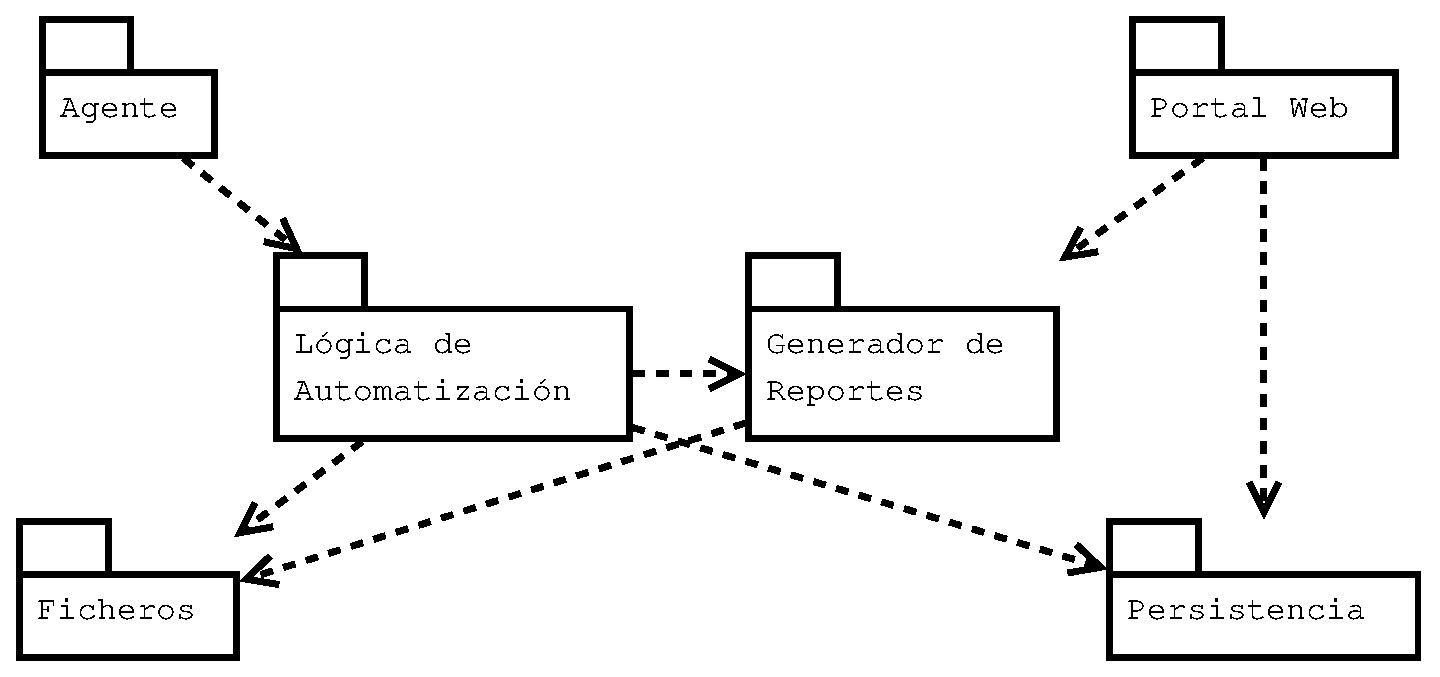
\includegraphics[scale=0.5]{dia-package-small} 
\caption{Módulos de la arquitectura.}
\label{fig:dia-package-small}
\end{figure}
% espaciado
%\pagebreak
% espaciado
\begin{itemize}
\item \textbf{Agente (robot)}. Interactúa directamente con el \textit{Sistema de Abastecimiento}, es el componente que automatiza las acciones de los operadores humanos de la farmacéutica.
\item \textbf{Lógica de Automatización}. Son bibliotecas y rutinas que se encargan de prestar los servicios necesarios al agente para su funcionamiento. Permite comunicación con la base de datos, guarda las capturas de pantalla en el sistema de archivos y provee la configuración de inicio al agente.
\item \textbf{Persistencia}. Es el componente que se encarga de llevar la persistencia de los datos obtenidos durante la respuesta a las órdenes de reposición.
\item \textbf{Ficheros}. Este componente es el encargado de manejar operaciones con el sistema de archivos para almacenar las capturas de pantalla al momento de enviar la respuesta de cada orden de reposición.
\item \textbf{Generador de Reportes}. Este módulo está encargado de la generación de reportes, tales como: órdenes de reposición atendidas, canceladas y formatos de órdenes de reposición enviadas.
\item \textbf{Portal Web}. Portal mediante el cual los usuarios pueden hacer correcciones a los datos obtenidos de las órdenes de reposición, reimprimir el formato de envío de la orden de reposición  y descargar los reportes generados por el módulo generador de reportes.
\end{itemize}
% espaciado
%\pagebreak
% espaciado
\subsection{Metodología utilizada}
El proyecto es abordado con la metodología \textit{Scrum}, la cual es un marco de trabajo para desarrollar, entregar y mantener productos complejos. Ésta consiste en un conjunto de roles, eventos, artefactos y reglas que los ligan. \textit{Scrum} da un enfoque adaptivo mientras promueve la entrega continua de soluciones y divide el desarrollo en ventanas de tiempo llamadas \textit{sprint}\cite{scrum}.\\
Dentro de \textit{Scrum} destacan los siguientes roles utilizados para el desarrollo del proyecto AutoSA\cite{scrum}:
\begin{itemize}
	\item \textit{Product Owner}: es responsable de maximizar el valor del producto que resulta del trabajo del \textit{Development Team}. Es la persona encargada de mantener el conjunto de tareas pendientes para futuros \textit{sprints}.
	\item \textit{Development Team}: es un grupo de profesionales encargado de realizar el trabajo necesario para completar las entregas de cada \textit{sprint}.
	\item \textit{Scrum Master}: es la persona responsable de promover y soportar \textit{Scrum} como está definido en la guía de \textit{Scrum}. Es un líder servil para el \textit{Scrum Team} que auxilia a este último a maximizar el valor del producto creado y ayuda a los involucrados en el desarrollo a comprender \textit{Scrum}.
	\item \textit{Scrum Team}: es conformado por el \textit{Product Owner}, el \textit{Development Team} y el \textit{Scrum Master}. \textit{Scrum Team} es un equipo de trabajo autoorganizado y multifuncional. Está diseñado para optimizar la flexibilidad, creatividad y productividad sin depender de personas ajenas al equipo.
	\item \textit{Stakeholder}: esta definición proviene directamente de su significado en inglés, refiere a las personas que tienen interés en el producto.
\end{itemize}
El grupo de trabajo (\textit{Scrum Team}) formado por la consultora para el proyecto AutoSA consta de dos personas:
\begin{enumerate}
	\item Desarrollador: es la persona que cumple con las funciones siguientes:
	\begin{enumerate}
		\item Levantar los requerimientos de los \textit{stakeholders} de la farmacéutica.
		\item Cumplir con el rol de \textit{Product Owner} al ser encargado de mantener la lista de tareas para los \textit{sprints} futuros.
		\item Hacer investigación sobre tecnologías adecuadas para el desarrollo.
		\item Realizar el diseño e implementación de los componentes del sistema AutoSA.
		\item Formar parte del \textit{Scrum Team}.
	\end{enumerate}
	\item Arquitecto: tiene las siguientes responsabilidades:
	\begin{enumerate}
		\item Supervisar y aprobar el diseño e implementación realizado por el desarrollador.
		\item Hacer investigación sobre tecnologías adecuadas para el desarrollo.
		\item Cumplir con el rol de \textit{Scrum Master}.
		\item Formar parte del \textit{Scrum Team}.
	\end{enumerate}
\end{enumerate}
El proyecto fue planeado para ser realizado de julio a diciembre de 2014. Su conclusión es la liberación del sistema AutoSA que consiste en el despliegue total de los módulos en el ambiente productivo provisto por la farmacéutica dando como resultado los siguientes productos:
\begin{itemize}
\item Rutinas para la generación de objetos en base de datos.
\item Rutinas para la creación de la estructura de directorios en el sistema de archivos.
\item Archivos de configuración propios de cada módulo.
\item Herramienta y rutinas de automatización.
\item Bibliotecas del portal web.
\item Manual de instalación y de usuario.
\item Capacitación a usuarios finales.
\end{itemize}
El autor del presente documento cumplió con rol de desarrollador desde el inicio del proyecto AutoSA hasta su liberación.

\section{Resumen}
El \textit{Instituto de Salud}, mediante su \textit{Sistema de Abastecimiento}, realiza las órdenes de reposición de medicamentos a las farmacéuticas. Estas últimas invierten veinticuatro horas hombre por día para lograr contestar todas las órdenes de reposición. Reducir el tiempo en que se contestan las órdenes de reposición aumenta la velocidad de respuesta de la farmacéutica para entregar los medicamentos a centros de salud del \textit{Instituto}, motivo por el cual le interesa automatizar esta parte. El sistema AutoSA que se propone en este documento da solución mediante dos subsistemas: uno que automatiza los procedimientos de interacción con el \textit{Sistema de Abastecimiento} y otro que permite al personal de la farmacéutica generar reportes y acceder a datos de las órdenes de reposición atendidas.
\chapter{Análisis y alcance del proyecto}\label{cap2}

En este capítulo se establecen los requerimientos que satisfacen las necesidades de la farmacéutica planteadas en al capítulo anterior, como se verá más adelante, los requerimientos se clasifican en funcionales y no funcionales, de igual forma se delimita el alcance y los riesgos del proyecto; con los elementos anteriores se redactan los casos de uso, los flujos lógicos que satisfacen los requerimientos dentro del alcance definido.
%===============================================================================
%===============================================================================


\section{Análisis de requerimientos}
En general, los requerimientos deben reflejar lo que un usuario espera de una aplicación, tales requerimientos se clasifican en requerimientos funcionales y no funcionales:
\begin{itemize}
\item \textbf{Requerimientos funcionales}: descripciones detalladas de las funciones deseadas del proyecto\cite{WileyBegSE}.
\item \textbf{Requerimientos no funcionales}: descripciones de la calidad y capacidades del comportamiento del proyecto\cite{WileyBegSE}.
\end{itemize}
Con las definiciones anteriores es posible ejemplificar sobre la funcionalidad para la generación de reportes: un requerimiento funcional necesita en general, de los datos que deben ser capturados por un usuario para obtener así un reporte (fechas de inicio y término, número de orden, etcétera), mientras que un requerimiento no funcional refleja el formato de salida, verificación de permisos de usuario para generar el reporte,  capacidad del sistema para atender generación simultánea de varios reportes.\\
Los requerimientos se ven acotados por el alcance del proyecto, es decir, las funciones que realizará el sistema para completar los procesos y funciones que son automatizadas por el sistema AutoSA\cite{WileyBegSE} (en la sección \ref{sec-alcance} se describen los procesos automatizados). De igual manera, automatizar los procesos de la farmacéutica conlleva ciertos riesgos. Uno de estos riesgos dentro de este contexto se encuentra definido como un fallo o mal funcionamiento del sistema bajo condiciones específicas y que muchas veces escapa al control del sistema.\\
Por ejemplo: la caída de el servidor de base de datos, en siguientes secciones también se formalizará el concepto de riesgo (ver sección \ref{sec-riesgos}).


\subsection{Alcance del proyecto}\label{sec-alcance}
Moustafaev define el alcance del proyecto de software como:
\begin{quote}
\textit{Es el proceso de definir todo el trabajo necesario para entregar un producto o servicio con las funciones y características especificadas\cite{ScopeManagement}.}
\end{quote}
Para fines del sistema AutoSA, el alcance está acotado en los siguientes puntos:
\begin{itemize}
\item Automatizar el proceso para contestar órdenes de reposición en Sistema de Abastecimiento.
\item Almacenamiento de los datos de las órdenes de reposición contestadas.
\item Generación del formato de salida que se realiza al terminar de responder las órdenes de reposición (ver Figura \ref{fig:flow-proc-contestar})
\item Automatizar el proceso para verificar las órdenes de reposición canceladas recientemente en Sistema de Abastecimiento.
\item Actualización de catálogos propios del sistema AutoSA que contienen claves de medicamentos y centros de salud del Instituto.
\item Actualización masiva de las órdenes de reposición que han sido canceladas y notificado al área correspondiente para detener el envío de medicamentos.
\item Queda fuera de alcance la verificación de existencia del medicamento en bodega.
\item Queda fuera de alcance la realización de respaldos de la información contenida en la base de datos o en el sistema de archivos.
\item El sistema no emitirá notificaciones de las órdenes de reposición canceladas recientemente.
\end{itemize}


\subsection{Riesgos asociados al proyecto}\label{sec-riesgos}
Moustafaev define el riesgo de un proyecto como:
\begin{quote}
Riesgo es la incertidumbre sobre escenarios que pueden arriesgar el éxito del proyecto.\cite{ScopeManagement}.
\end{quote}
Los riesgos identificados para este proyecto se listan a continuación:
\begin{enumerate}
  \item Dado que no se cuenta con un ambiente de pruebas del Sistema de Abastecimiento todos los datos alterados durante la programación de las rutinas de automatización podrían presentar información incorrecta, por lo que es necesario mantener siempre un registro de las órdenes de reposición alteradas durante el desarrollo de las rutinas de automatización.
  \item La herramienta de automatización Sahi está basada en la estructura de las páginas del sistema Sistema de Abastecimiento. Si ocurriera un cambio en dicha estructura las rutinas de automatización podrían dejar de funcionar.
  \item La herramienta Sahi en su versión libre\footnote{El uso de la versión libre de Sahi es requerido por la farmacéutica, ver sección \ref{sec:nonfunctional-req}.} no cuenta con soporte bajo demanda por lo que una falla en la herramienta durante el desarrollo del sistema podría causar retrasos en la entrega del sistema AutoSA.
\end{enumerate}


\subsection{Requerimientos funcionales}
\subsubsection{Automatización del proceso para contestar órdenes de reposición}
Automatizar la interacción del operador de la farmacéutica\footnote{Se realiza utilizando el Sistema de Abastecimiento.} para contestar las órdenes de reposición, como se muestra en el diagrama de proceso de negocio en la Figura \ref{fig:dia-activity-contestar}\footnote{Ver también la Figura \ref{fig:flow-proc-contestar}.}, esto implica almacenar los datos de las órdenes de reposición, los cuales son utilizados para generar el formato de salida que es entregado al almacén para continuar con la atención de las órdenes.

\begin{figure}[h]
  \centering
  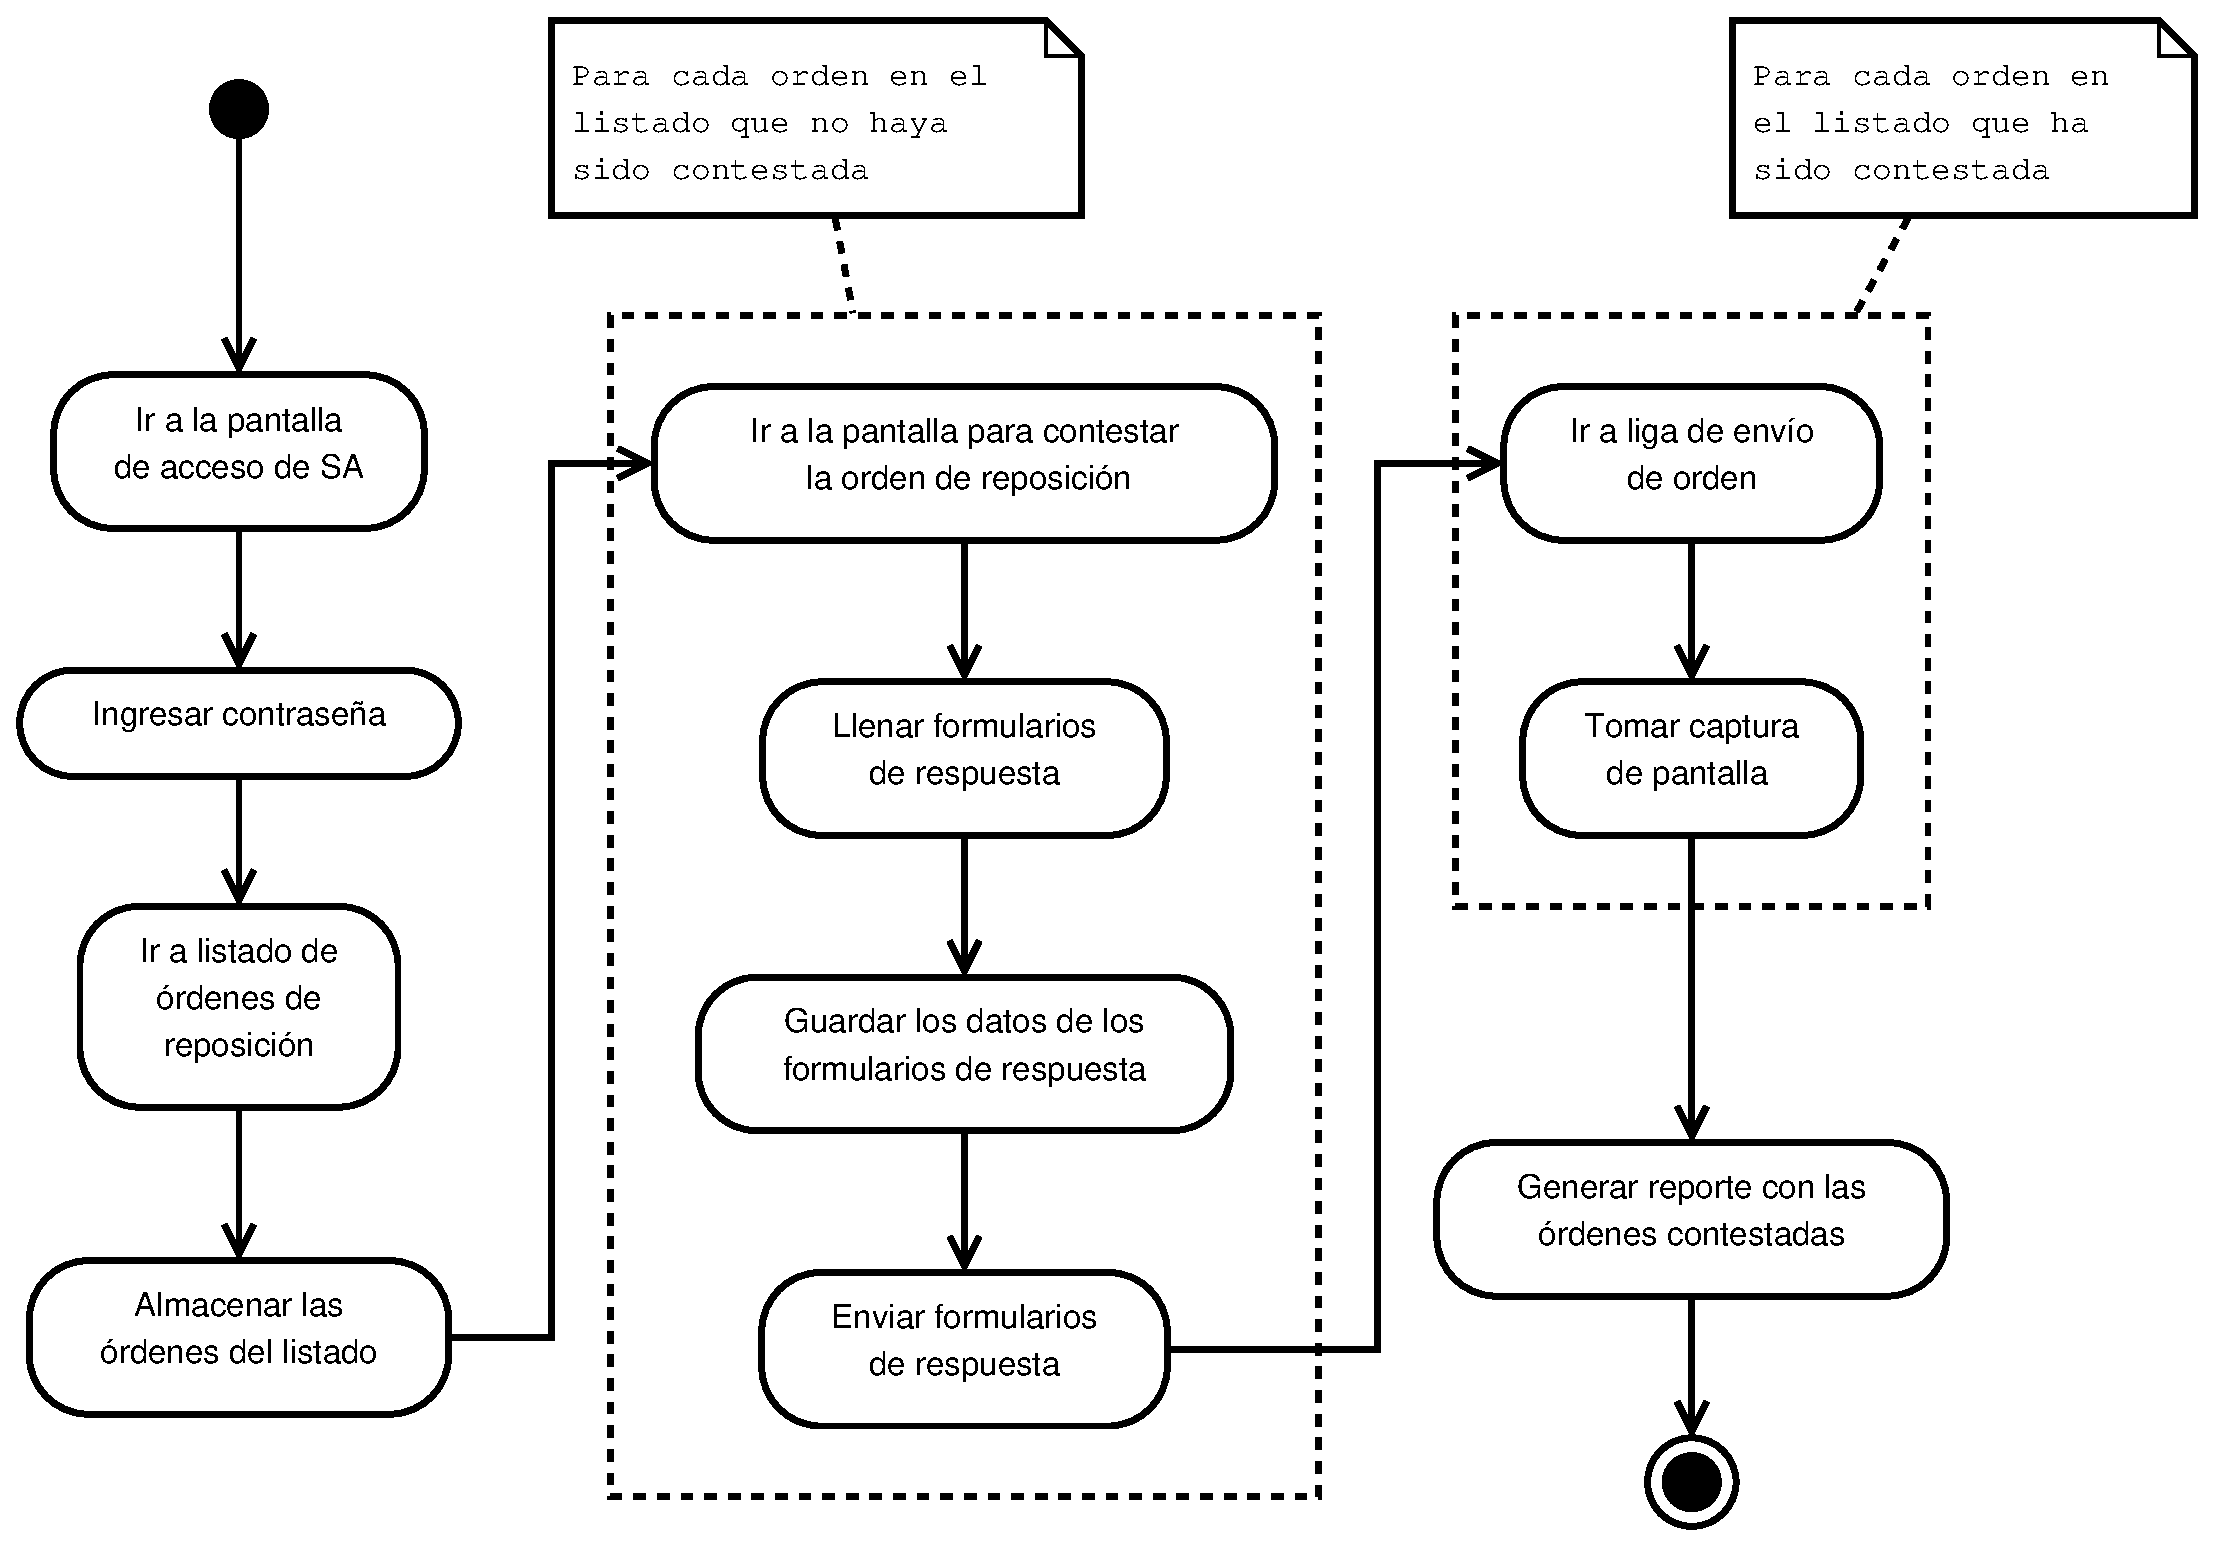
\includegraphics[scale=0.4]{dia-activity-contestar}
  \caption{Diagrama de proceso de negocio que sigue un operador de la farmacéutica para contestar órdenes de reposición.}
  \label{fig:dia-activity-contestar}
\end{figure}

\subsubsection{Automatización del proceso para cotejar órdenes de reposición canceladas}
Automatizar la interacción del operador de la farmacéutica para conocer las órdenes de reposición que han sido canceladas recientemente por el Instituto, como se muestra en el diagrama de proceso de negocio en la Figura \ref{fig:dia-activity-verificar} \footnote{
Ver también la Figura \ref{fig:flow-proc-verificar}.}.
\begin{figure}[h]
  \centering
  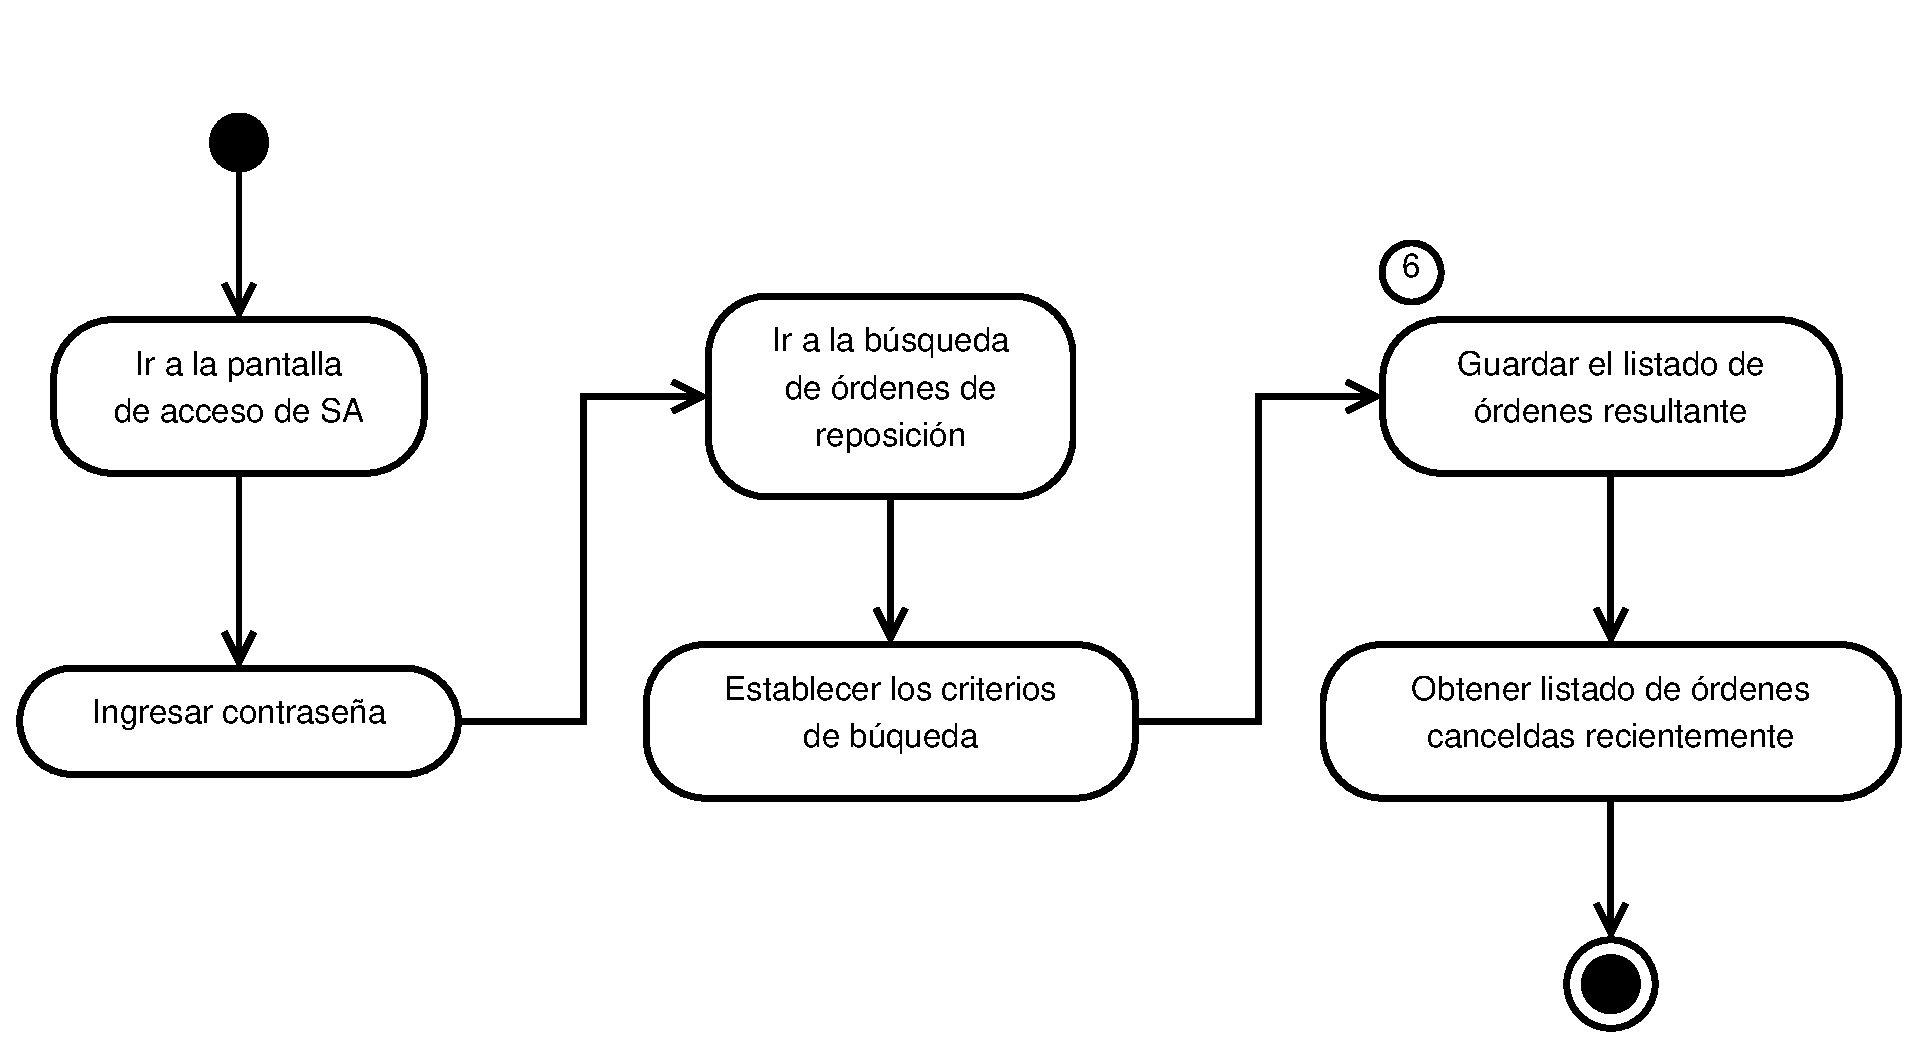
\includegraphics[scale=0.4]{dia-activity-verificar}
  \caption{Diagrama de proceso de negocio que sigue un operador de la farmacéutica para verificar órdenes de reposición canceladas.}
  \label{fig:dia-activity-verificar}
\end{figure}

\subsubsection{Interfaz WEB para la administración de órdenes de reposición contestadas}
Todos los requerimientos de administración de órdenes de reposición y generación de reportes deben ser accedidos mediante una interfaz web protegida por nombre de usuario y contraseña\footnote{Excepto lo referente a los procesos automatizados de los operadores de la farmacéutica.}, como se muestra en la Figura \ref{fig:maq-login}.
\begin{figure}[h]
  \centering
  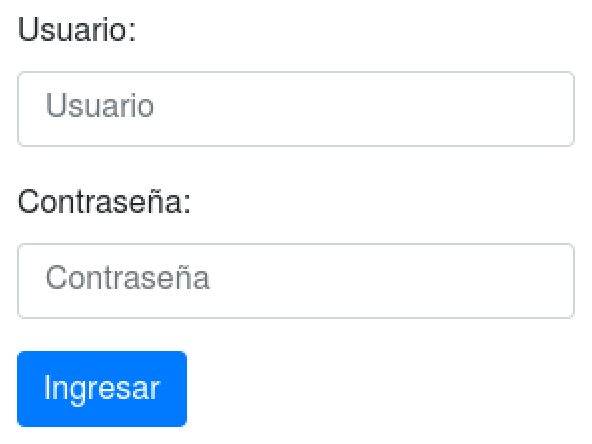
\includegraphics[scale=0.5]{maq-login} 
  \caption{Maqueta del acceso a la interfaz web.}
  \label{fig:maq-login}
\end{figure} 

\subsubsection{Búsqueda de órdenes de reposición}
En la interfaz web existe la posibilidad de buscar entre las órdenes de reposición contestadas mediante el número de orden de reposición. Esta opción entrega solo una orden de reposición, o bien se puede utilizar un intervalo de fechas entre las cuales fueron atendidas tales órdenes, entregando un listado de todas las órdenes de reposición que fueron respondidas en dicho intervalo. Las órdenes resultantes de la búsqueda deben ofrecer la opción para visualizar la información almacenada durante el proceso de respuesta, como se muestra en la Figura \ref{fig:maq-search}
\begin{figure}[h]
  \centering
  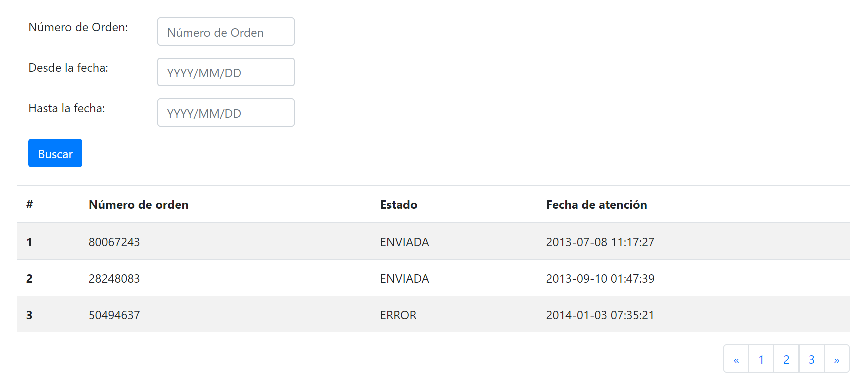
\includegraphics[width=\textwidth]{maq-search} 
  \caption{Maqueta de la búsqueda de órdenes.}
  \label{fig:maq-search}
\end{figure} 

\subsubsection{Visualización de orden de reposición}
La interfaz WEB tiene una sección donde se muestra el contenido de una orden de reposición almacenada en la base de datos (ver Figura \ref{fig:maq-crud}), esta vista es individual, (no es posible mostrar el contenido de más de una orden de reposición), además ofrece las opciones para modificar los datos de la orden (ver requerimiento \ref{req-edicion}) y para generar el acuse de envío.
\begin{figure}[h]
  \centering
  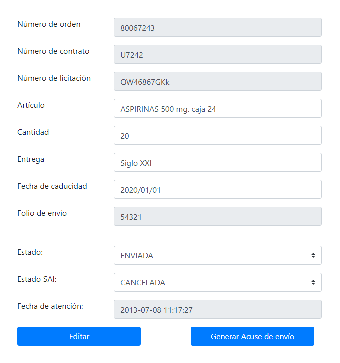
\includegraphics[scale=1]{maq-crud} 
  \caption{Maqueta del formulario para ver la información de una orden de reposición.}
  \label{fig:maq-crud}
\end{figure} 

\subsubsection{Edición de órdenes de reposición}\label{req-edicion}
La interfaz web cuenta con una vista (similar a la forma de mostrar la información de una orden de reposición) que permite la modificación de una orden de reposición (ver Figura \ref{fig:maq-crud}), esta vista es única (no es posible modificar más de una orden de reposición), por lo que no es posible modificar datos el número de orden y fecha de atención.

\subsubsection{Generación de reporte de órdenes de reposición contestadas}
El reporte con órdenes de reposición contestadas es acotado entre un par de fechas (con precisión de horas), tal reporte (ver Figura \ref{fig:maq-report}), como su nombre lo indica, contiene los números de orden de reposición y datos definidos por la farmacéutica\footnote{Por acuerdo de confidencialidad no se enunciarán los datos contenidos en los reportes.}
\begin{figure}[h]
  \centering
  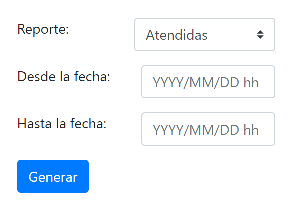
\includegraphics[scale=1.2]{maq-report} 
  \caption{Maqueta de la generación de reportes.}
  \label{fig:maq-report}
\end{figure} 

\subsubsection{Generación de formato de salida}
Este formato contiene los datos de las órdenes de reposición, las claves de los productos, como los nombres de los centros de salud. El reporte (ver Figura \ref{fig:maq-report})\footnote{Por acuerdo de confidencialidad no se enunciarán los datos contenidos en el formato de salida así como el contenido de los catálogos de claves de producto y centros de salud.} está acotado entre un par de fechas (con precisión de horas).

\subsubsection{Generación de reporte con las órdenes de reposición canceladas recientemente}
Genera un reporte con las órdenes de reposición canceladas recientemente (ver Figura \ref{fig:maq-report}), es decir, las órdenes de reposición que tienen el estado de “cancelada” y no se han marcado como canceladas en el proceso de respuesta.

\subsubsection{Actualización de catálogos}
Cargar de forma masiva, mediante un archivo separado por comas (ver Figura \ref{fig:maq-upload}), los catálogos con claves de medicamentos, centros de salud y claves propias del manejo de la farmacéutica. Los catálogos definidos para la operación del sistema AutoSA no podrán ser actualizados, por ejemplo, los catálogos que contienen los estados posibles de una orden de reposición cuando dentro del flujo de atención (ver Figura \ref{fig:dia-estados-orden}).
\begin{figure}[h]
  \centering
  
\includegraphics[scale=1.3]{maq-upload}
  \caption{Maqueta para la actualización de catálogos}
  \label{fig:maq-upload}
\end{figure}

\subsubsection{Actualización de estatus de órdenes de reposición canceladas}
Para realizar la actualización del estatus de las órdenes de reposición canceladas, el usuario carga al sistema un archivo de texto separado por comas, similar a la actualización de catálogos (ver Figura \ref{fig:dia-estados-orden}), con los números de las órdenes de reposición que han sido canceladas y se ha notificado al área correspondiente de la farmacéutica para cancelar la atención de dichas órdenes.

\subsection{Navegación dentro de la interfaz web}
La interfaz web muestra en todo momento un menú que permite la navegación entre las siguientes secciones (ver Figura \ref{fig:dia-nav-flow}):
\begin{enumerate}
  \item Generación de reportes.
  \item Actualización de catálogos (incluye la actualización de órdenes canceladas).
  \item Búsqueda de órdenes de reposición.
\end{enumerate}
\begin{figure}[h]
  \centering
  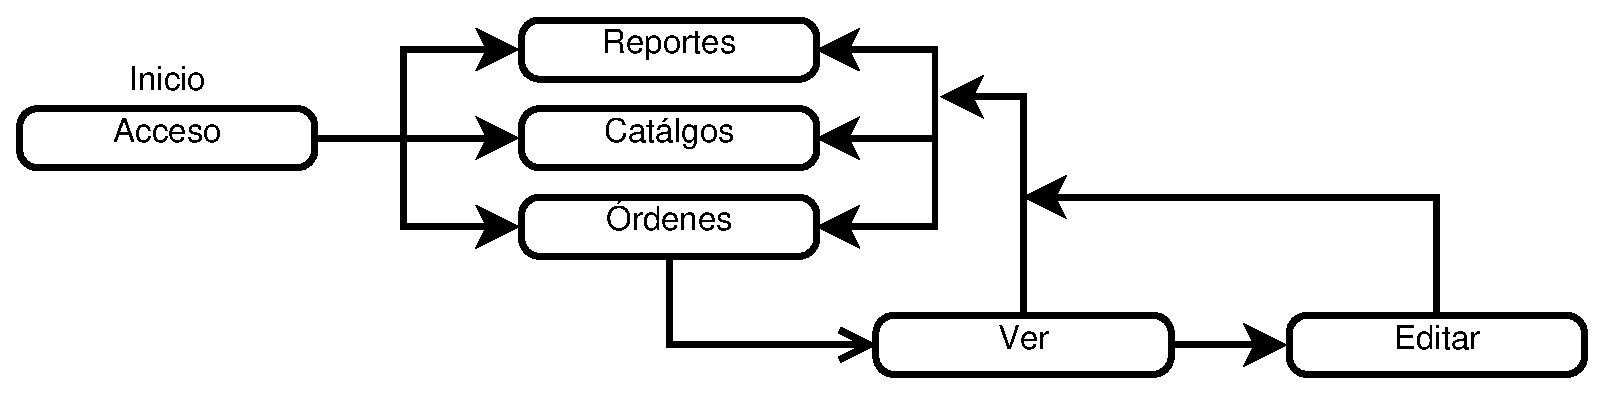
\includegraphics[scale=0.5]{dia-nav-flow}
  \caption{Mapa de navegación en la interfaz Web}
  \label{fig:dia-nav-flow}
\end{figure}


\subsection{Requerimientos no funcionales}\label{sec:nonfunctional-req}
El cliente ha solicitado que el proyecto se apegue a su infraestructura, para conservar el acuerdo de confidencialidad y evitar exponer al cliente a riesgos de seguridad informática por lo que el sistema debe de contar con\footnote{Por políticas de seguridad de la farmacéutica no se enunciarán las herramientas e infraestructura utilizada, así como las versiones de las mismas.}:
\begin{enumerate}
\item Sistema operativo capaz de ejecutar el software Java Virtual Machine (JVM).
\item Base de datos relacional SQL.
\item Uso de la herramienta Sahi para automatizar interacción con Sistema de Abastecimiento.
\item Las contraseñas de los usuarios para el acceso a la interfaz web deben ser almacenadas utilizando un algoritmo de cifrado.
\end{enumerate}


%===============================================================================
%===============================================================================


\section{Casos de uso}\label{sec:casos-uso}
Un caso de uso es la representación de las posibles interacciones entre el sistema y sus actores, entendiendo un actor como una instancia (usuario u otro sistema). Así mismo, un caso de uso describe la funcionalidad del sistema por medio de mensajes y respuestas entre el actor y el sistema\cite{ApressSE}. A continuación se muestra el diagrama de casos de uso del sistema AutoSA.

\begin{figure}[h]
  \centering
  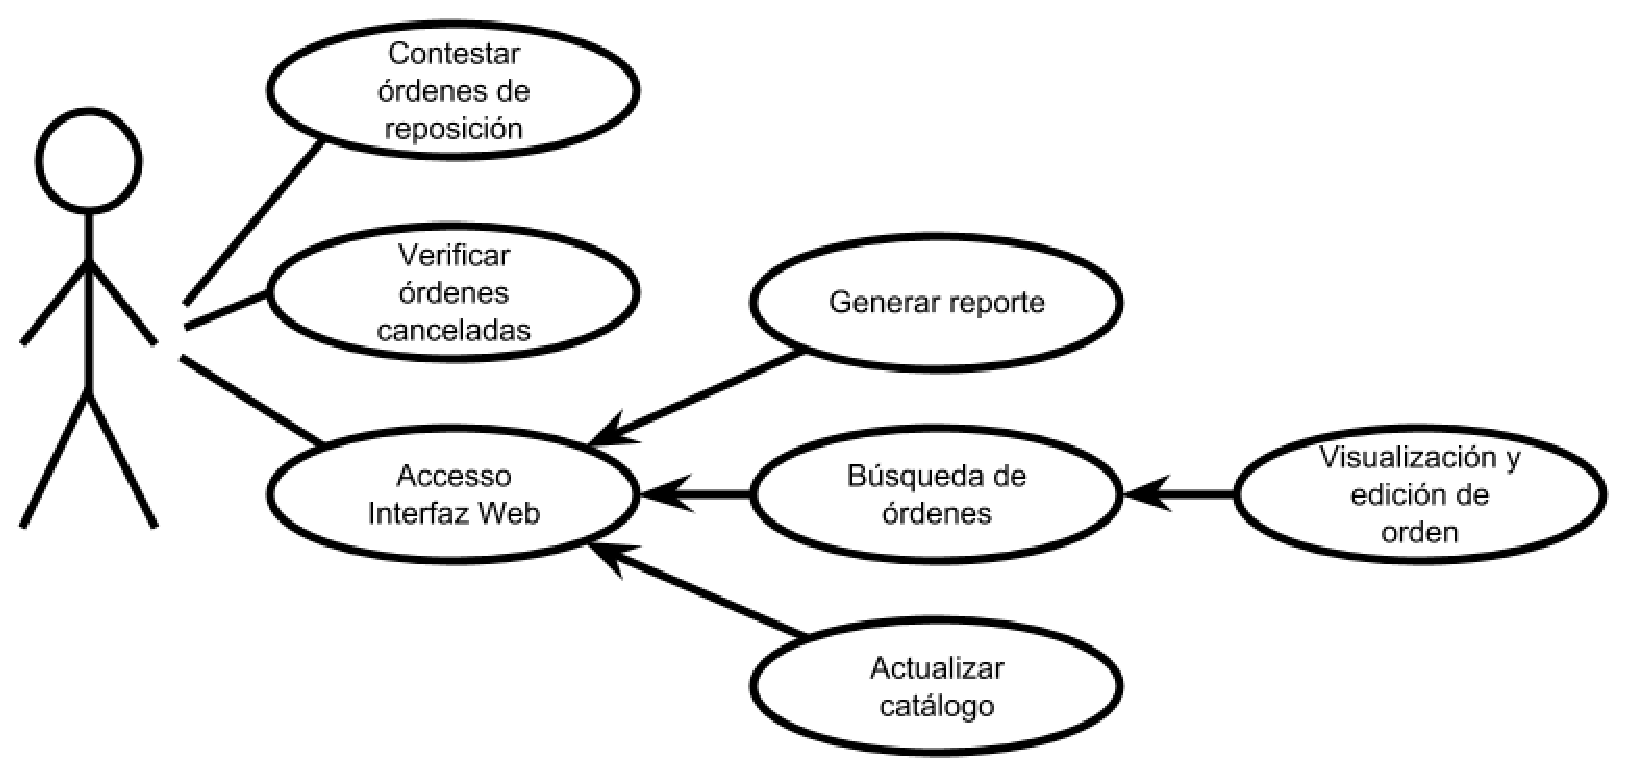
\includegraphics[width=\textwidth]{dia-casos-uso} 
  \caption{Diagrama de casos de uso.}
  \label{fig:dia-casos-uso}
\end{figure}

Con el fin de explicar mejor el flujo de atención de una orden de reposición es necesario mostrar el diagrama de estados de una orden de reposición durante el flujo de \textbf{envío de órdenes de reposición} (ver sección \ref{sec:intro-contexto}).\\
Los estados que puede tomar una orden (ver Figura \ref{fig:dia-estados-orden}) indican:
\begin{itemize}
  \item Si la solicitud está lista para ser procesada: ``Nueva'' o ``Contestada''.
  \item Si está siendo procesada: ``Siendo Contestada'' o ``Siendo Enviada''.
  \item Si ha terminado el ciclo correctamente: ``Enviada''.
  \item Si ha terminado el ciclo con errores: ``Error''.
\end{itemize} 

\begin{figure}[h]
  \centering
  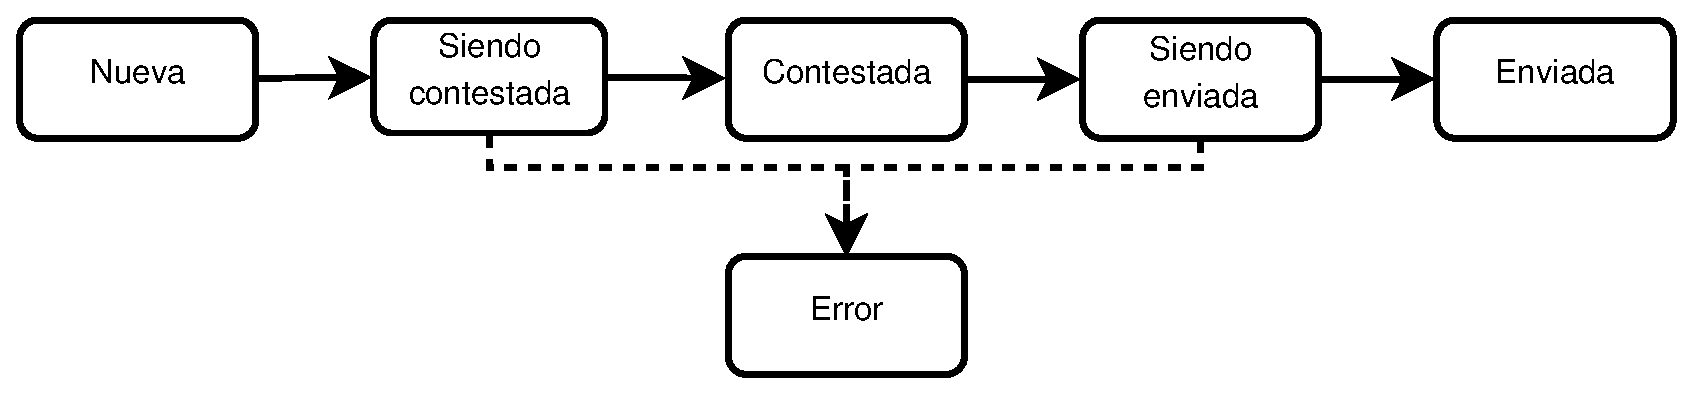
\includegraphics[width=\textwidth]{dia-estados-orden} 
  \caption{Diagrama de estados de una orden de reposición durante la ruta de respuesta de órdenes de reposición.}
  \label{fig:dia-estados-orden}
\end{figure}

Es importante mencionar que en las siguientes descripciones de caso de uso no se hará referencia al contenido exacto de las páginas así como el nombre de los campos, únicamente se hará mención de los campos necesarios para dar una explicación clara del caso.

\subsection{Contestar órdenes}\label{cu-contestar}
\paragraph{Identificador:}
CU-CONTESTAR
\paragraph{Actores:}
Usuario
\paragraph{Descripción:}
El procedimiento completo para contestar las órdenes de reposición listadas en el Sistema de Abastecimiento del Instituto (ver Figura \ref{fig:dia-activity-contestar}), el alcance de este caso comprende el acceso al Sistema de Abastecimiento, contestar y enviar las órdenes de reproducción almacenando los datos y generando la captura de pantalla de dichas órdenes.\\
Queda fuera de alcance la obtención del reporte con las órdenes de reposición que han sido canceladas recientemente es cubierto por el caso de uso Generación de Reportes.
\paragraph{Precondiciones:}
\begin{enumerate}
  \item El Sistema de Abastecimiento se encuentra funcionando correctamente.
  \item El usuario cuenta con las credenciales para ingresar al Sistema de Abastecimiento.
\end{enumerate}
\paragraph{Secuencia normal:}
\begin{enumerate}
  \item Inicia sesión en Sistema de Abastecimiento: provee nombre de usuario y le solicita al usuario ingresar la contraseña.
  \item Dirige el explorador a la pantalla donde se encuentra el listado con las órdenes de reposición que no han sido contestadas.
  \item Para cada orden de reposición del listado que se muestra se aplica el caso de uso CU-GUARDAR-NUEVA.
  \item Para cada solicitud en la base de datos con estado \textbf{Nueva} se aplican los casos de uso:
  \begin{enumerate}
    \item CU-RESPONDER-ORDEN.
  \end{enumerate}
  \item Para cada solicitud con estatus \textbf{Contestada}:
  \begin{enumerate}
    \item CU-ENVIAR-ORDEN
    \item CU-GENERAR-ACUSE
  \end{enumerate}
  \item El programa se repite desde el paso 2 hasta terminar las solicitudes sin contar las marcadas con estatus \textbf{Error}.
  \item Registra el fin del procedimiento en la base de datos.
\end{enumerate}
\paragraph{Postcondiciones:}
\begin{enumerate}
  \item Todas las órdenes de reposición listadas han sido contestadas y enviadas.
  \item Se han registrado todas las órdenes de reposición atendidas en la base de datos.
  \item Los acuses de envió de las órdenes de reposición se encuentran en el sistema de archivos.
\end{enumerate}
\paragraph{Excepciones:}
\begin{enumerate}
  \item Si en algún momento se detecta la pérdida de sesión en la página Sistema de Abastecimiento, se reinicia el procedimiento desde el paso 1 de este caso de uso.
  \item Cualquier error durante la ejecución de este caso de uso será registrado en la bitácora el sistema.
\end{enumerate}


\subsection{Guardar nueva orden}\label{cu-guardar-nueva}
\paragraph{Identificador:}
CU-GUARDAR-NUEVA
\paragraph{Actores:}
Robot
\paragraph{Descripción:}
Una orden de reposición es almacenada por primera vez con la información que se muestra en el listado de órdenes de reposición.
\paragraph{Precondiciones:}
\begin{enumerate}
  \item Se tiene indicado un renglón del listado de órdenes de reposición sobre el cuál se realizará este caso de uso.
\end{enumerate}
\paragraph{Secuencia normal:}
\begin{enumerate}
  \item Del listado de órdenes de reposición, cada solicitud es ingresada a la base de datos con estatus \textbf{Nueva} y datos provenientes del listado:
  \begin{enumerate}
    \item Contrato.
    \item Solicitud.
    \item Número de orden.
    \item Fecha de expedición.
    \item Almacén destino.
    \item \textit{URL} de respuesta.
    \item \textit{URL} de envío: generada reemplazando el parámetro en la \textit{URL} de respuesta ``responde'' por ``envia''\footnote{Dado que es una palabra en una URL no es recomendable el uso de acentos, por lo tanto se escribe \textbf{envia} y no \textbf{envía}.}.
  \end{enumerate}
\end{enumerate}
\paragraph{Postcondiciones:}
\begin{enumerate}
  \item La orden de reposición se encuentra almacenada en la base de datos.
\end{enumerate}
\paragraph{Excepciones:}
\begin{enumerate}
  \item Si el listado muestra la URL de envío y la orden no ha sido almacenada, entonces la orden es almacenada con estado \textbf{Contestada} y se registra la \textbf{cantidad solicitada} en 0.
  \item Si ocurre algún error la orden es almacenada con estado \textbf{Error}.
\end{enumerate}


\subsection{Responder orden}\label{cu-responder-orden}
\paragraph{Identificador:}
CU-RESPONDER-ORDEN
\paragraph{Actores:}
Robot
\paragraph{Descripción:}
En la pantalla para contestar una orden de reposición se llenan los formularios y se almacena la información de la pantalla en el registro de la base de datos que corresponde a la orden de reposición.
\paragraph{Precondiciones:}
\begin{enumerate}
  \item Se indica una orden de reposición almacenada en la base de datos sobre la cual se aplica este caso de uso.
  \item La orden de reposición se encuentra almacenada en la base de datos.
  \item La orden de reposición tiene estado \textbf{Nueva}.
\end{enumerate}
\paragraph{Secuencia normal:}
\begin{enumerate}
  \item Obtiene la orden de reposición y cambia el estado a \textbf{Siendo Contestada}, todo en una misma transacción.
  \item Dirige el explorador a la \textit{URL} de respuesta (ver caso de uso CU-GUARDAR-NUEVA).
  \item Llena el formulario que se presenta en esta pantalla con las siguientes consideraciones:
  \begin{enumerate}
    \item Fecha de fabricación:
    \begin{itemize}
      \item Sí el mes de la fecha actual es diciembre, entonces la fecha de fabricación es el 1 de enero del año siguiente.
      \item En caso contrario (el mes de la fecha actual no es diciembre), entonces la fecha de fabricación es el 1 de enero del año actual.
    \end{itemize}
    \item Fecha de caducidad: último día del año en curso si la fecha actual no es del mes de diciembre, en caso contrario se toma el año siguiente.
    \begin{itemize}
      \item Sí el mes de la fecha actual es diciembre, entonces la fecha de caducidad es el 31 de diciembre del año siguiente.
      \item En caso contrario (el mes de la fecha actual no es diciembre), entonces la fecha de caducidad es el 31 de diciembre del año actual.
    \end{itemize}
  \end{enumerate}
  \item Almacena en la base de datos los campos de los formularios.
  \item Cambia el estado de la orden a \textbf{Contestada}.
  \item Activar el botón ``contestar'' del formulario de la orden de reposición.
\end{enumerate}
\paragraph{Postcondiciones:}
\begin{enumerate}
  \item Los formularios de la pantalla han sido completados correctamente.
  \item Los datos del formulario se encuentran almacenado en la base de datos.
  \item El estado de la orden en la base de datos es \textbf{Contestada}.
\end{enumerate}
\paragraph{Excepciones:}
\begin{enumerate}
  \item Si ocurre algún error la orden es almacenada con estado \textbf{Error}.
\end{enumerate}


\subsection{Enviar orden}\label{cu-enviar-orden}
\paragraph{Identificador:}
CU-ENVIAR-ORDEN
\paragraph{Actores:}
Robot
\paragraph{Descripción:}
Enviar la orden de reposición contestada de regreso al Sistema de Abastecimiento.
\paragraph{Precondiciones:}
\begin{enumerate}
  \item Una orden de reposición registrada en la base de datos.
  \item La orden de reposición tiene estado \textbf{Contestada}.
\end{enumerate}
\paragraph{Secuencia normal:}
\begin{enumerate}
  \item Cambia estado de la orden a \textbf{Siendo Enviada}.
  \item Dirige el explorador a la \textit{URL de envío}.
  \item Guardar el folio de envío en la base de datos.
  \item Cambia estado de la orden a \textbf{Enviada}.
\end{enumerate}
\paragraph{Postcondiciones:}
\begin{enumerate}
  \item El folio de envió de la orden de reposición se encuentra guardado en la base datos.
  \item El estado de la orden en la base de datos es \textbf{Enviada}.
\end{enumerate}
\paragraph{Excepciones:}
\begin{enumerate}
  \item Si ocurre algún error la orden es almacenada con estado \textbf{Error}.
\end{enumerate}


\subsection{Generar acuse de envío}\label{cu-generar-acuse}
\paragraph{Identificador:}
CU-GENERAR-ACUSE
\paragraph{Actores:}
Robot
\paragraph{Descripción:}
Generar el acuse de envío de la orden de reposición.
\paragraph{Precondiciones:}
\begin{enumerate}
  \item Una orden de reposición registrada en la base de datos.
  \item La orden de reposición tiene estado \textbf{Enviada}.
\end{enumerate}
\paragraph{Secuencia normal:}
\begin{enumerate}
  \item Extraer la información de la orden de reposición de la base de datos.
  \item Mandar la generación del acuse de envío.
  \item Colocar el documento generado en el sistema de archivos.
\end{enumerate}
\paragraph{Postcondiciones:}
\begin{enumerate}
  \item Un documento en el sistema de archivos que contiene el acuse de envío.
\end{enumerate}
\paragraph{Excepciones:}
\begin{enumerate}
  \item En caso de algún error se registra el error en la bitácora del sistema (el usuario posteriormente podrá volver a imprimir el acuse, ver caso de uso CU-VISUALIZAR).
\end{enumerate}


\subsection{Verificar órdenes}\label{cu-verificar}
\paragraph{Identificador:}
CU-VERIFICAR
\paragraph{Actores:}
Usuario
\paragraph{Descripción:}
Modelar el procedimiento automatizado para verificar órdenes de reposición canceladas (ver Figura \ref{fig:dia-activity-verificar}), el alcance de este caso de uso comprende el acceso al Sistema de Abastecimiento, búsqueda de órdenes de reposición con estado \textbf{Cancelado} y comparación con la base de datos.\\
Queda fuera de alcance: la actualización masiva del estado de órdenes de reposición es cubierto en el caso de uso \textbf{CU-ACTUALIZAR-CATALOGO}, y la obtención del reporte con las órdenes de reposición que han sido canceladas recientemente es cubierto por el caso de uso \textbf{CU-GENERAR-REPORTE}.
\paragraph{Precondiciones:}
\begin{enumerate}
  \item El Sistema de Abastecimiento se encuentra funcionando correctamente.
  \item El usuario cuenta con las credenciales para ingresar al Sistema de Abastecimiento.
\end{enumerate}
\paragraph{Secuencia normal:}
\begin{enumerate}
  \item Inicia sesión en Sistema de Abastecimiento: provee nombre de usuario y le solicita al usuario ingresar la contraseña.
  \item Dirige el explorador a la pantalla de búsqueda de órdenes de reposición.
  \item Llena el formulario para el filtro de búsqueda:
  \begin{enumerate}
    \item Rango de fechas que comprende los últimos siete días desde la fecha actual.
    \item Estado \textbf{Cancelada}.
  \end{enumerate}
  \item Del listado de órdenes de reposición resultantes se genera una lista con el número de orden de cada renglón.
  \item Con el listado del paso anterior se realiza el caso de uso \textbf{CU-ACTUALIZAR-ESTATUS-SA}.
\end{enumerate}
\paragraph{Postcondiciones:}
\begin{enumerate}
  \item Se cuenta con la relación de órdenes de reposición atendidas por el sistema que han sido canceladas en el Sistema de Abastecimiento y no se tenía conocimiento previo.
  \item Las órdenes de reposición publicadas en el Sistema de Abastecimiento dentro de los últimos siete día a la fecha actual reflejan en la base de datos dentro del campo \textbf{EstadoSA}\footnote{Este campo refleja el estado de atención registrado dentro del Sistema de Abastecimiento.}.
\end{enumerate}
\paragraph{Excepciones:}
\begin{enumerate}
  \item Cualquier error durante la ejecución de este caso de uso será registrado en la bitácora el sistema.
\end{enumerate}


\subsection{Actualizar estatus de Sistema de Abastecimiento}\label{cu-actualizar-estatus-sa}
\paragraph{Identificador:}
CU-ACTUALIZAR-ESTATUS-SA
\paragraph{Actores:}
Robot
\paragraph{Descripción:}
Actualizar en forma masiva el estado de atención en el Sistema de Abastecimiento dentro de la base de datos del sistema AutoSA.
\paragraph{Precondiciones:}
\begin{enumerate}
  \item Se cuenta con una lista de órdenes de reposición.
  \item Las órdenes listadas tienen estado \textbf{Cancelada} en el Sistema de Abastecimiento. 
\end{enumerate}
\paragraph{Secuencia normal:}
\begin{enumerate}
  \item Actualiza el estado Sistema de Abastecimiento de las órdenes de reposición en la base de datos.
\end{enumerate}
\paragraph{Postcondiciones:}
\begin{enumerate}
  \item Las órdenes de reposición recibidas tienen estado \textbf{Cancelada} en el campo \textbf{EstadoSA} dentro de la base de datos.
\end{enumerate}
\paragraph{Excepciones:}
\begin{enumerate}
  \item Las órdenes de reposición que no estén registradas en la base de datos se registrarán con campos nulos a excepción del número de orden.
  \item Cualquier error durante la ejecución de este caso de uso será registrado en la bitácora el sistema.
\end{enumerate}


\subsection{Entrar en interfaz Web}\label{cu-entrar-web}
\paragraph{Identificador:}
CU-ENTRAR-WEB
\paragraph{Actores:}
Usuario
\paragraph{Descripción:}
Explicar el flujo para autorizar la entrada de un usuario a la interfaz Web del sistema, como se muestra en diagrama de actividad de la Figura \ref{fig:dia-activity-login}, este es el punto de acceso que tienen los usuarios para hacer acciones de administración de las órdenes de reposición atendidas por las rutinas de automatización, generación de reportes y actualización de catálogos.
\begin{figure}[h]
  \centering
  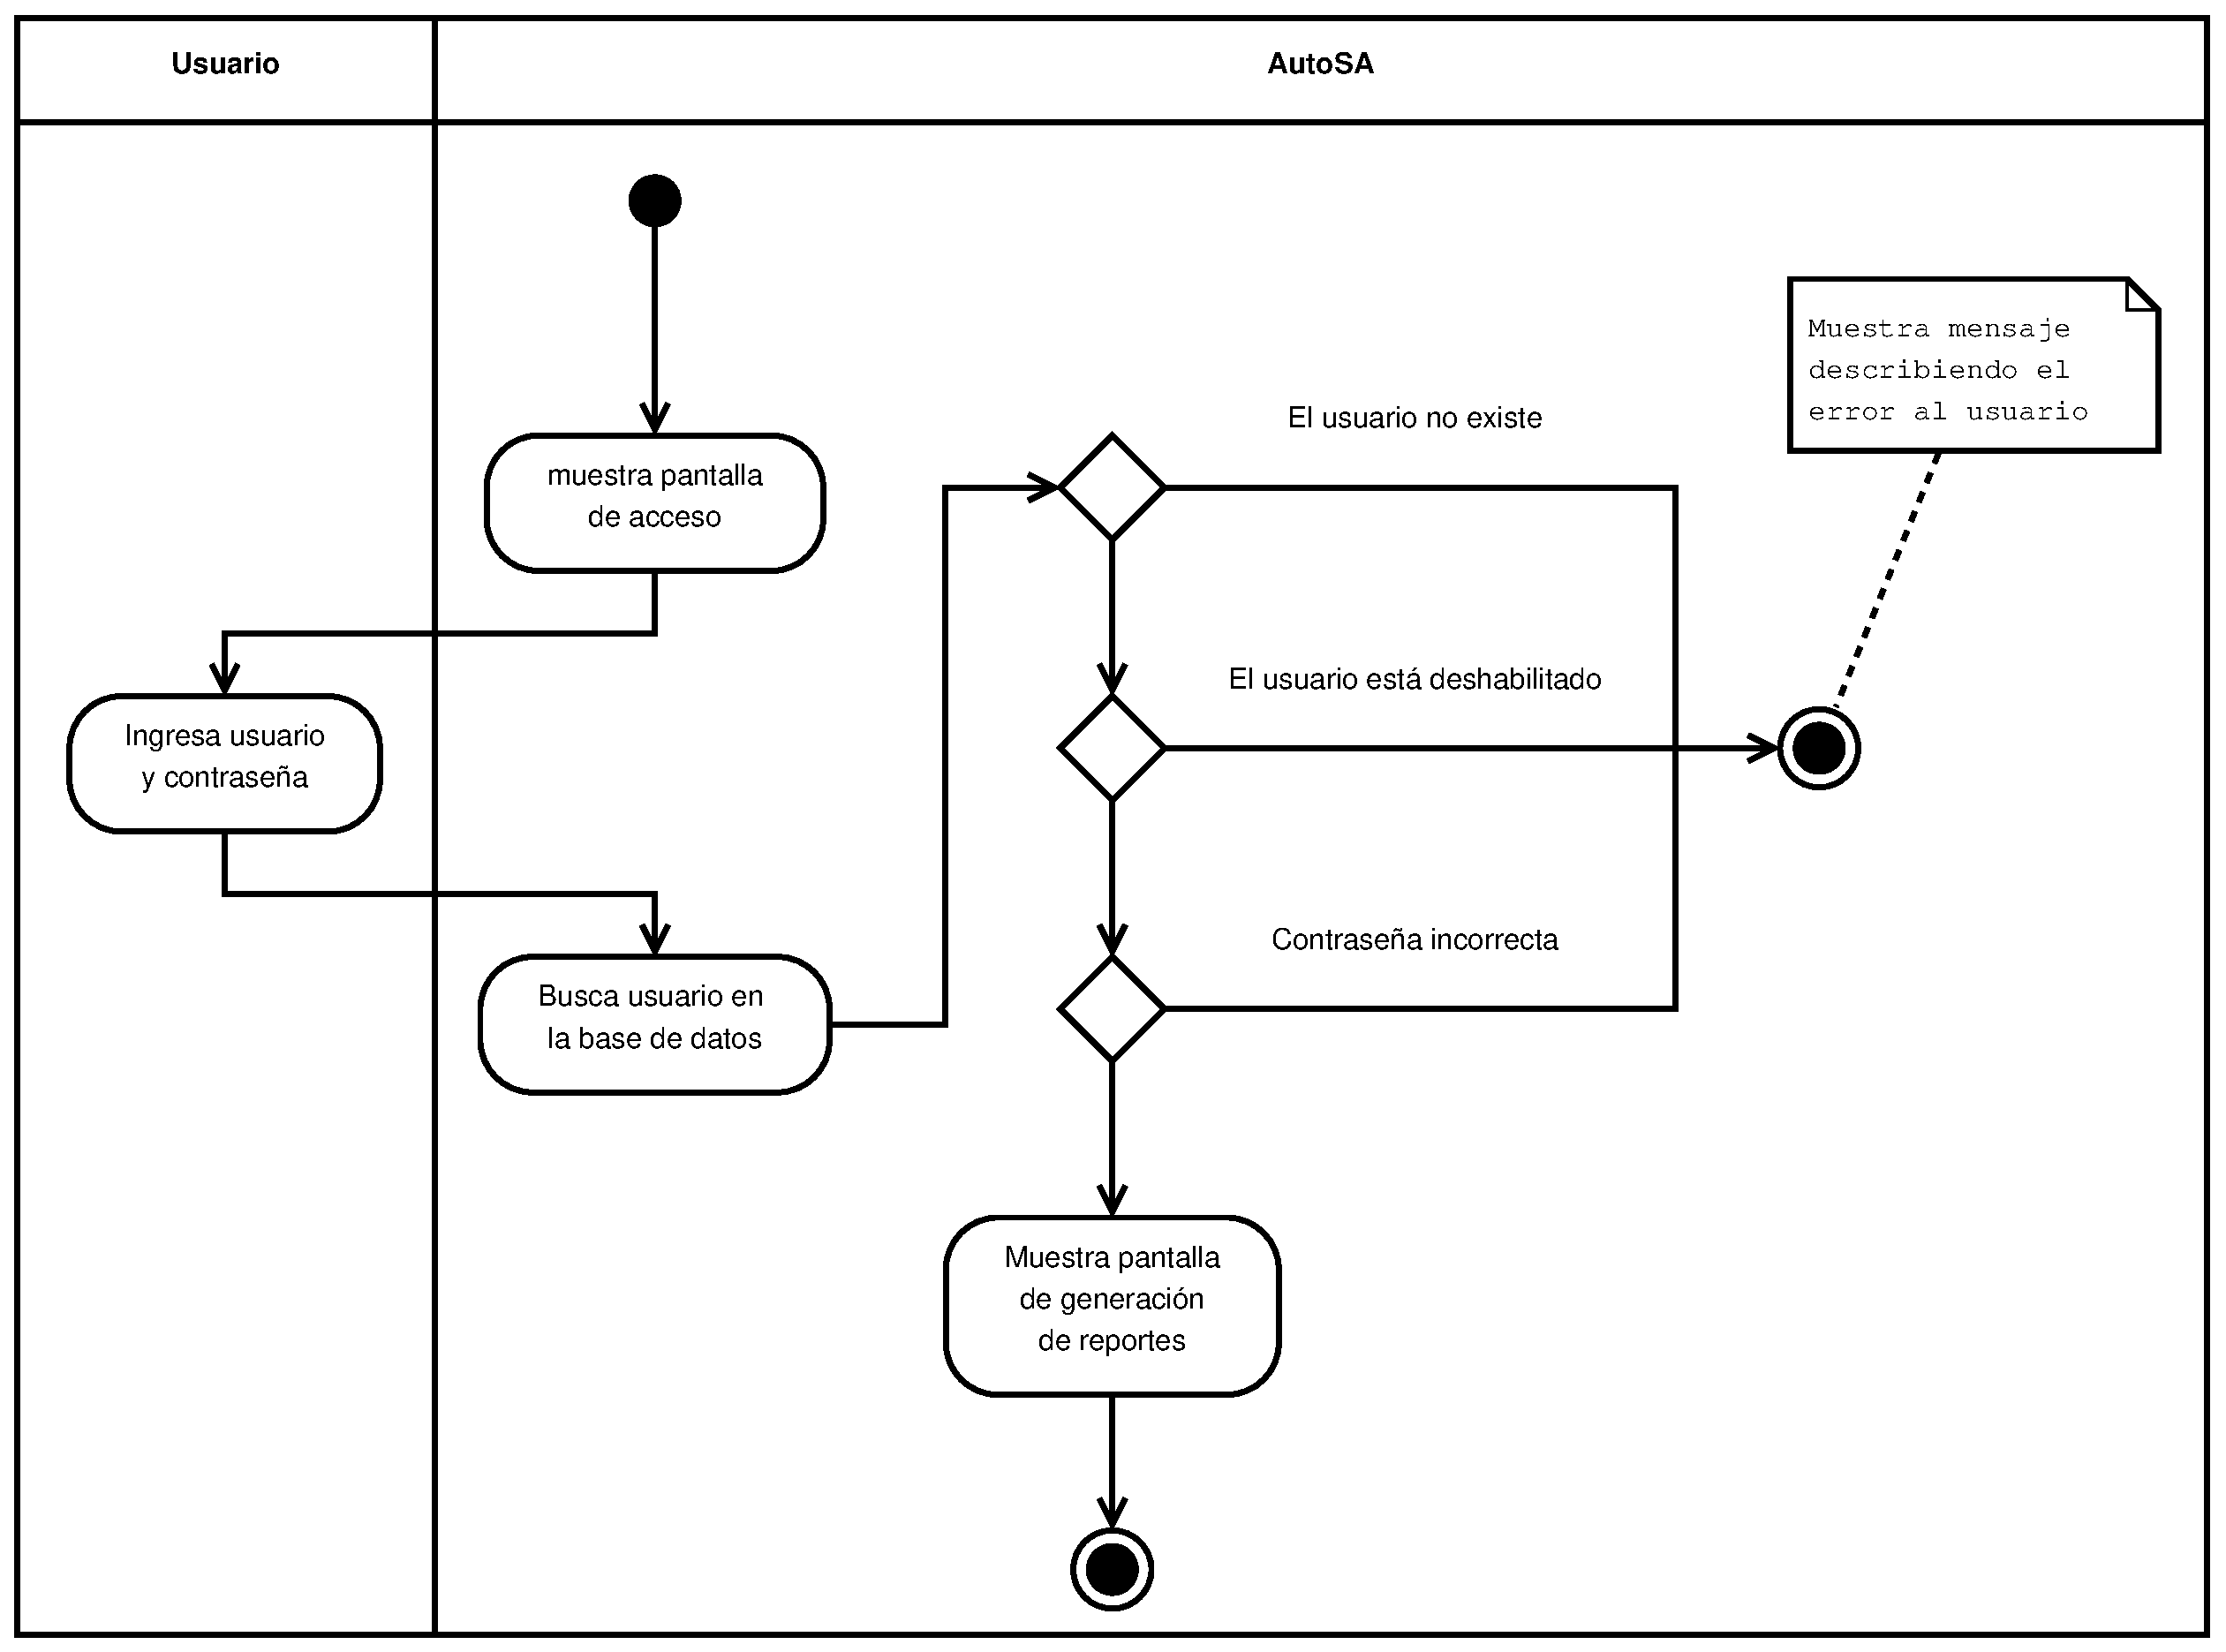
\includegraphics[width=\textwidth]{dia-activity-login}
  \caption{Diagrama de actividad del flujo de acceso al sistema.}
  \label{fig:dia-activity-login}
\end{figure}
\paragraph{Precondiciones:}
\begin{enumerate}
  \item El usuario solicita la página de acceso al sistema web.
\end{enumerate}
\paragraph{Secuencia normal:}
\begin{enumerate}
  \item El sistema muestra la pantalla de acceso.
  \item El usuario ingresa los campos:
  \begin{enumerate}
    \item Nombre de usuario.
    \item Contraseña.
  \end{enumerate}
  \item El sistema busca el nombre de usuario en la base de datos
  \item El sistema compara la contraseña provista por el usuario con el valor almacenado en la base de datos.
  \item Muestra la pantalla de generación de reportes.
\end{enumerate}
\paragraph{Postcondiciones:}
\begin{enumerate}
  \item El usuario cuenta con un código temporal de acceso a la interfaz web.
  \item Se muestra la pantalla de generación de reportes.
\end{enumerate}
\paragraph{Excepciones:}
\begin{enumerate}
  \item Los siguientes escenarios se consideran un error de autencación.
  \begin{itemize}
    \item El usuario no existe en la base de datos.
    \item El usuario tiene estado \textbf{deshabilitado}.
    \item La contraseña proporcionada no coincide con la almacenada. 
  \end{itemize}
\end{enumerate}

\subsection{Generar reporte}\label{cu-generar-reporte}
\paragraph{Identificador:}
CU-GENERAR-REPORTE
\paragraph{Actores:}
Usuario
\paragraph{Descripción:}
Este caso de uso ofrece al usuario la generación de reportes, es decir, ejecutar una consulta a la base de datos y vaciar el resultado en un archivo, como se muestra en el diagrama de actividad de la Figura \ref{fig:dia-activity-reporter}. La consulta puede ser ejecutada sobre una o más tablas, es importante mencionar que existen catálogos con claves de productos y clientes que cambian constantemente, ver caso de uso \textbf{CU-ACTUALIZAR-CATALOGO}.
\begin{figure}[h]
  \centering
  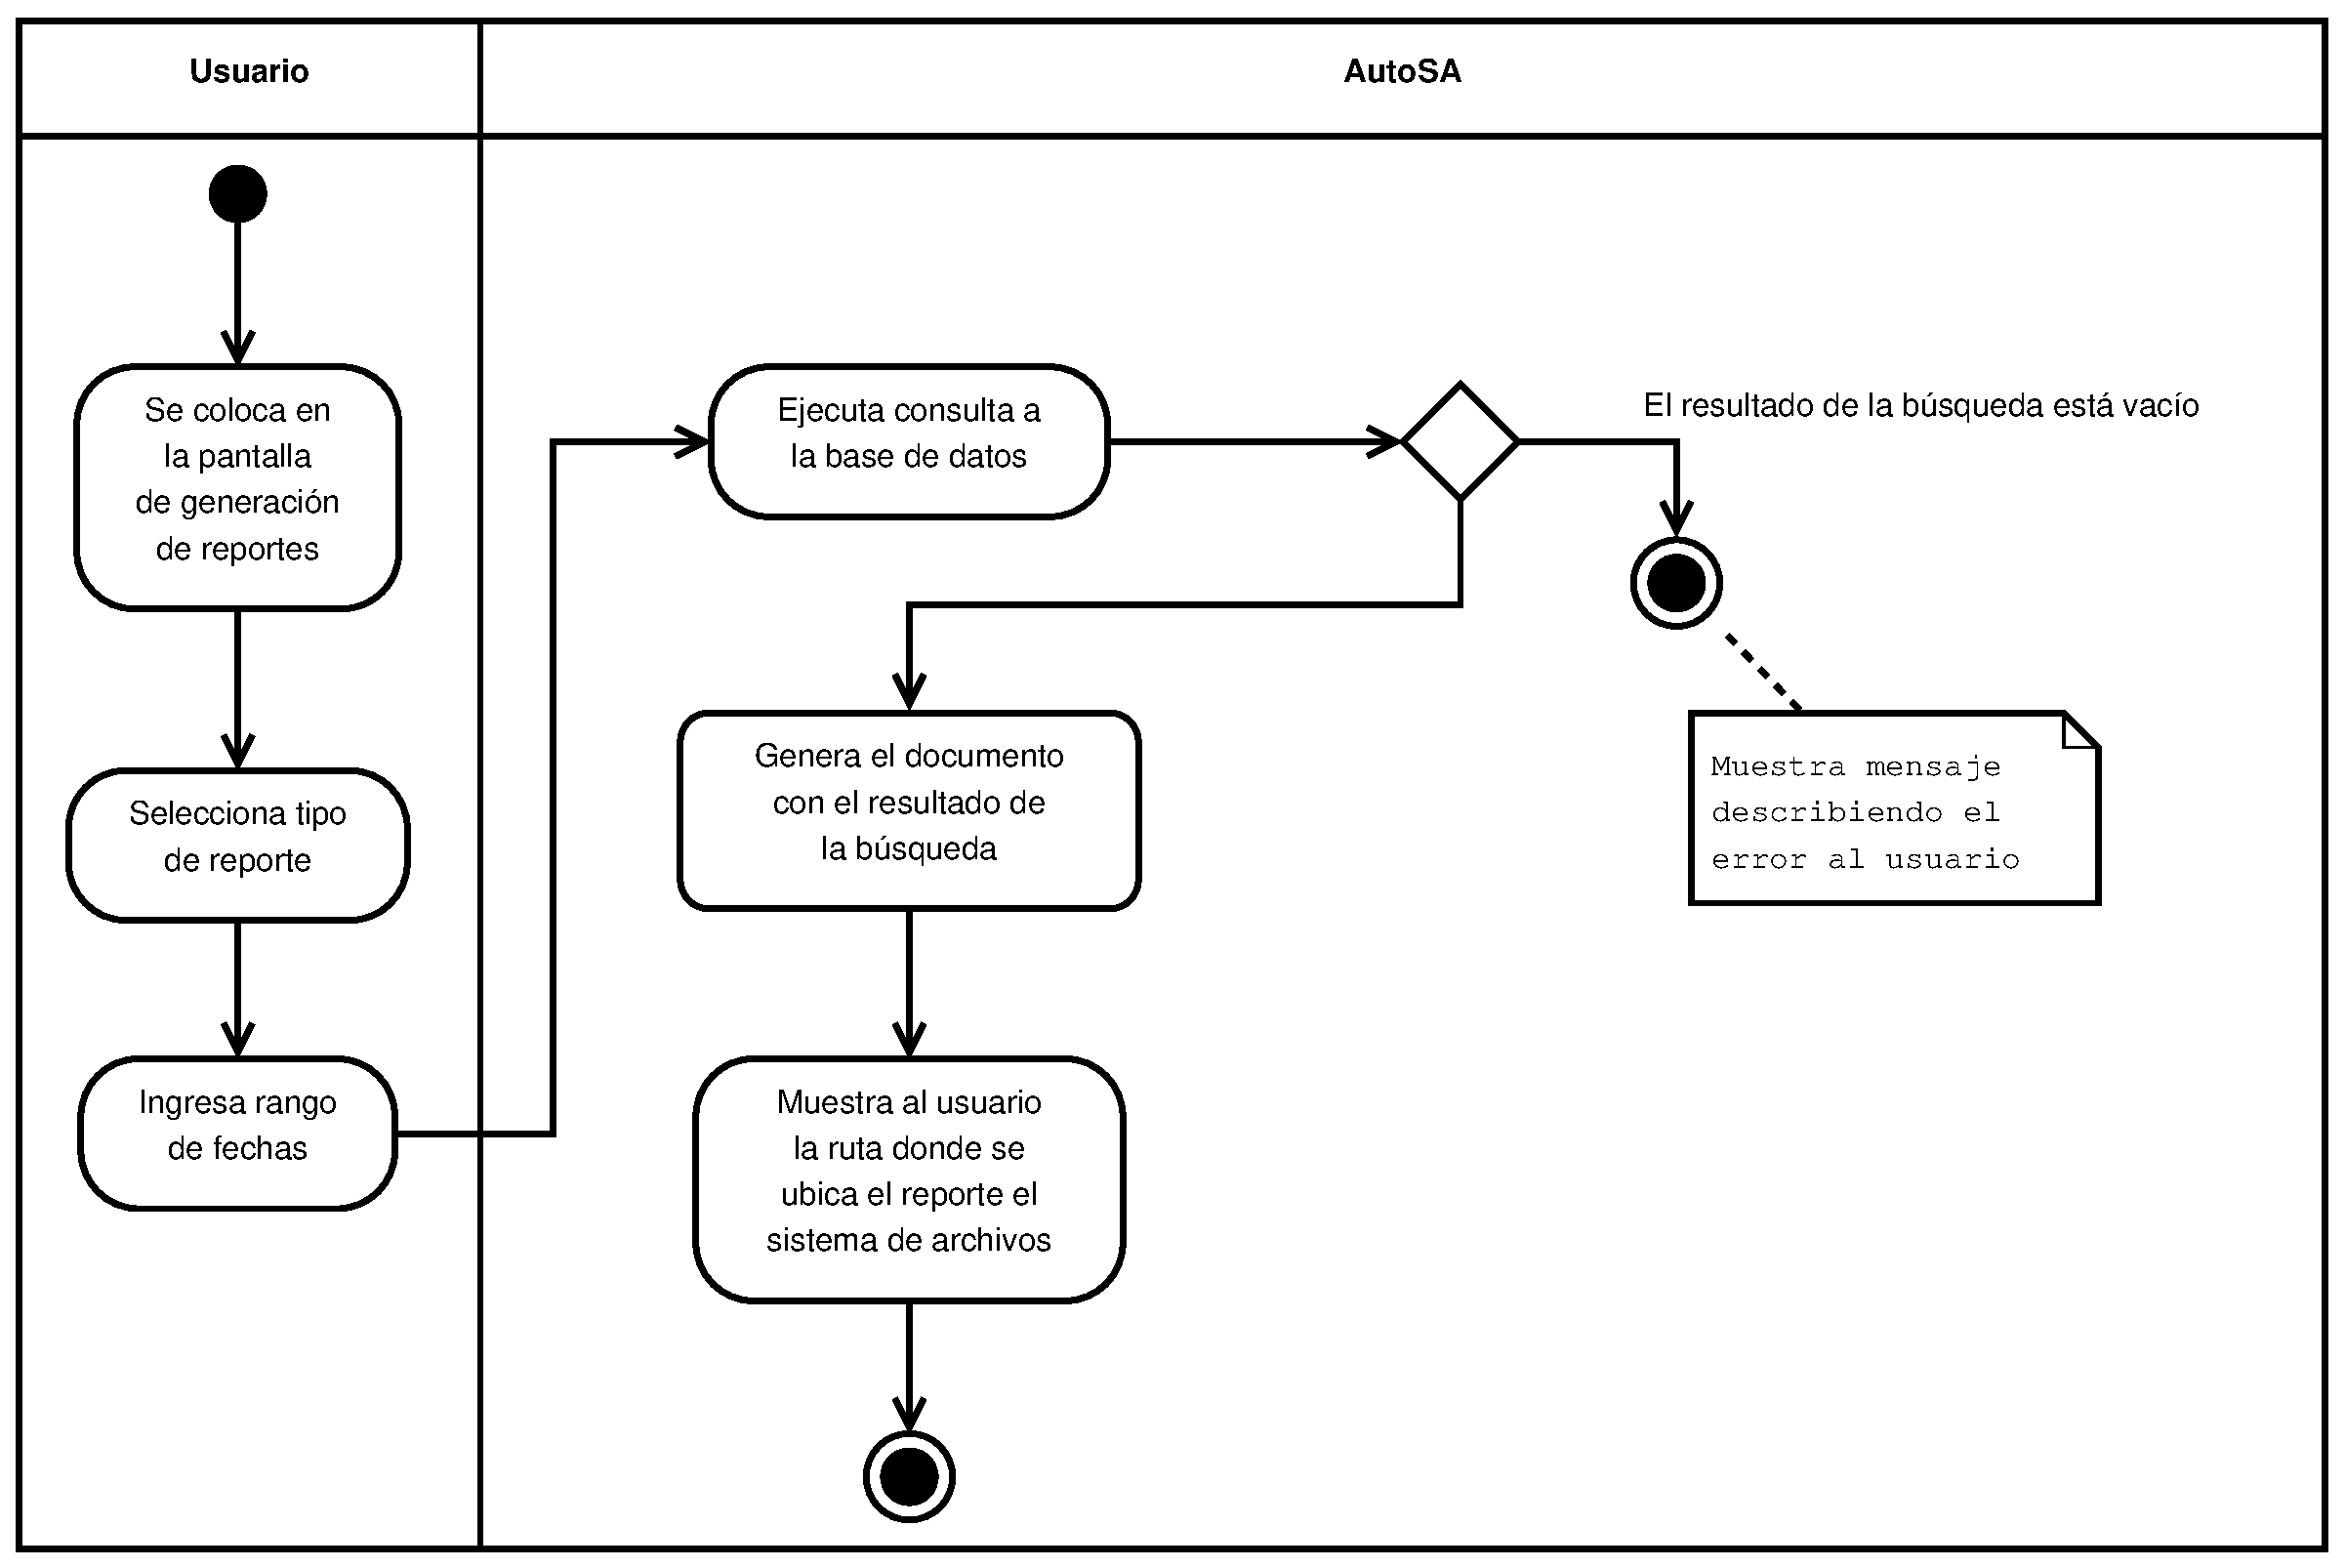
\includegraphics[width=\textwidth]{dia-activity-reporter}
  \caption{Diagrama de actividad del flujo para generación de reportes.}
  \label{fig:dia-activity-reporter}
\end{figure}
\paragraph{Precondiciones:}
\begin{enumerate}
  \item El usuario ha iniciado sesión correctamente en la interfaz web (ver caso de uso \textbf{CU-ENTRAR-WEB}).
\end{enumerate}
\paragraph{Secuencia normal:}
\begin{enumerate}
  \item El usuario navega a la pantalla de generación de reportes.
  \item En la pantalla de generación de reportes el usuario realiza las siguientes acciones:
    \begin{enumerate}
    \item Llenar el formulario de la pantalla con los siguientes campos:
    \begin{enumerate}
      \item Tipo de reporte.
      \item Fecha y hora inicial.
      \item Fecha y hora final.
    \end{enumerate}
    \item Enviar el formulario.
  \end{enumerate}
  \item El sistema ejecuta los siguientes pasos:
  \begin{enumerate}
    \item Realiza la consulta a la base de datos definida para el reporte requerido en 1.a.
    \item El resultado del paso anterior es escrito en un archivo extendido de Excel\textsuperscript{\textcopyright} y depositado en el sistema de archivos.
    \item Muestra al usuario la ruta en el sistema de archivos donde fue depositado el reporte.
  \end{enumerate}
\end{enumerate}
\paragraph{Postcondiciones:}
\begin{enumerate}
  \item El reporte se encuentra en el sistema de archivos dentro un archivo con formato extendido de Excel\textsuperscript{\textcopyright}.
\end{enumerate}
\paragraph{Excepciones:}
\begin{enumerate}
  \item Si el reporte no cuenta con registros el archivo no se genera y se muestra un mensaje al usuario indicando la situación.
\end{enumerate}


\subsection{Actualizar catálogo}\label{cu-actualizar-catalogo}
\paragraph{Identificador:}
CU-ACTUALIZAR-CATALOGO
\paragraph{Actores:}
Usuario
\paragraph{Descripción:}
Define la actualización masiva de los catálogos en la base de datos mediante un archivo ingresado por un usuario de la interfaz Web, la Figura \ref{fig:dia-activity-cat-update} muestra el diagrama de actividad para este caso de uso.
\begin{figure}[h]
  \centering
  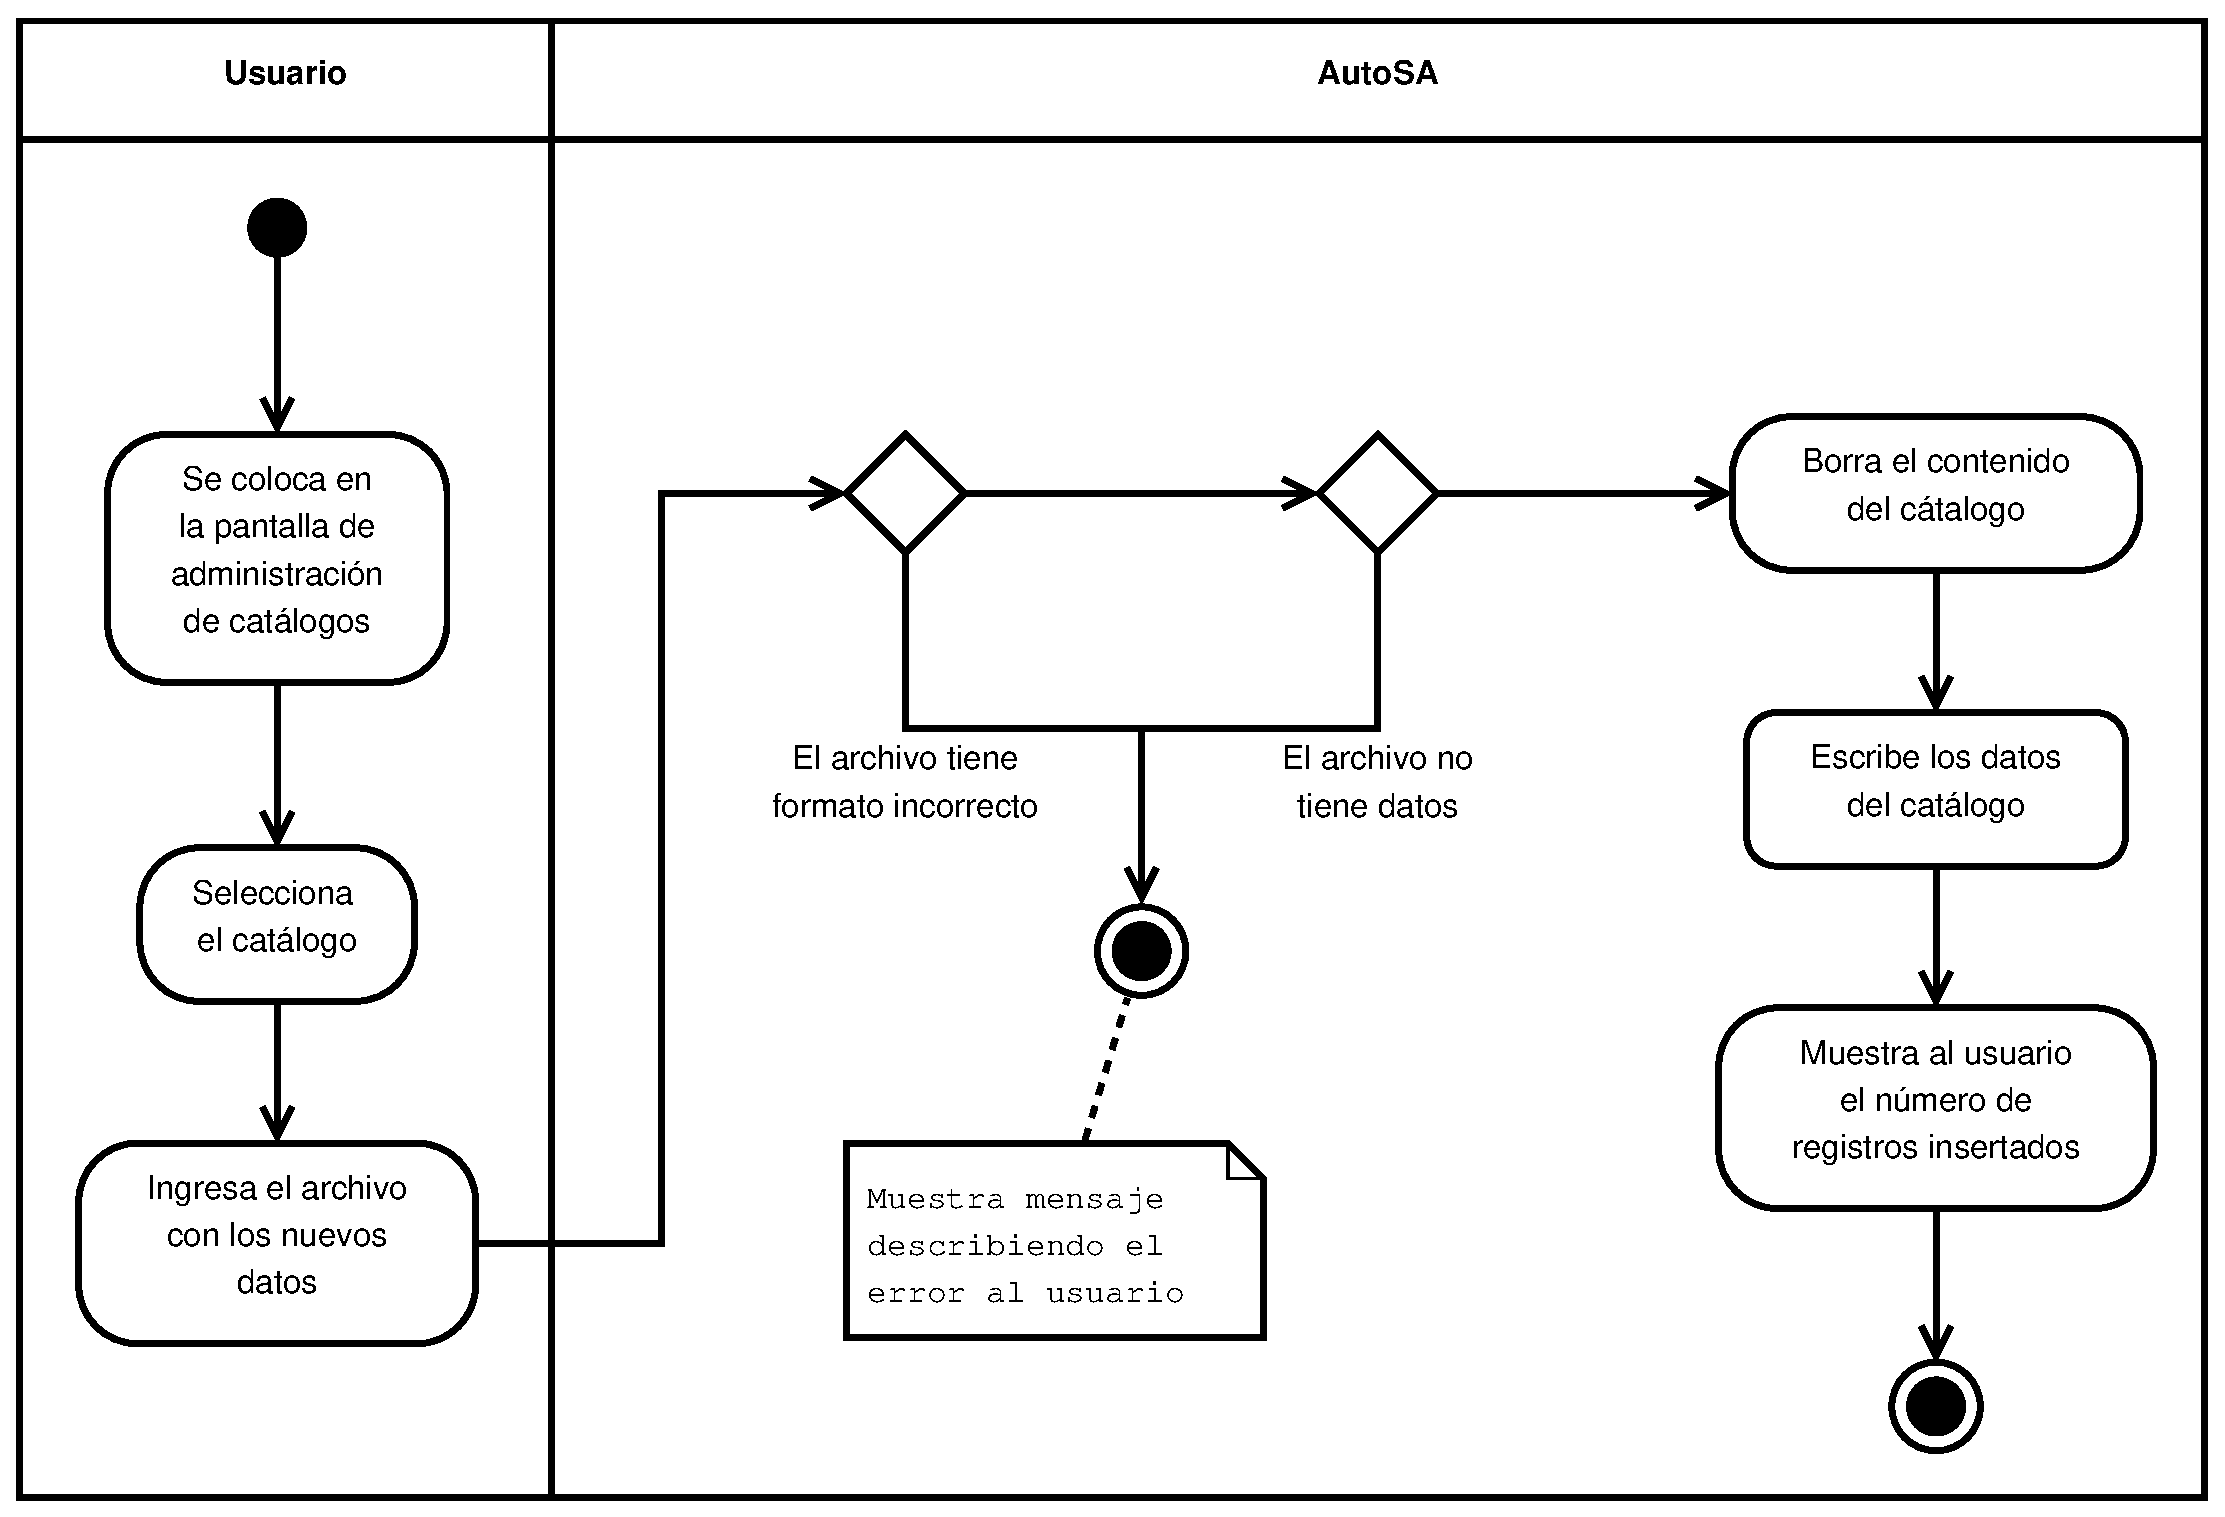
\includegraphics[width=\textwidth]{dia-activity-cat-update}
  \caption{Diagrama de actividad del flujo para la actualización de catálogos.}
  \label{fig:dia-activity-cat-update}
\end{figure}
\paragraph{Precondiciones:}
\begin{enumerate}
  \item El usuario ha iniciado sesión correctamente en la interfaz web (ver caso de uso \textbf{CU-ENTRAR-WEB}).
  \item El archivo ingresado tiene formato extendido de Excel\textsuperscript{\textcopyright}.
  \item Los catálogos que pueden ser modificados por este caso de uso son aquellos que contienen códigos de medicamentos y lugares de entrega.
\end{enumerate}
\paragraph{Secuencia normal:}
\begin{enumerate}
  \item El usuario navega a la pantalla de administración de catálogos.
  \item El usuario realiza las siguientes acciones en la pantalla de administración de catálogos:
  \begin{enumerate}
    \item Seleccionar el nombre del catálogo.
    \item Seleccionar el archivo en formato de Excel\textsuperscript{\textcopyright} que contiene la información para el catálogo.
    \item Enviar el formulario.
  \end{enumerate}
  \item El sistema sigue los siguientes pasos:
  \begin{enumerate}
    \item Valida el formato del archivo recibido.
    \item Valida que el archivo recibido contenga al menos un renglón sin contar el encabezado.
    \item Borra el contenido del catálogo en la base datos y copia la información del archivo recibido.
    \item Muestra al usuario el número de registros guardados en el catálogo después de la actualización.
  \end{enumerate}
\end{enumerate}
\paragraph{Postcondiciones:}
\begin{enumerate}
  \item El catálogo ha sido actualizado al contenido del archivo proporcionado por el usuario.
\end{enumerate}
\paragraph{Excepciones:}
\begin{enumerate}
  \item Si el archivo no cuenta con el formato solicitado, entonces se muestra un mensaje de error al usuario y se cancela la ejecución sin modificar el catálogo en la base de datos.
  \item Si el archivo no contiene ningún registro para el catálogo, entonces se muestra un mensaje de error al usuario y se cancela la ejecución sin modificar el catálogo en la base de datos.
\end{enumerate}


\subsection{Buscar órdenes}\label{cu-buscar}
\paragraph{Identificador:}
CU-BUSCAR
\paragraph{Actores:}
Usuario
\paragraph{Descripción:}
Define el flujo para la búsqueda de órdenes de reposición, la Figura \ref{fig:dia-activity-search} muestra el diagrama de actividad para este caso de uso.
\begin{figure}[h]
  \centering
  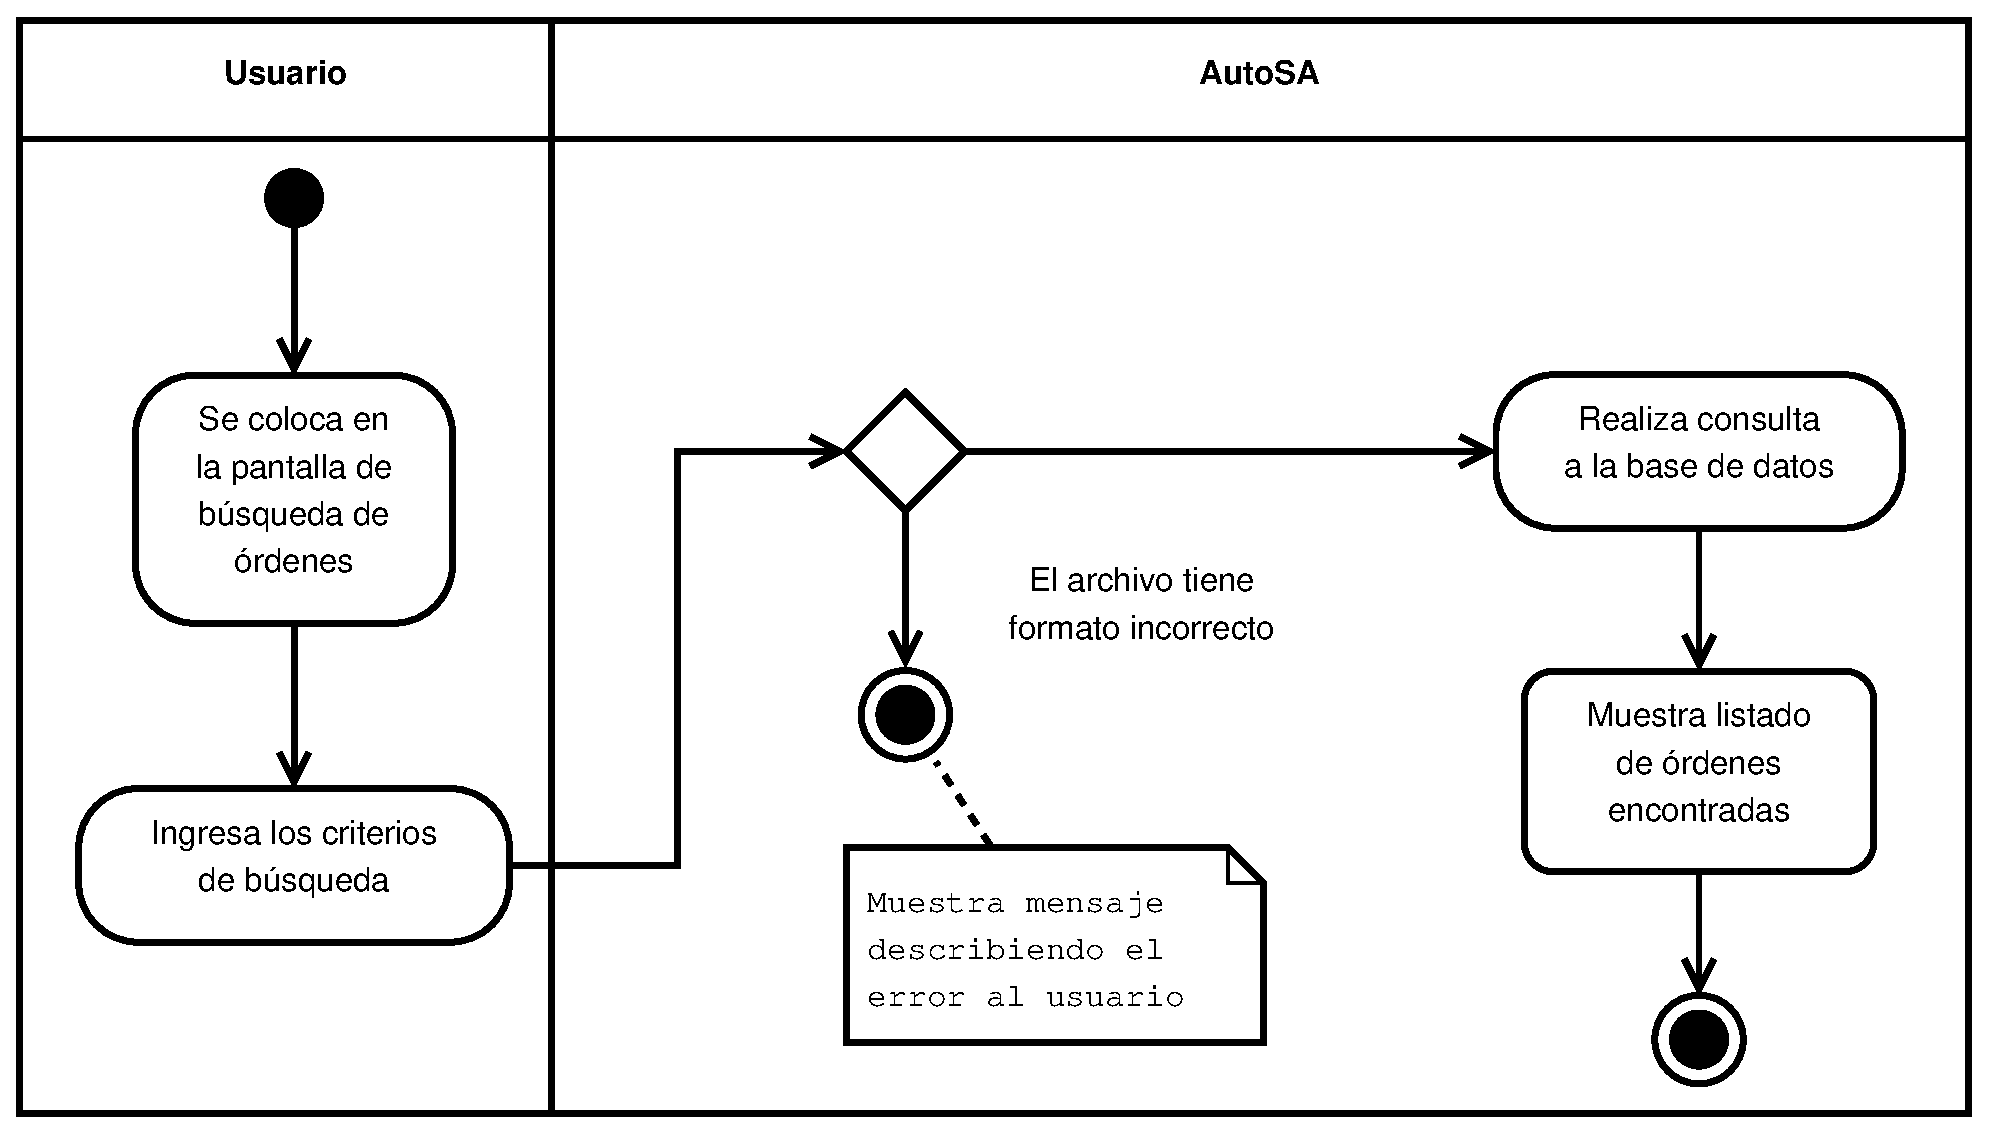
\includegraphics[width=\textwidth]{dia-activity-search}
  \caption{Diagrama de actividad del flujo para la búsqueda de órdenes de reposición.}
  \label{fig:dia-activity-search}
\end{figure}
\paragraph{Precondiciones:}
\begin{enumerate}
  \item El usuario ha iniciado sesión correctamente en la interfaz web (ver caso de uso \textbf{CU-ENTRAR-WEB}).
\end{enumerate}
\paragraph{Secuencia normal:}
\begin{enumerate}
  \item El usuario navega a la pantalla de búsqueda de órdenes de reposición.
  \item El usuario realiza ingresa los criterios para la búsqueda presentados en el filtro:
  \begin{enumerate}
    \item Número de orden.
    \item Estatus de atención.
    \item Rango de fechas en que fueron atendidas las órdenes de reposición.
  \end{enumerate}
  \item El sistema muestra el resultado de la búsqueda. Para cada orden de reposición listada se muestra un enlace que lleva a la visualización de la orden (ver casos de uso \textbf{CU-VISUALIZAR}).
\end{enumerate}
\paragraph{Postcondiciones:}
\begin{enumerate}
  \item Se muestra un listado con las órdenes de reposición que cumplen con el filtro definido por el usuario durante el caso de uso.
\end{enumerate}
\paragraph{Excepciones:}
\begin{enumerate}
  \item En caso de no contar con una conexión a la base de datos se muestra un mensaje de error informando al usuario.
\end{enumerate}


\subsection{Visualizar orden}\label{cu-visualizar}
\paragraph{Identificador:}
CU-VISUALIZAR
\paragraph{Actores:}
Usuario
\paragraph{Descripción:}
La forma en que el usuario de la interfaz web es capaz de visualizar los datos de una orden de reposición, en la Figura \ref{fig:dia-activity-view} se muestra el diagrama de actividad que sigue este caso de uso, para llegar a esta sección es necesario que el usuario haya ejecutado la búsqueda de órdenes de reposición y seleccionado la orden para visualizar como se muestra en la Figura \ref{fig:dia-casos-uso} (ver caso de uso \textbf{CU-BUSCAR}).
\begin{figure}[h]
  \centering
  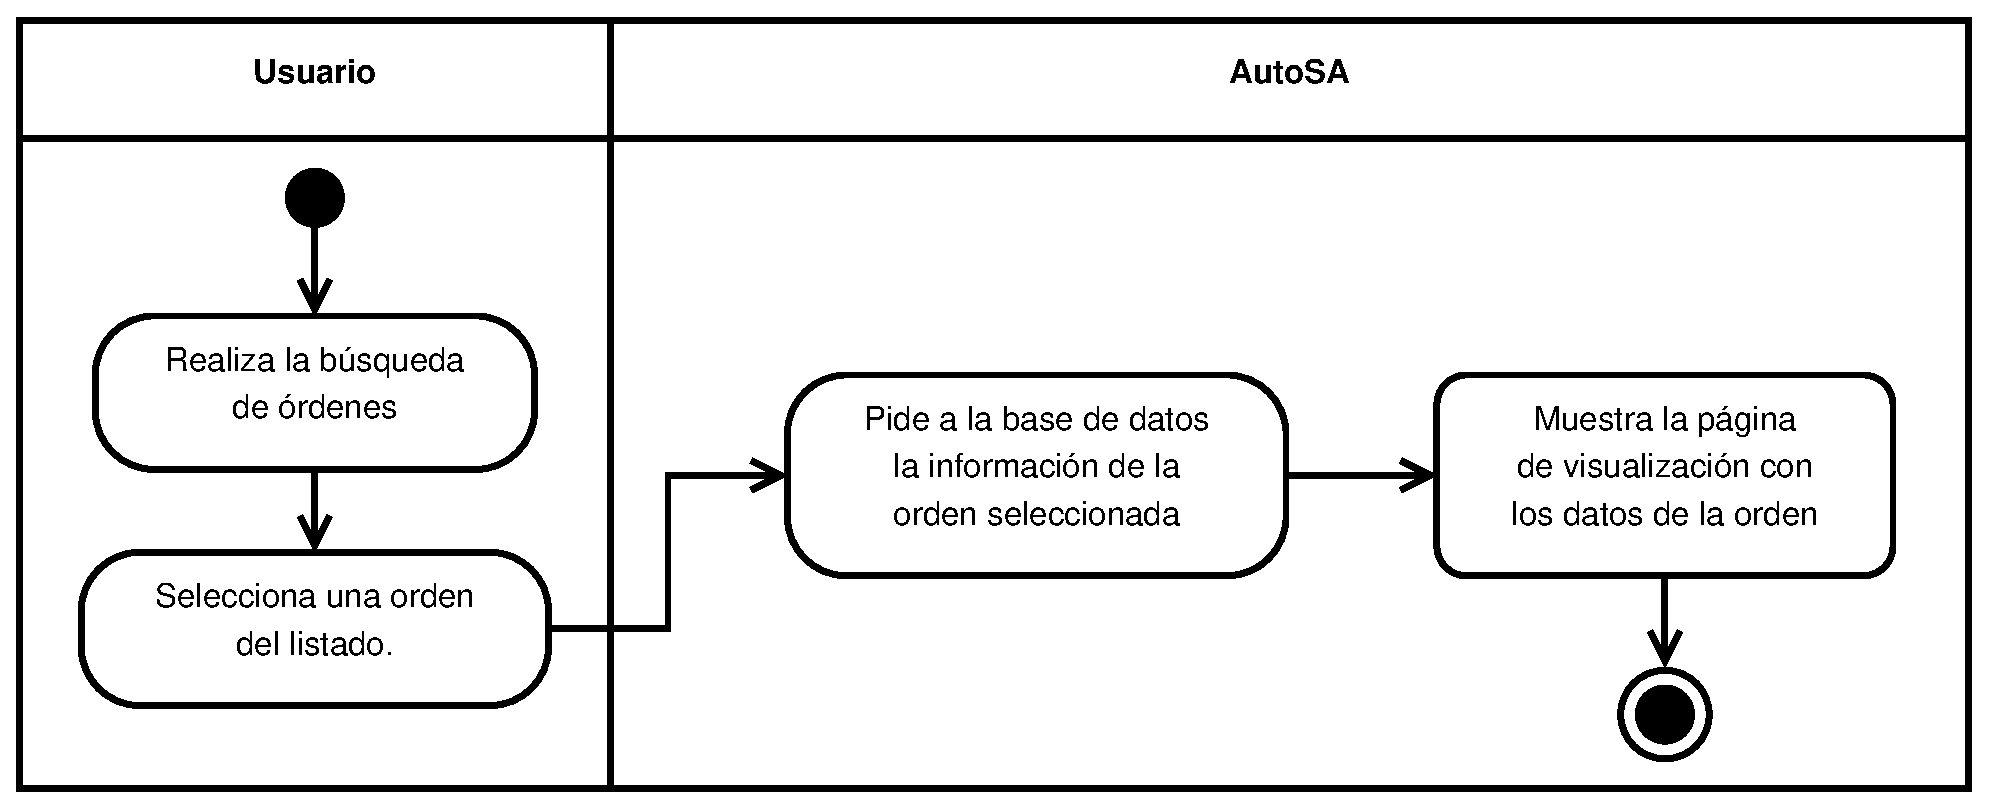
\includegraphics[width=\textwidth]{dia-activity-view}
  \caption{Diagrama de actividad del flujo para la visualización de los datos de una orden de reposición.}
  \label{fig:dia-activity-view}
\end{figure}
\paragraph{Precondiciones:}
\begin{enumerate}
  \item El usuario ha iniciado sesión correctamente en la interfaz web (ver caso de uso \textbf{CU-ENTRAR-WEB}).
  \item El usuario localiza la orden de reposición que desea visualizar (ver caso de uso \textbf{CU-BUSCAR})
\end{enumerate}
\paragraph{Secuencia normal:}
\begin{enumerate}
  \item El usuario navega a la pantalla de visualización de la orden de reposición seleccionada (ver caso de uso \textbf{CU-BUSCAR}).
  \item Se muestra la pantalla con los datos de la orden:
  \begin{enumerate}
    \item Se muestran todos los datos capturados del Sistema de Abastecimiento durante el procedimiento de atención.
    \item También se muestran los estados de atención, es decir, el estado en el Sistema de Abastecimiento  y el estado de atención.
  \end{enumerate}
  \item Se muestran enlaces para que el usuario pueda editar los datos de la orden (ver caso de uso \textbf{CU-EDITAR}) y también para generar el acuse de envío (ver caso de uso \textbf{CU-GENERAR-ACUSE}).
  \item En caso de seleccionar la generación del acuse de envío se ejecuta el caso de uso \textbf{CU-GENERAR-ACUSE}.
\end{enumerate}
\paragraph{Postcondiciones:}
\begin{enumerate}
  \item Se muestra una pantalla al usuario con los datos de la orden de reposición solicitada, además las opciones para editar y generar el acuse de envío.
\end{enumerate}
\paragraph{Excepciones:}
\begin{enumerate}
  \item En caso de no contar con una conexión a la base de datos se muestra un mensaje de error informando al usuario.
\end{enumerate}


\subsection{Editar orden}\label{cu-editar}
\paragraph{Identificador:}
CU-EDITAR
\paragraph{Actores:}
Usuario
\paragraph{Descripción:}
La forma en que el usuario de la interfaz web puede modificar los datos de una orden de reposición que está visualizando, en la Figura \ref{fig:dia-activity-edit} se muestra el diagrama de actividad que sigue este caso de uso, para llegar a esta vista es necesario que el usuario haya ejecutado la visualización de la orden de reposición que desea modificar. La dependencia de este caso de uso se muestra en la Figura \ref{fig:dia-casos-uso} (ver caso de uso \textbf{CU-BUSCAR}).
\begin{figure}[h]
  \centering
  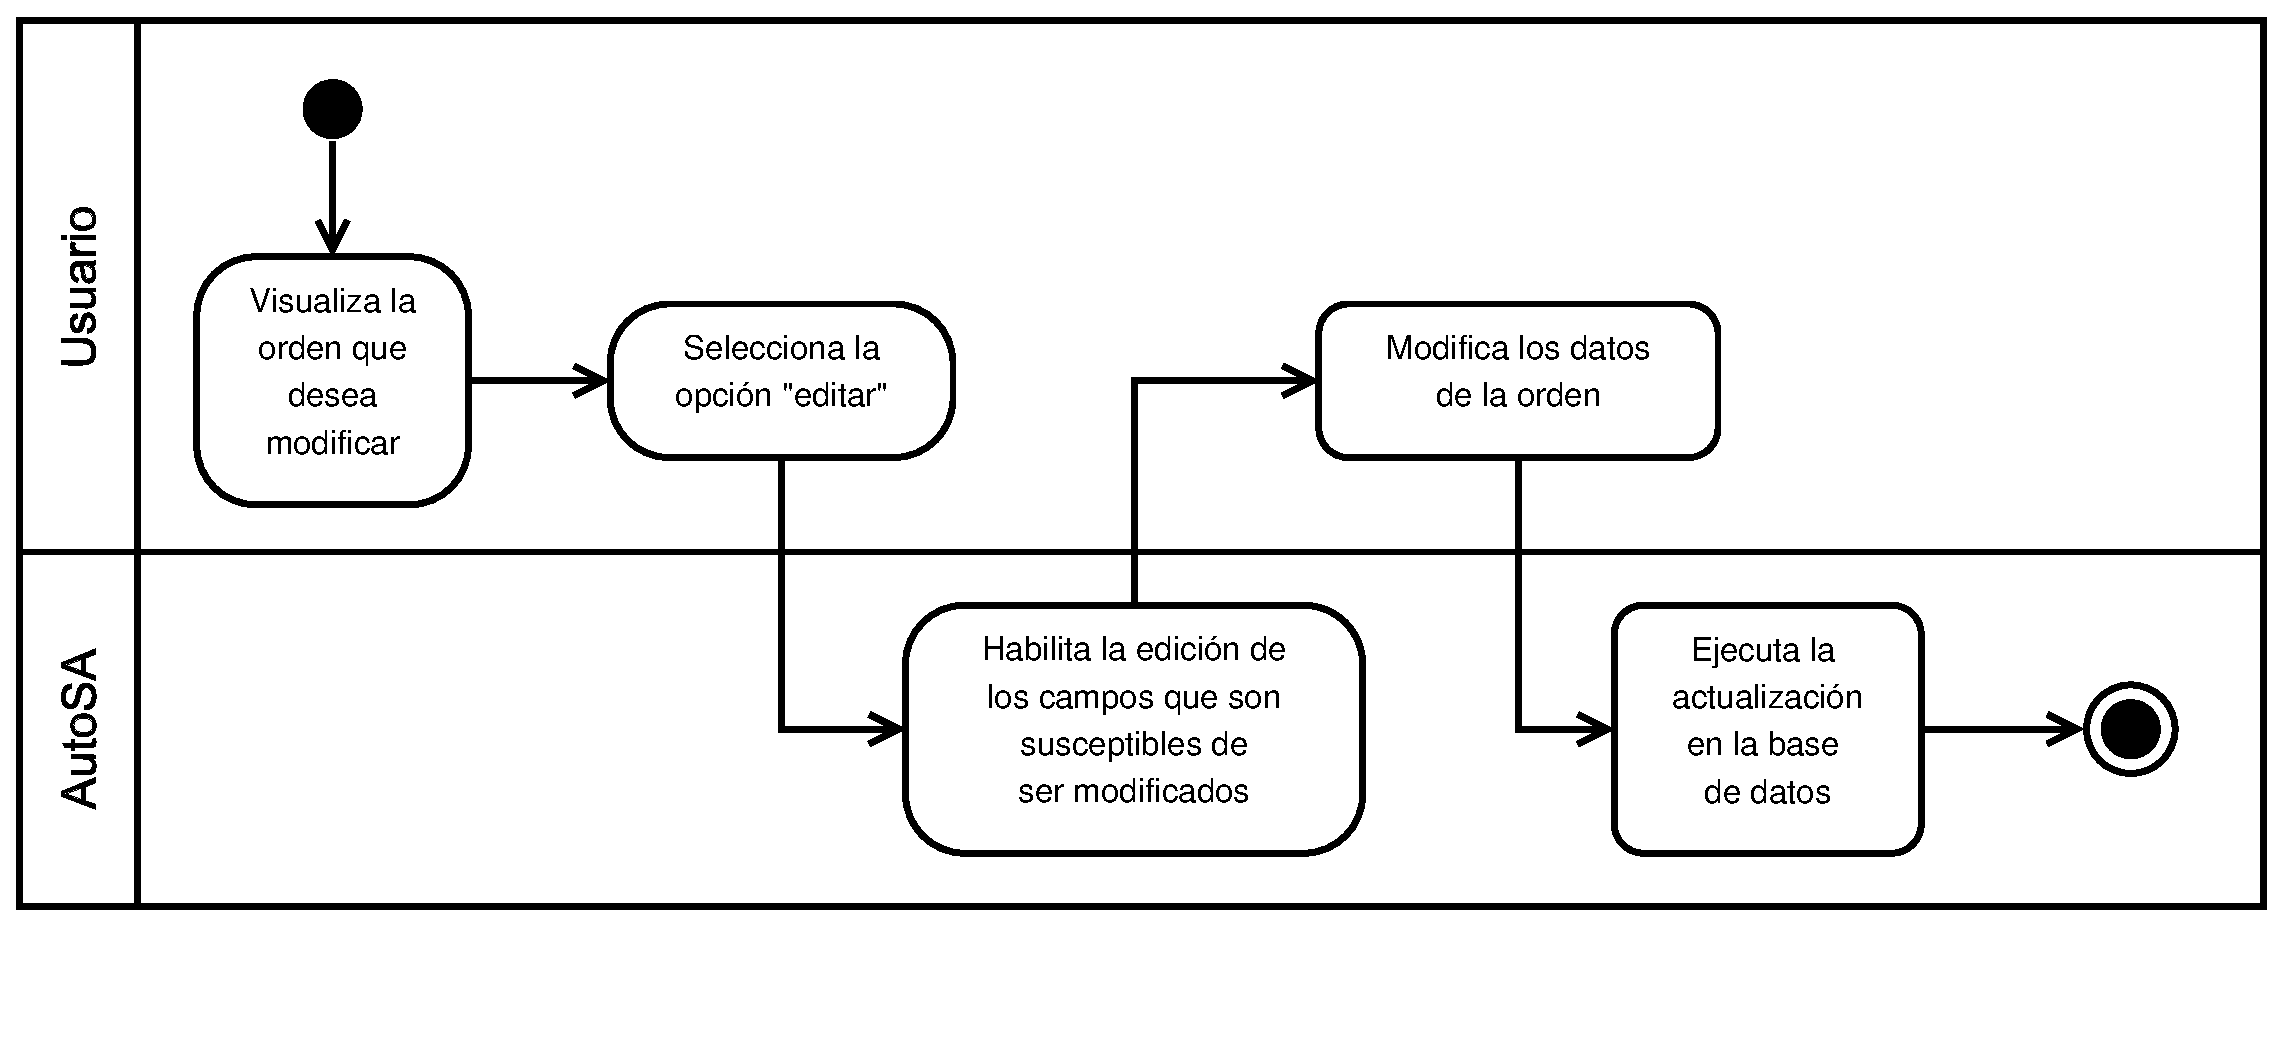
\includegraphics[width=\textwidth]{dia-activity-edit}
  \caption{Diagrama de actividad del flujo para la modificar de los datos de una orden de reposición.}
  \label{fig:dia-activity-edit}
\end{figure}
\paragraph{Precondiciones:}
\begin{enumerate}
  \item El usuario ha iniciado sesión correctamente en la interfaz web (ver caso de uso \textbf{CU-ENTRAR-WEB}).
  \item El usuario visualiza la orden de reposición que desea editar (ver caso de uso \textbf{CU-VISUALIZAR}).
  \item Los campos utilizados para identificar unívocamente la orden de reposición no podrán ser modificados. 
\end{enumerate}
\paragraph{Secuencia normal:}
\begin{enumerate}
  \item El usuario navega a la pantalla de edición con la orden de reposición visualizada (ver caso de uso \textbf{CU-VISUALIZAR}).
  \item Modificar cualquiera de los campos modificables.
  \item Seleccionar el botón Guardar.
\end{enumerate}
\paragraph{Postcondiciones:}
\begin{enumerate}
  \item Los datos modificados por el usuario en la interfaz web se encuentran almacenados en la base de datos.
\end{enumerate}
\paragraph{Excepciones:}
\begin{enumerate}
  \item En caso de no contar con una conexión a la base de datos se muestra un mensaje de error informando al usuario.
\end{enumerate}

\section{Resumen}
Se han definido el el alcance del proyecto que comprende la automatización de los procesos realizados por los operadores del Sistema de Abastecimiento hasta la generación del formato de salida, el alcance de la interfaz web comprende las tareas de modificación de órdenes de reposición atendidas, generación de reportes y actualización de catálogos.\\
Bajo los puntos anteriores se han definido los casos de uso que reflejan el comportamiento esperado del sistema para la automatización de procesos y la interfaz web.

\chapter{Diseño del proyecto}\label{cap3}
Conforme a lo visto en el Capítulo \ref{cap2}, el proyecto AutoSA requiere ser ejecutado de dos formas distintas:
\begin{enumerate}
 	\item Rutinas automatizadas: se ejecutan a partir del entorno gráfico del sistema operativo.
 	\item Portal de usuario: se ofrece como una página web, la cual depende del servidor web de la farmacéutica y del explorador web del usuario.
\end{enumerate}
Por otro lado es necesario contar con una base de datos la cual debe mantener los datos de las órdenes de reposición persistentes, también es necesario mantener el acceso al sistema de archivos para guardar las capturas de pantalla de las órdenes de reposición enviadas.\\
Por lo que es necesario tener dos ambientes de ejecución, la automatización que será ejecutada exclusivamente en el sistema operativo y la de web, que se ejecuta en el sistema operativo y en el explorador de Internet del usuario.


%===============================================================================
%===============================================================================


\section{Diseño de la arquitectura del sistema AutoSA}
Bourque define la arquitectura de software como:
\begin{quote}
	El conjunto de estructuras necesarias para la comprensión de un sistema en el cual se comprometen elementos de software, relaciones entre ellos y sus propiedades\cite{SWEBOOK}.
\end{quote}
En las últimas décadas la arquitectura de software ha profundizado en el estudio genérico de las estructuras del software, dando lugar a técnicas como los patrones de diseño (ver Apéndice \ref{sec-patrones}) \cite{SWEBOOK, SoftwareArchitectureInAction}.

Siguiendo el concepto de arquitectura, se muestran los componentes del sistema y su respectiva solución a los casos de uso del Capítulo \ref{sec:casos-uso}.

\subsection{Componentes del sistema AutoSA}
El diagrama de componentes sirve para visualizar los componentes en los que se divide el sistema y las interfaces por las cuales se comunican tales componentes. El la Figura \ref{fig:dia-components} se muestra el diagrama de componentes para el sistema AutoSA. En las secciones consecuentes se describe cada componente y las interfaces que ofrece\footnote{Únicamente se mostrarán los diagramas de secuencia más completos que reflejan un comportamiento no trivial.}.
\begin{figure}[h]
\centering
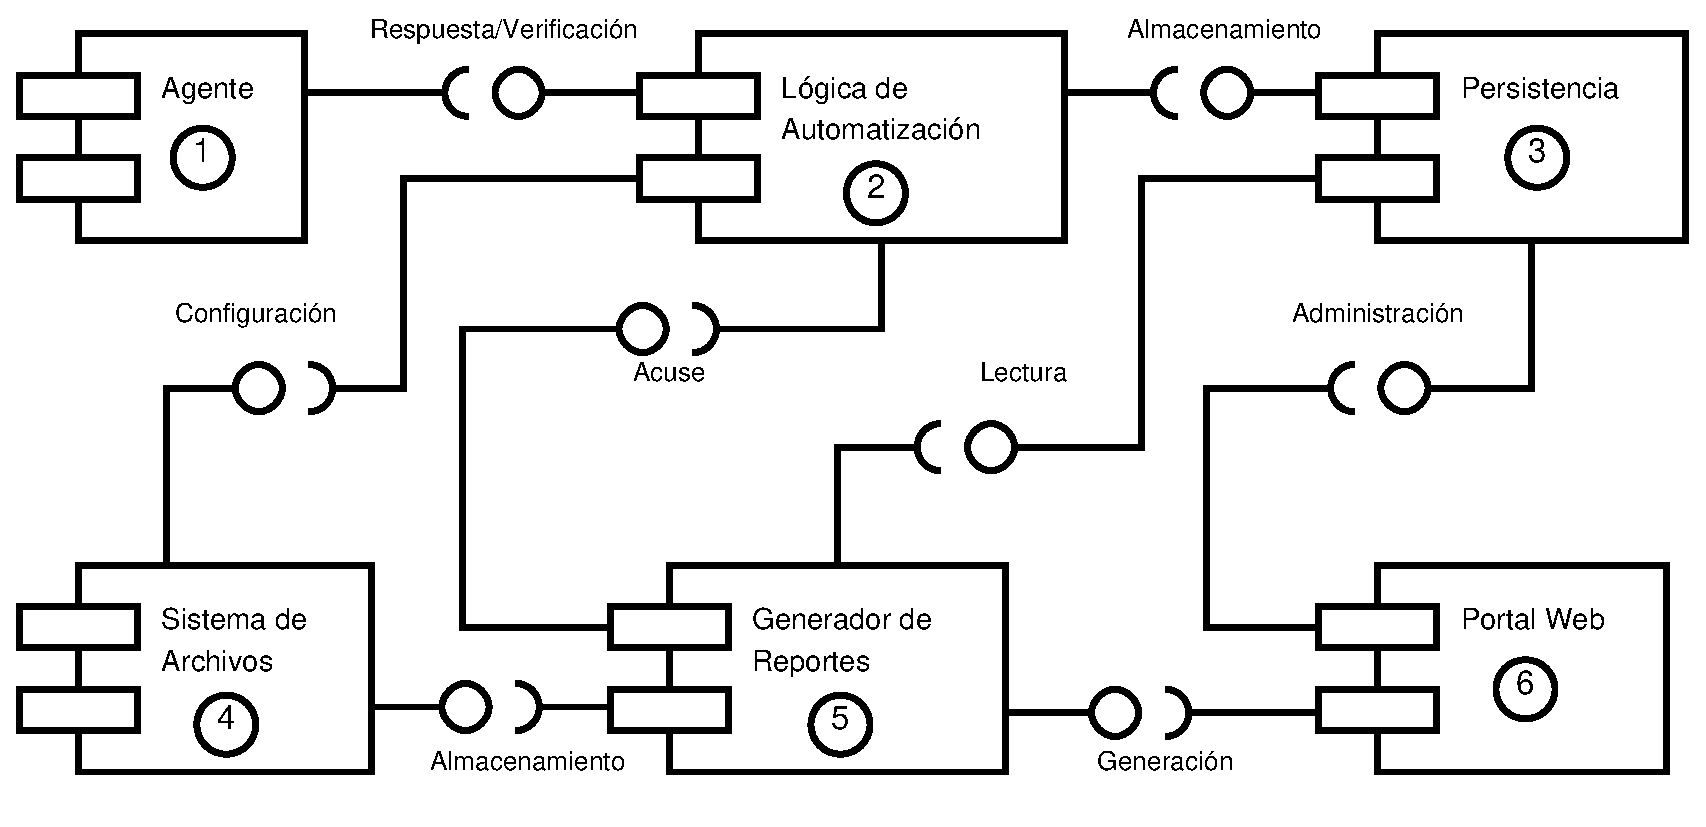
\includegraphics[width=\textwidth]{dia-components}
\caption{Diagrama de componentes.}
\label{fig:dia-components}
\end{figure}

\subsubsection{Agente}
El componente que contiene y ejecuta las rutinas de automatización, esto es mediante una interfaz con el usuario en la cual puede seleccionar el proceso a ser ejecutado. No ofrece interfaces a los demás componentes, consume exclusivamente el componente de \textbf{Lógica de Automatización}.

\subsubsection{Lógica de automatización}
La función de este componente es de ejecutar las reglas de negocio necesarias para en los flujos de los procesos de automatización, ofrece las interfaces de respuesta y verificación.
\paragraph{Interfaz Respuesta\\}
Provee el acceso a las reglas de negocio del proceso de respuesta de órdenes de reposición (ver caso de uso \ref{cu-contestar}). Esta interfaz expone las siguientes operaciones:
\begin{enumerate}
	\item \textbf{guardar-orden-nueva}: guarda un listado de nuevas órdenes de reposición.
	\item \textbf{obtener-orden-contestar}: da la siguiente orden de reposición para contestar.
	\item \textbf{obtener-datos-respuesta}: da los datos necesarios para llenar los formularios para contestar una orden de reposición en el Sistema de Abastecimiento.
	\item \textbf{actualizar-orden-contestada}: actualiza los datos almacenados de la orden de reposición con los datos de la respuesta en el  Sistema de Abastecimiento. Utiliza el componente de persistencia para actualizar los datos.
	\item \textbf{obtener-orden-enviar}: da la siguiente orden de reposición para enviar.
	\item \textbf{guardar-orden-enviada}: actualiza los datos almacenados de la orden de reposición con los datos de la pantalla de envío del Sistema de Abastecimiento. Utiliza el componente de persistencia para actualizar los datos.
	\item \textbf{obtener-acuse-envio}: solicita la generación de el acuse de envío al componente de reportes y almacena el documento el componente de Sistema de Archivos.
\end{enumerate}

\paragraph{Interfaz Verificación\\}
Provee el acceso a las reglas de negocio del proceso de verificación de órdenes de reposición canceladas. Esta interfaz expone las siguientes operaciones:
\begin{enumerate}
	\item \textbf{obtener-rango-verificar}: obtiene el rango de fechas para ingresar en el formulario de búsqueda del Sistema de Abastecimiento. El número de días que comprende el rango se obtiene utilizando el componente de Sistema de Archivos.
	\item \textbf{actualizar-estado-sa}: actualiza el EstadoSA de las órdenes de reposición recibidas a \textbf{Cancelada}. Utiliza el componente de persistencia para la actualización de datos.
\end{enumerate}

\subsubsection{Persistencia}
El componente de persistencia está basado en el patrón de diseño \textit{DAO} (ver Apéndice \ref{sec-dao}) para controlar el acceso a la base de datos\footnote{En adelante se utilizará \textbf{DAO} para hacer referencia al patrón y la instancia (objeto) del patrón.}.\\
El componente de persistencia de el proyecto AutoSA presenta las siguientes interfaces de búsqueda y almacenamiento:
\paragraph{Interfaz Almacenamiento\\}
Conjunto de operaciones diseñadas para responder a las necesidades de almacenamiento en los flujos para responder y verificar órdenes de reposición\footnote{Ver casos de uso \ref{cu-contestar}, \ref{cu-guardar-nueva}, \ref{cu-responder-orden}, \ref{cu-enviar-orden} y \ref{cu-actualizar-estatus-sa}.}. Esta interfaz expone las siguientes operaciones:
\begin{enumerate}
	\item \textbf{guardar-nueva}: inserta una nueva orden de reposición en la base de datos.
	\item \textbf{cambiar-estado}: cambia el estado de atención de una orden de reposición.
	\item \textbf{guardar-respuesta}: guarda los datos de los formularios de la pantalla de respuesta de las órdenes de reposición.
	\item \textbf{guardar-folio-acuse}: guarda el folio de acuse de envío de la orden de reposición.
	\item \textbf{actualizar-estado-sa}: actualiza el estado de atención en el Sistema de Abastecimiento a \textbf{cancelada} de las órdenes de reposición recibidas.
	\item \textbf{registrar-evento}: registra en la base de datos un evento que ocurre durante los procesos automatizados, el evento puede ser de carácter informativo o de error.
\end{enumerate}

\paragraph{Interfaz Lectura\\}
Conjunto de operaciones diseñadas para las necesidades de lectura de órdenes de reposición en los flujos para responder y verificar órdenes de reposición\footnote{Ver casos de uso \ref{cu-contestar}, \ref{cu-enviar-orden} y \ref{cu-generar-acuse}.}. Esta interfaz expone las siguientes operaciones:
\begin{enumerate}
	\item \textbf{siguiente-orden-contestar}: entrega un mapa con los datos de la primera orden de reposición encontrada con estado \textbf{Nueva}.
	\item \textbf{siguiente-orden-enviar}: entrega un mapa con los datos de la primera orden de reposición encontrada con estado \textbf{Contestada}.
	\item \textbf{obtener-datos-acuse}: obtiene los datos de una orden de reposición necesarios para generar el documento de acuse de envío.
\end{enumerate}

\paragraph{Interfaz Administración\\}
Son las operaciones que permiten modificar datos específicos de las órdenes de reposición contenidas en la base de datos, también ofrece la actualización masiva de catálogos\footnote{Ver casos de uso \ref{cu-entrar-web}, \ref{cu-generar-reporte}, \ref{cu-actualizar-catalogo}, \ref{cu-buscar}, \ref{cu-visualizar} y \ref{cu-editar}.}). Esta interfaz expone las siguientes operaciones:
\begin{enumerate}
	\item \textbf{buscar-credenciales}: busca las credenciales del usuario.
	\item \textbf{extraer-reporte}: ejecuta la búsqueda necesaria para extraer los datos del reporte indicado.
	\item \textbf{actualizar-catalogo}: actualiza la información del catálogo indicado.
	\item \textbf{buscar-ordenes}: busca órdenes de reposición que cumplan con el filtro de búsqueda indicado.
	\item \textbf{buscar-orden}: busca una orden de reposición por el número de orden.
	\item \textbf{actualizar-orden}: actualiza los datos de orden de reposición.
\end{enumerate}

\subsubsection{Sistema de Archivos}
El componente Sistema de Archivos es el único que se comunica con el sistema de archivos del sistema operativo\footnote{En este documento se utilizará de forma indistinta el término Sistema de archivos para referirse tanto al componente del sistema AutoSA como al propio del sistema operativo.}, tiene la función de realizar la lectura de archivos de configuración, el almacenamiento de los acuses de envío  y los reportes de las órdenes de reposición.\\
Este componente también está diseñado siguiendo el patrón DAO\footnote{Ver Apéndice \ref{sec-dao}.}.
\paragraph{Interfaz Configuración\\}
Da la configuración contenida en archivos de propiedades contenidas en el mismo sistema de archivos. Esta interfaz expone las siguientes operaciones:

\begin{enumerate}
	\item \textbf{obtener-propiedad}: obtiene una propiedad de los archivos de configuración.
\end{enumerate}

\paragraph{Interfaz Almacenamiento\\}
Almacena archivos (reportes y acuses de envío) en el sistema de archivos. Esta interfaz expone las siguientes operaciones:
\begin{enumerate}
	\item \textbf{guardar-archivo}: guarda un archivo en el sistema de archivos.
\end{enumerate}

\subsubsection{Generador de reportes}
El generador de reportes, como su nombre lo indica, tiene la función de generar documentos y reportes con los datos de las órdenes de reposición almacenados en la base de datos. 
\paragraph{Interfaz Acuse\\} Genera el documento con el acuse de envío. Esta interfaz expone las siguientes operaciones:
\begin{enumerate}
	\item \textbf{generar-acuse-envio}: genera el acuse de envío para la orden de reposición especificada. Utiliza el componente de persistencia para obtener los datos de la orden.
\end{enumerate}

\paragraph{Interfaz Generación\\} Genera reportes con los datos de las órdenes de reposición almacenados en la base de datos. Esta interfaz expone las siguientes operaciones:
\begin{enumerate}
	\item \textbf{generar-reporte-ordenes}: genera el reporte del tipo indicado, usando el rango de fechas establecido.
\end{enumerate}

\subsubsection{Portal Web}
Es componente que ofrece al usuario las funcionalidades de una interfaz web, está diseñado siguiendo el patrón MVC\footnote{Ver sección \ref{sec-mvc}.}. Utiliza el componente de persistencia como el modelo, mientras que la vista se toma en dos partes: las pantallas que se muestran al usuario y los reportes, para esta última toma las funciones del componente de Generación de Reportes y Sistema de Archivos.\\
No ofrece interfaces a los demás componentes, al igual que el componente Agente.



\subsection{Solución a casos de uso}
A continuación se presentan las soluciones a los casos de uso utilizando los componentes descritos en la sección anterior, para este fin se utilizan diagramas de secuencia UML\footnote{Ver sección \ref{sec-uml-seq}.}

\subsubsection{Contestar órdenes}
El diseño de la solución al caso de uso \textbf{CU-CONTESTAR} (sección \ref{cu-contestar}) se lleva a cabo entre el actor \textbf{Usuario} y los componentes \textbf{Agente} \textbf{Lógica de Automatización}. La solución sigue la siguiente secuencia (ver diagrama\footnote{Por cuestión del tamaño de la figura y conservar el texto dentro de ella de tamaño legible únicamente se mostrarán los mensajes más importantes entre componentes.} de la Figura \ref{fig:dia-seq-cu-contestar}):
\begin{enumerate}
	\item \textbf{Usuario}: inicia la ejecución del agente (mensaje 1 del diagrama).
	\item \textbf{Agente}: dirige el explorador de Internet a la página del Sistema de Abastecimiento y pide al usuario la contraseña para ingresar.
	\item \textbf{Usuario}: proporciona la contraseña (mensaje 2 del diagrama).
	\item \textbf{Agente}: realiza el acceso al Sistema de Abastecimiento
	\item \textbf{Agente}: dirige el explorador de Internet al listado de órdenes de reposición.
	\item \textbf{Agente}: para cada orden en el listado, ejecuta el caso de uso \textbf{CU-GUARDAR-NUEVA} con apoyo del componente \textbf{Lógica de Automatización} (mensaje 3 del diagrama).
	\item \textbf{Agente}: para cada orden con estado de \textbf{NUEVA} en la base de datos, ejecuta el caso de uso \textbf{CU-RESPONDER-ORDEN} con apoyo del componente \textbf{Lógica de Automatización} (mensaje 4 del diagrama).
	\item \textbf{Agente}: para cada orden con estado de \textbf{CONTESTADA} en la base de datos, ejecuta los casos de uso \textbf{CU-ENVIAR-ORDEN} y \textbf{CU-GENERAR-ACUSE} con apoyo del componente \textbf{Lógica de Automatización} (mensaje 5 del diagrama).
\end{enumerate}

\begin{figure}[h]
	\centering
	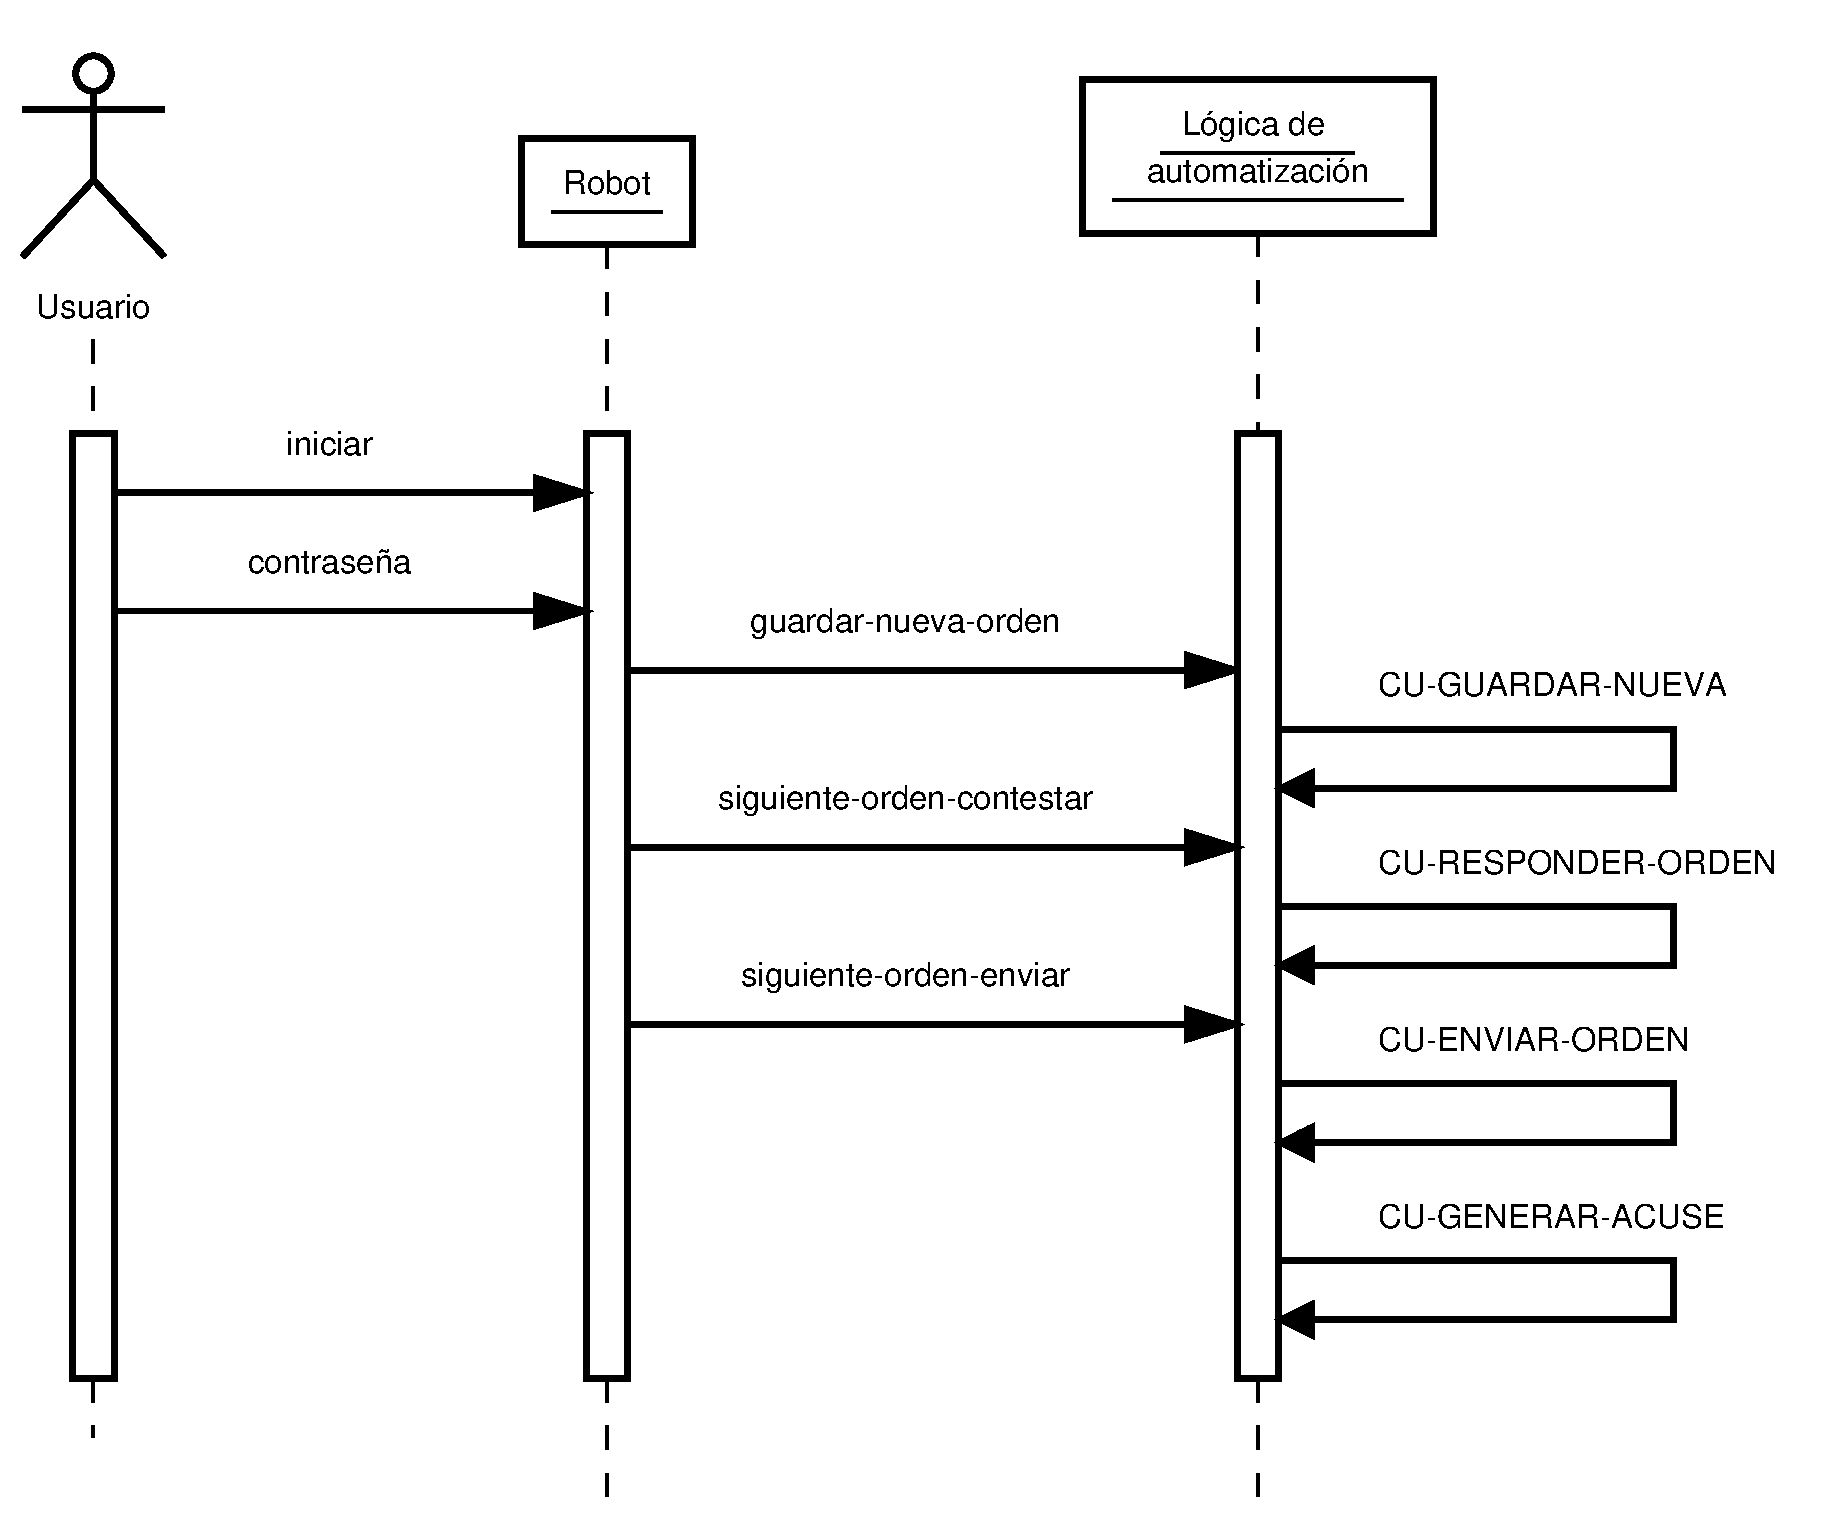
\includegraphics[scale=0.7]{dia-seq-cu-contestar}
	\caption{Diagrama de secuencia del caso de uso CU-CONTESTAR.}
	\label{fig:dia-seq-cu-contestar}
\end{figure}

\subsubsection{Guardar nueva orden}
El diseño para la solución del caso de uso \textbf{CU-GUARDAR-NUEVA} (sección \ref{cu-guardar-nueva}) utiliza los componentes \textbf{Agente}, \textbf{Lógica de Automatización} y \textbf{Persistencia}, tal solución se logra realizando las siguientes llamadas (en el diagrama de la Figura \ref{fig:dia-seq-cu-guardar-nueva} se muestra el diagrama de secuencia.):
\begin{enumerate}
	\item \textbf{Agente}: envía los datos de la nueva orden de reposición (mensaje 1 del diagrama).
	\item \textbf{Lógica de Automatización}: remueve (de encontrarse) los espacios en blanco al principio y al final de cada dato de la orden.
	\item \textbf{Lógica de Automatización}: construye la \textit{URL} de envío de la orden de reposición.
	\item \textbf{Lógica de Automatización}: envía la orden de reposición al componente de persistencia, (mensaje 2 del diagrama).
	\item \textbf{Persistencia}: almacena la orden de reposición en la base de datos.
\end{enumerate}

\begin{figure}[h]
	\centering
	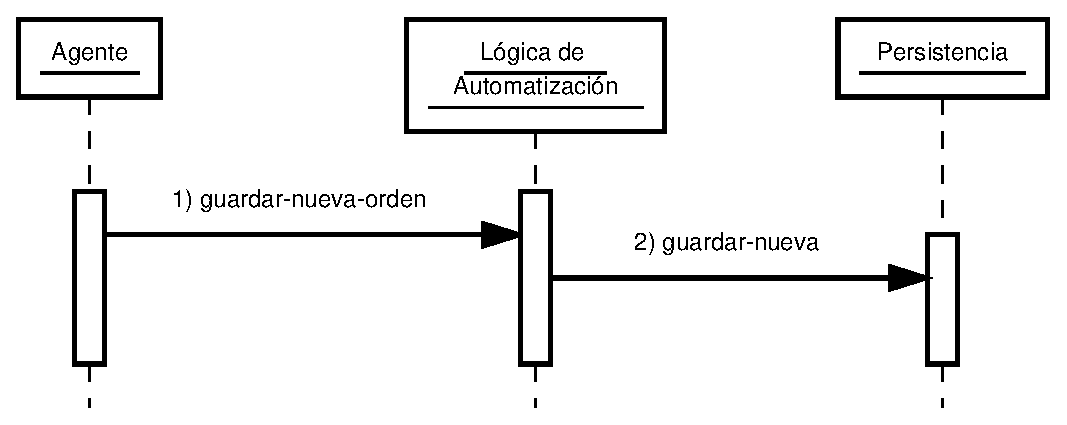
\includegraphics[scale=0.7]{dia-seq-cu-guardar-nueva}
	\caption{Diagrama de secuencia del caso de uso CU-GUARDAR-NUEVA.}
	\label{fig:dia-seq-cu-guardar-nueva}
\end{figure}

\subsubsection{Responder orden}
El diseño para la solución del caso de uso \textbf{CU-RESPONDER-ORDEN} (sección \ref{cu-responder-orden}) utiliza los componentes \textbf{Agente}, \textbf{Lógica de Automatización} y \textbf{Persistencia}, tal solución se logra realizando las siguientes llamadas (en el diagrama de la Figura \ref{fig:dia-seq-cu-responder-orden} se muestra el diagrama de secuencia):
\begin{enumerate}
	\item \textbf{Agente}: pide la siguiente orden de reposición para contestar (mensaje 1 del diagrama).
	\item \textbf{Lógica de Automatización}: consulta el componente \textbf{Persistencia} para obtener la siguiente orden para contestar.
	\item \textbf{Persistencia}: obtiene la primera orden de reposición con estado de \textbf{Nueva}.
	\item \textbf{Persistencia}: cambia el estado de la orden a \textbf{Siendo Contestada} (mensaje 3 del diagrama).
	\item \textbf{Agente}: pide los datos para llenar los formularios (mensaje 6 del diagrama).
	\item \textbf{Agente}: pide almacenar los datos de la orden de reposición contestada (mensaje 7 del diagrama).
	\item \textbf{Lógica de Automatización}: envía los datos de la orden contestada al componente \textbf{Persistencia} para que sean almacenados (mensaje 8 del diagrama).
	\item \textbf{Lógica de Automatización}: manda el cambio de estado de la orden a \textbf{Contestada} (mensaje 9 del diagrama).
\end{enumerate}

\begin{figure}[h]
	\centering
	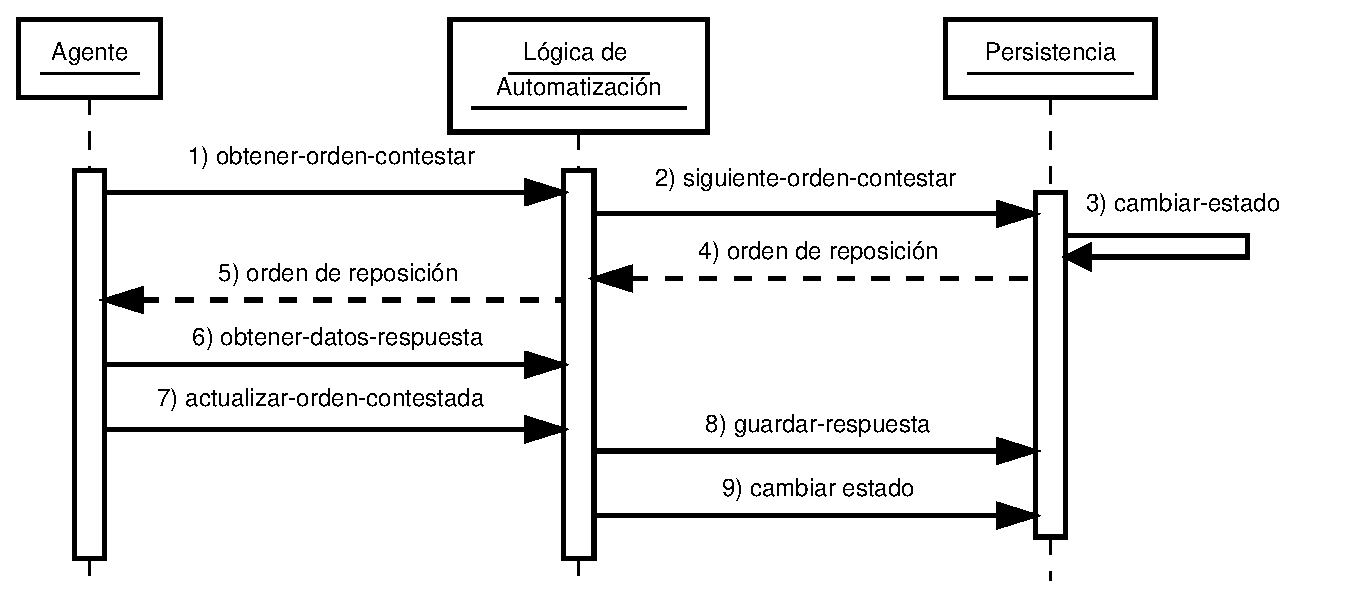
\includegraphics[scale=0.7]{dia-seq-cu-responder-orden}
	\caption{Diagrama de secuencia del caso de uso CU-RESPONDER-ORDEN.}
	\label{fig:dia-seq-cu-responder-orden}
\end{figure}

\subsubsection{Enviar orden}
El diseño para la solución del caso de uso \textbf{CU-ENVIAR-ORDEN} (sección \ref{cu-enviar-orden}) utiliza los componentes \textbf{Agente}, \textbf{Lógica de Automatización} y \textbf{Persistencia}, tal solución se logra realizando las siguientes llamadas (en el diagrama de la Figura \ref{fig:dia-seq-cu-enviar-orden} se muestra el diagrama de secuencia):
\begin{enumerate}
	\item \textbf{Agente}: pide la siguiente orden de reposición para enviar (mensaje 1 del diagrama).
	\item \textbf{Lógica de Automatización}: consulta el componente \textbf{Persistencia} para obtener la siguiente orden para enviar (mensaje 2 del diagrama).
	\item \textbf{Persistencia}: obtiene la primera orden de reposición con estado de \textbf{Contestada}.
	\item \textbf{Persistencia}: cambia el estado de la orden a \textbf{Siendo Enviada} (mensaje 3 del diagrama).
	\item \textbf{Agente}: dirige el explorador a la \textit{URL de envío}.
	\item \textbf{Agente}: manda almacenar el folio de envío (mensaje 6 del diagrama).
	\item \textbf{Lógica de Automatización}: utiliza el componente \textbf{Persistencia} para almacenar el folio de envío (mensaje 7 del diagrama).
	\item \textbf{Lógica de Automatización}: actualiza el estado de la orden a \textbf{Enviada} (mensaje 8 del diagrama).
\end{enumerate}

\begin{figure}[h]
	\centering
	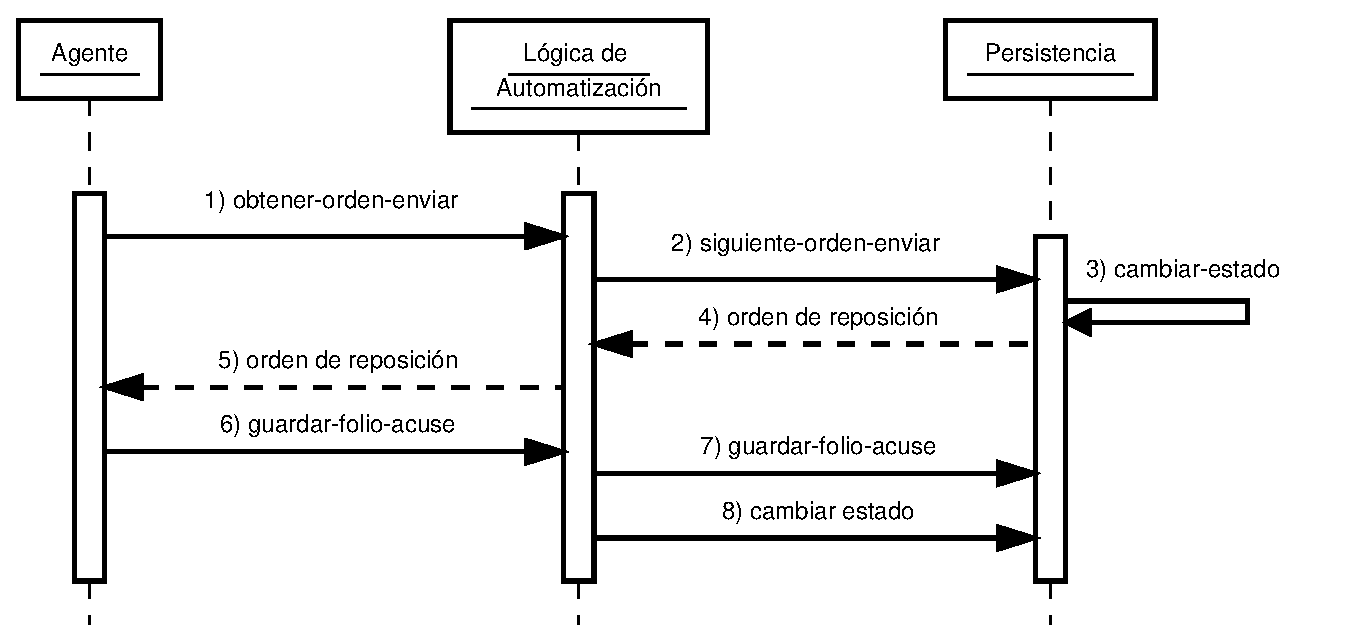
\includegraphics[scale=0.7]{dia-seq-cu-enviar-orden}
	\caption{Diagrama de secuencia del caso de uso CU-ENVIAR-ORDEN.}
	\label{fig:dia-seq-cu-enviar-orden}
\end{figure}

\subsubsection{Generar acuse de envío}
El diseño para la solución del caso de uso \textbf{CU-GENERAR-ACUSE} (sección \ref{cu-generar-acuse}) utiliza los componentes \textbf{Lógica de Automatización}, \textbf{Persistencia}, \textbf{Generador de Reportes} y \textbf{Sistema de Archivos} tal solución se logra realizando las siguientes llamadas (en el diagrama de la Figura \ref{fig:dia-seq-cu-generar-acuse} se muestra el diagrama de secuencia):
\begin{enumerate}
	\item \textbf{Lógica de Automatización}: pide los datos de la orden de reposición al componente \textbf{Persistencia} (mensaje 1 del diagrama).
	\item \textbf{Lógica de Automatización}: pide la generación del acuse de envío al componente \textbf{Generador de Reportes} (mensaje 2 del diagrama).
	\item \textbf{Generador de Reportes}: pide almacenar el acuse de envío al componente \textbf{Sistema de Archivos} (mensaje 3 del diagrama).
\end{enumerate}

\begin{figure}[h]
	\centering
	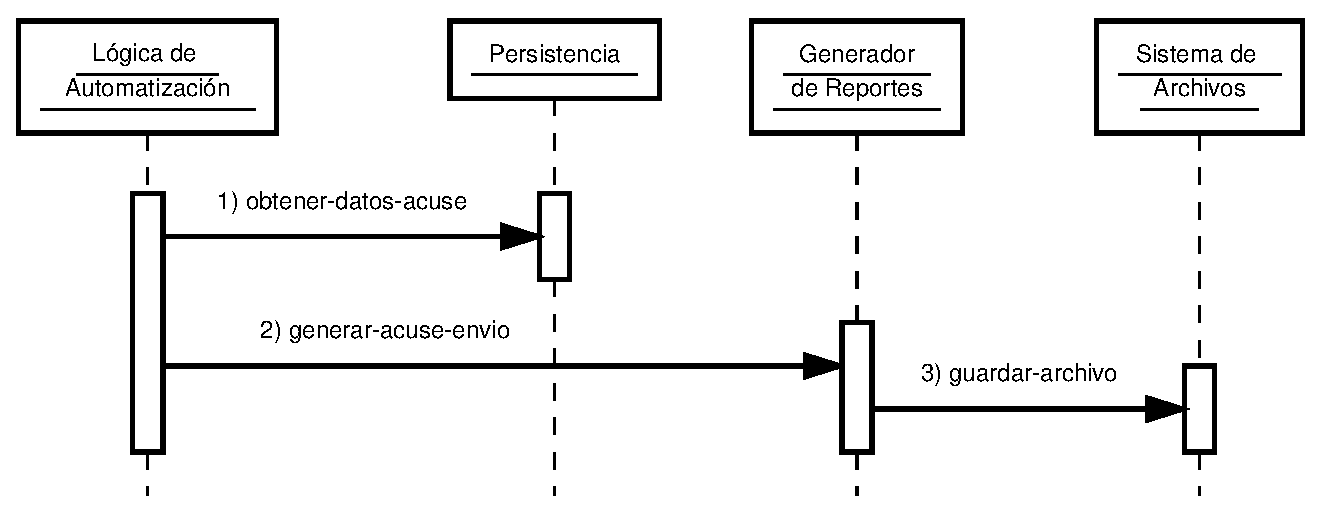
\includegraphics[scale=0.7]{dia-seq-cu-generar-acuse}
	\caption{Diagrama de secuencia del caso de uso CU-GENERAR-ACUSE.}
	\label{fig:dia-seq-cu-generar-acuse}
\end{figure}

\subsubsection{Verificar órdenes}
El diseño de la solución al caso de uso \textbf{CU-VERIFICAR} (sección \ref{cu-verificar}) se lleva a cabo entre el actor \textbf{Usuario} y los componentes \textbf{Agente} \textbf{Lógica de Automatización} tal solución se logra realizando las siguientes llamadas (en el diagrama de la Figura \ref{fig:dia-seq-cu-verificar} se muestra el diagrama de secuencia):
\begin{enumerate}
	\item \textbf{Usuario}: inicia la ejecución del agente (mensaje 1 del diagrama).
	\item \textbf{Agente}: dirige el explorador de Internet a la página del Sistema de Abastecimiento y pide al usuario la contraseña para ingresar.
	\item \textbf{Usuario}: proporciona la contraseña (mensaje 2 del diagrama).
	\item \textbf{Agente}: realiza el acceso al Sistema de Abastecimiento.
	\item \textbf{Agente}: dirige el explorador de Internet a la búsqueda de órdenes de reposición.
	\item \textbf{Agente}: pide el rango de fechas al componente \textbf{Lógica de Automatización} (mensaje 3 del diagrama).
	\item \textbf{Agente}: realiza la búsqueda de órdenes de reposición \textit{canceladas}.
	\item \textbf{Agente}: envía el listado con los números de orden de reposición resultantes al componente \textbf{Lógica de Automatización} (mensaje 4 del diagrama).
	\item \textbf{Lógica de Automatización}: ejecuta los casos de uso \textbf{CU-ACTUALIZAR-ESTATUS-SA} (mensaje 5 del diagrama).
\end{enumerate}

\begin{figure}[h]
	\centering
	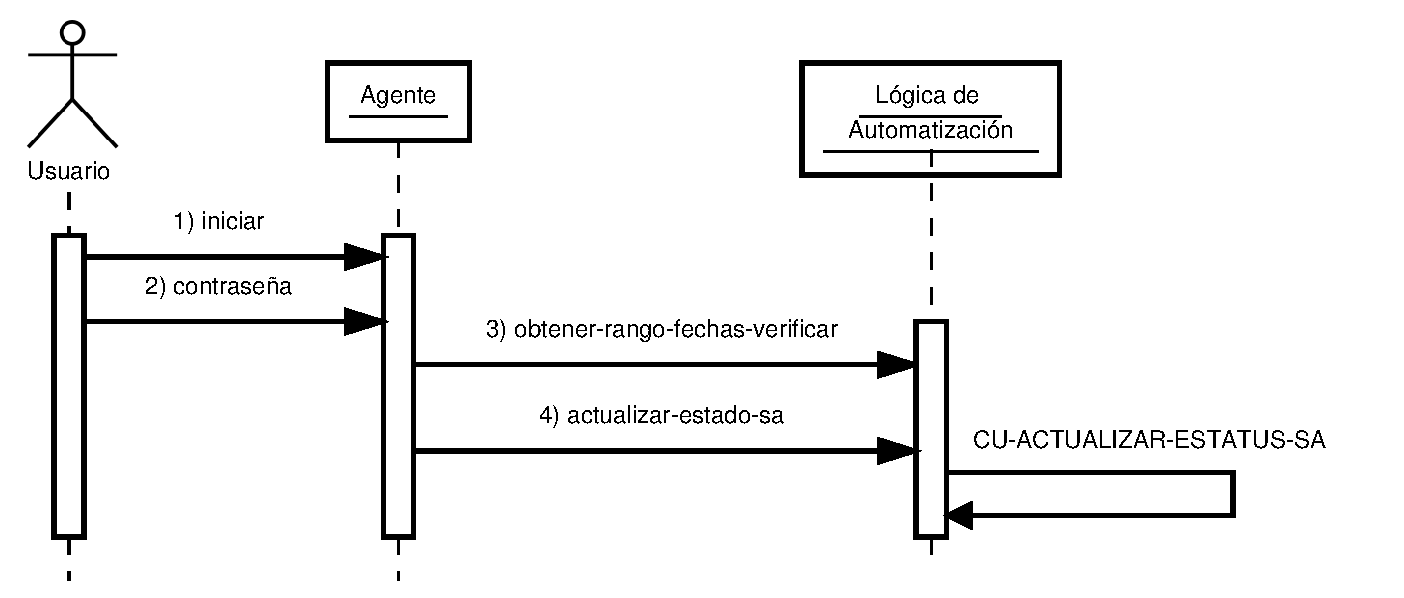
\includegraphics[scale=0.7]{dia-seq-cu-verificar}
	\caption{Diagrama de secuencia del caso de uso CU-VERIFICAR.}
	\label{fig:dia-seq-cu-verificar}
\end{figure}

\subsubsection{Actualizar estatus de Sistema de Abastecimiento}
El diseño para la solución del caso de uso \textbf{CU-ACTUALIZAR-ESTATUS-SA} (sección \ref{cu-actualizar-estatus-sa}) utiliza los componentes \textbf{Agente}, \textbf{Lógica de Automatización} y \textbf{Persistencia}, tal solución se logra realizando las siguientes llamadas (en el diagrama de la Figura \ref{fig:dia-seq-cu-actualizar-estatus-sa} se muestra el diagrama de secuencia):
\begin{enumerate}
	\item \textbf{Lógica de Automatización}: envía el listado de con los números de órdenes de reposición al componente \textbf{Persistencia} para actualizar en la base de datos el estado conocido en el Sistema de Abastecimiento (mensaje 1 del diagrama).
\end{enumerate}

\begin{figure}[h]
	\centering
	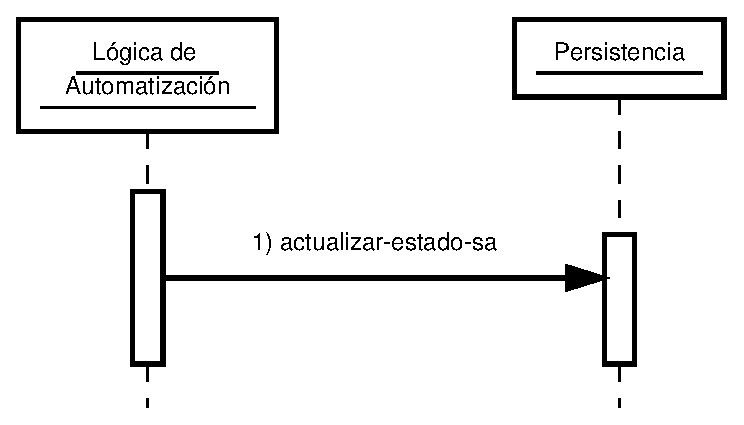
\includegraphics[scale=0.7]{dia-seq-cu-actualizar-estatus-sa}
	\caption{Diagrama de secuencia del caso de uso CU-ACTUALIZAR-ESTATUS-SA.}
	\label{fig:dia-seq-cu-actualizar-estatus-sa}
\end{figure}

\subsubsection{Entrar en interfaz Web}
El diseño de la solución al caso de uso \textbf{CU-ENTRAR-WEB} (sección \ref{cu-entrar-web}) se lleva a cabo entre el actor \textbf{Usuario} y los componentes \textbf{Portal Web} y \textbf{Persistencia} tal solución se logra realizando las siguientes llamadas (en el diagrama de la Figura \ref{fig:dia-seq-cu-entrar-web} se muestra el diagrama de secuencia):
\begin{enumerate}
	\item \textbf{Usuario}: introduce su nombre de usuario y contraseña \textbf{credenciales} (mensaje 1 del diagrama).
	\item \textbf{Portal Web}: envía el nombre de usuario al componente \textbf{Persistencia} que realiza la búsqueda de los datos del usuario (mensaje 2 del diagrama).
	\item \textbf{Portal Web}: compara la contraseña con la almacenada en la base de datos.
	\begin{enumerate}
		\item \textit{Si las credenciales son válidas}: el \textbf{Portal Web}regresa al \textbf{Usuario} un código de acceso temporal (mensaje 3 del diagrama).
		\item \textit{Si las credenciales son inválidas}: el \textbf{Portal Web}regresa al \textbf{Usuario} un mensaje de error (mensaje 4 del diagrama).
	\end{enumerate}
\end{enumerate}

\begin{figure}[h]
	\centering
	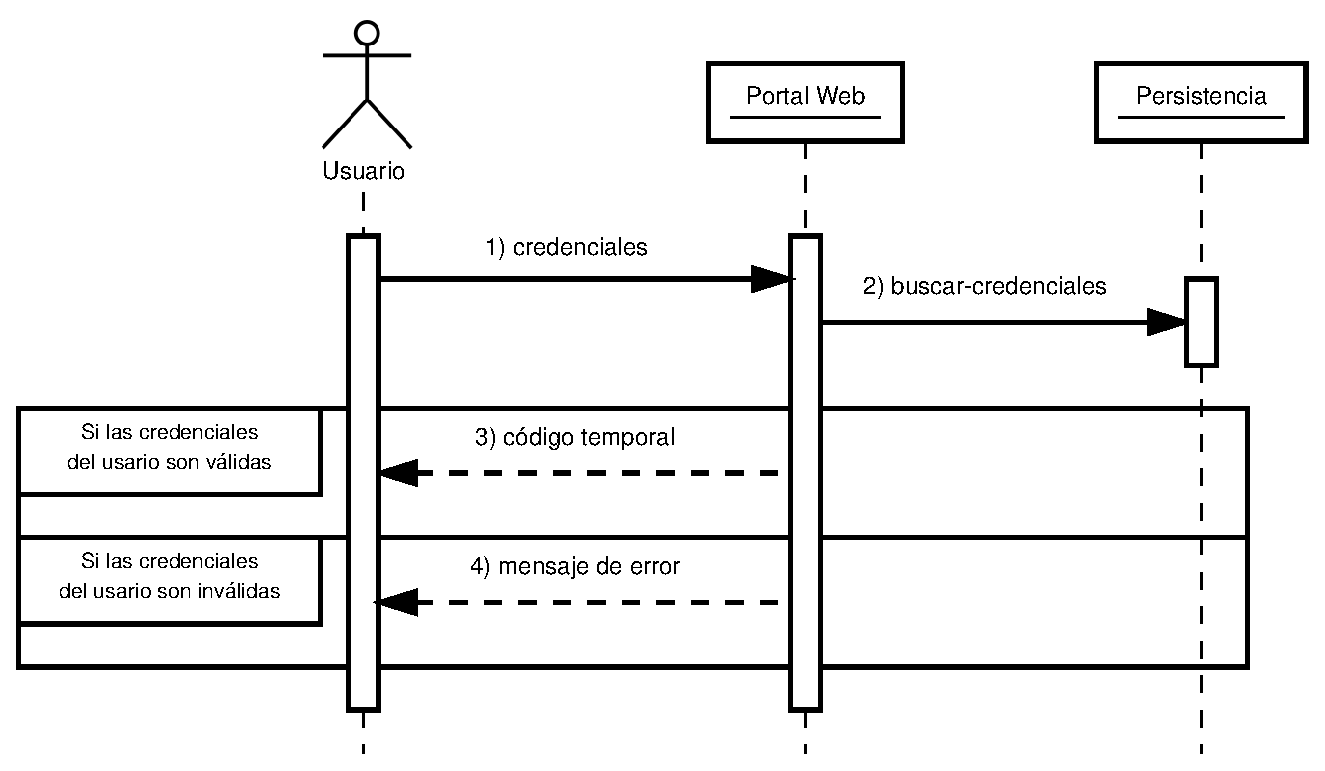
\includegraphics[scale=0.7]{dia-seq-cu-entrar-web}
	\caption{Diagrama de secuencia del caso de uso CU-ENTRAR-WEB.}
	\label{fig:dia-seq-cu-entrar-web}
\end{figure}

\subsubsection{Generar reporte}
El diseño de la solución al caso de uso \textbf{CU-GENERAR-REPORTE} (sección \ref{cu-generar-reporte}) se lleva a cabo entre el actor \textbf{Usuario} y los componentes \textbf{Portal Web}, \textbf{Persistencia}, \textbf{Generador de Reportes} y  \textbf{Sistema de Archivos} tal solución se logra realizando las siguientes llamadas (en el diagrama de la Figura \ref{fig:dia-seq-cu-generar-reporte} se muestra el diagrama de secuencia):
\begin{enumerate}
	\item \textbf{Usuario}: selecciona el tipo de reporte y el rango de fechas (mensaje 1 del diagrama).
	\item \textbf{Portal Web}: pide la búsqueda de órdenes al componente \textbf{Persistencia} (mensaje 2 del diagrama).
	\item \textbf{Portal Web}: envía las órdenes para generar el reporte (mensaje 3 del diagrama).
	\item \textbf{Generador de Reportes}: genera el reporte.
	\item \textbf{Generador de Reportes}: pide al componente \textbf{Sistema de Archivos} almacenar el reporte (mensaje 4 del diagrama).
	\item \textbf{Generador de Reportes}: regresa la ruta donde se guardó el componente (mensaje 5 del diagrama).
	\item \textbf{Portal Web}: muestra al \textbf{Usuario} la ruta donde se encuentra el reporte (mensaje 6 del diagrama).
\end{enumerate}

\begin{figure}[h]
	\centering
	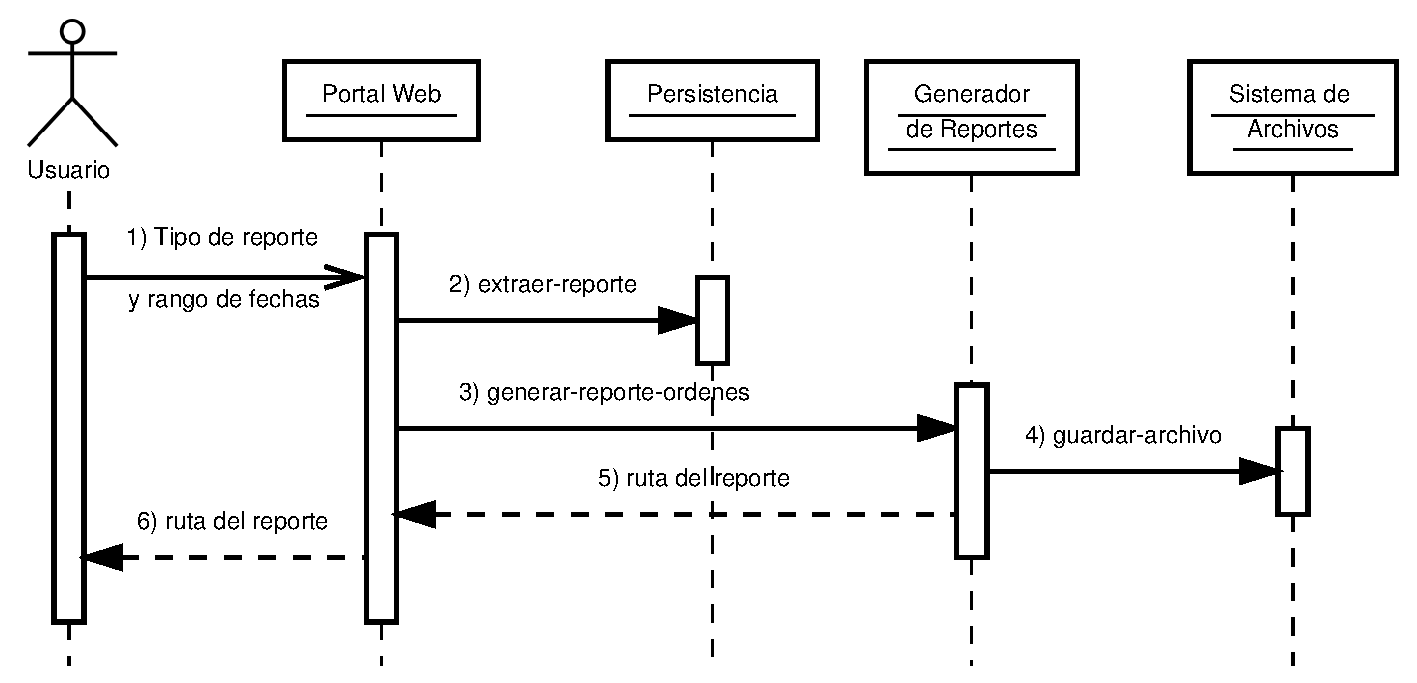
\includegraphics[scale=0.7]{dia-seq-cu-generar-reporte}
	\caption{Diagrama de secuencia del caso de uso CU-GENERAR-REPORTE.}
	\label{fig:dia-seq-cu-generar-reporte}
\end{figure}

\subsubsection{Actualizar catálogo}
El diseño de la solución al caso de uso \textbf{CU-ACTUALIZAR-CATALOGO} (sección \ref{cu-actualizar-catalogo}) se lleva a cabo entre el actor \textbf{Usuario} y los componentes \textbf{Portal Web} y \textbf{Persistencia} tal solución se logra realizando las siguientes llamadas (en el diagrama de la Figura \ref{fig:dia-seq-cu-actualizar-catalogo} se muestra el diagrama de secuencia):
\begin{enumerate}
	\item \textbf{Usuario}: selecciona el catálogo y el archivo (mensaje 1 del diagrama).
	\item \textbf{Portal Web}: pide la actualización del catálogo al componente \textbf{Persistencia} (mensaje 2 del diagrama).
	\item \textbf{Portal Web}: muestra al \textbf{Usuario} la cantidad de registros almacenados (mensaje 3 del diagrama).
\end{enumerate}

\begin{figure}[h]
	\centering
	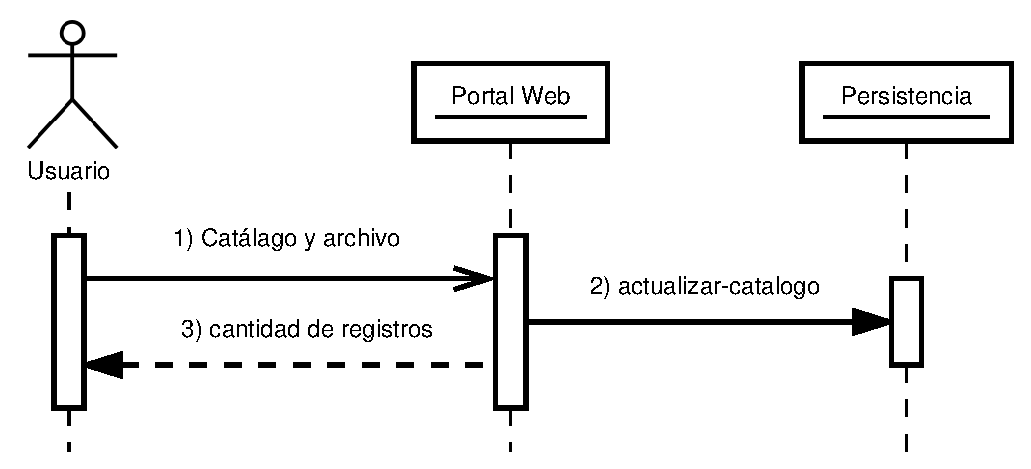
\includegraphics[scale=0.7]{dia-seq-cu-actualizar-catalogo}
	\caption{Diagrama de secuencia del caso de uso CU-ACTUALIZAR-CATALOGO.}
	\label{fig:dia-seq-cu-actualizar-catalogo}
\end{figure}

\subsubsection{Buscar órdenes}
El diseño de la solución al caso de uso \textbf{CU-BUSCAR} (sección \ref{cu-buscar}) se lleva a cabo entre el actor \textbf{Usuario} y los componentes \textbf{Portal Web} y \textbf{Persistencia} tal solución se logra realizando las siguientes llamadas (en el diagrama de la Figura \ref{fig:dia-seq-cu-buscar} se muestra el diagrama de secuencia):
\begin{enumerate}
	\item \textbf{Usuario}: llenada el formulario de búsqueda \textbf{filtro} (mensaje 1 del diagrama).
	\item \textbf{Portal Web}: pide la realización de la búsqueda de órdenes al componente \textbf{Persistencia} (mensaje 2 del diagrama).
	\item \textbf{Portal Web}: muestra al \textbf{Usuario} el listado de órdenes de reposición encontradas (mensaje 3 del diagrama).
\end{enumerate}

\begin{figure}[h]
	\centering
	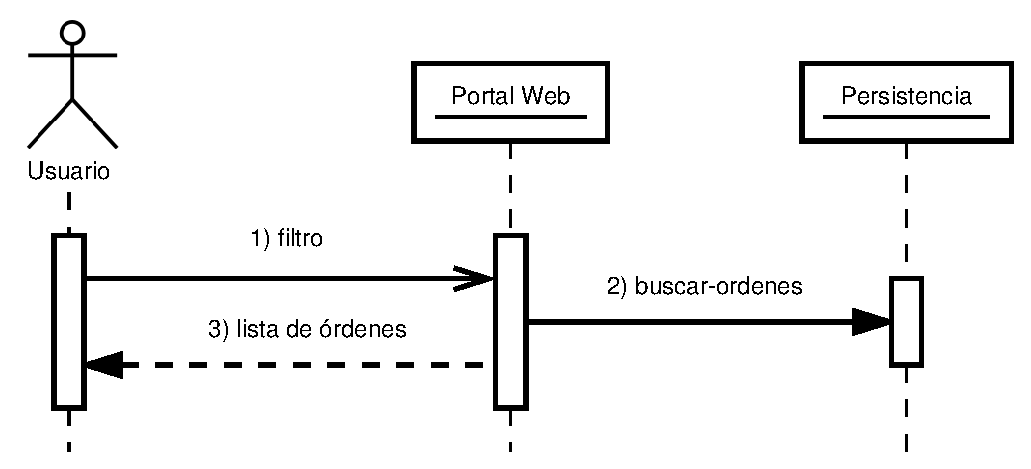
\includegraphics[scale=0.7]{dia-seq-cu-buscar}
	\caption{Diagrama de secuencia del caso de uso CU-BUSCAR.}
	\label{fig:dia-seq-cu-buscar}
\end{figure}

\subsubsection{Visualizar orden}
El diseño de la solución al caso de uso \textbf{CU-VISUALIZAR} (sección \ref{cu-visualizar}) se lleva a cabo entre el actor \textbf{Usuario} y los componentes \textbf{Portal Web} y \textbf{Persistencia} tal solución se logra realizando las siguientes llamadas (en el diagrama de la Figura \ref{fig:dia-seq-cu-visualizar} se muestra el diagrama de secuencia):
\begin{enumerate}
	\item \textbf{Usuario}: selecciona la orden de reposición (mensaje 1 del diagrama).
	\item \textbf{Portal Web}: pide la realización de la búsqueda de la orden al componente \textbf{Persistencia} (mensaje 2 del diagrama).
	\item \textbf{Portal Web}: muestra al \textbf{Usuario} la información de la orden de reposición.
\end{enumerate}

\begin{figure}[h]
	\centering
	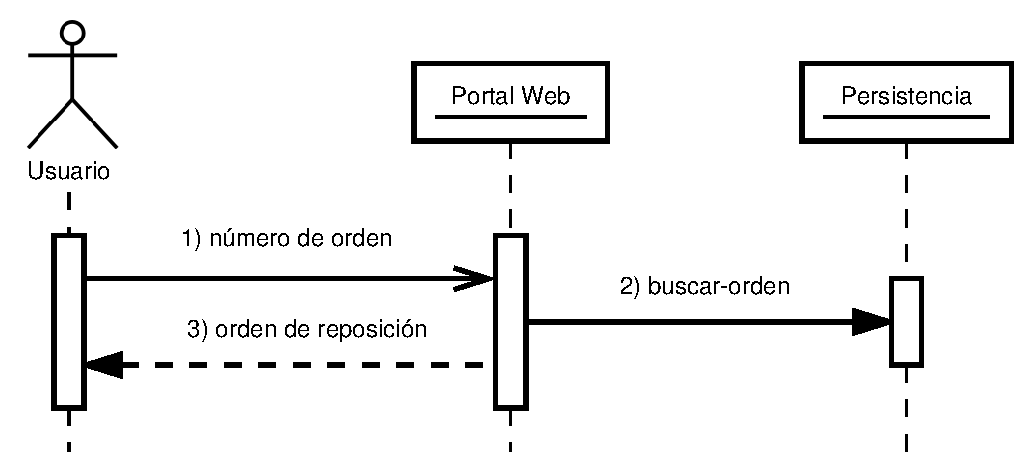
\includegraphics[scale=0.7]{dia-seq-cu-visualizar}
	\caption{Diagrama de secuencia del caso de uso CU-VISUALIZAR.}
	\label{fig:dia-seq-cu-visualizar}
\end{figure}

\subsubsection{Editar orden}
Ver sección \ref{cu-contestar}.\\
El diseño de la solución al caso de uso \textbf{CU-EDITAR} (sección \ref{cu-editar}) se lleva a cabo entre el actor \textbf{Usuario} y los componentes \textbf{Portal Web} y \textbf{Persistencia} tal solución se logra realizando las siguientes llamadas (en el diagrama de la Figura \ref{fig:dia-seq-cu-editar} se muestra el diagrama de secuencia):
\begin{enumerate}
	\item \textbf{Usuario}: activa la edición de la orden de reposición (mensaje 1 del diagrama).
	\item \textbf{Usuario}: modifica la información de la orden de reposición (mensaje 2).
	\item \textbf{Portal Web}: pide la actualización de la orden al componente \textbf{Persistencia} (mensaje 3 del diagrama).
\end{enumerate}

\begin{figure}[h]
	\centering
	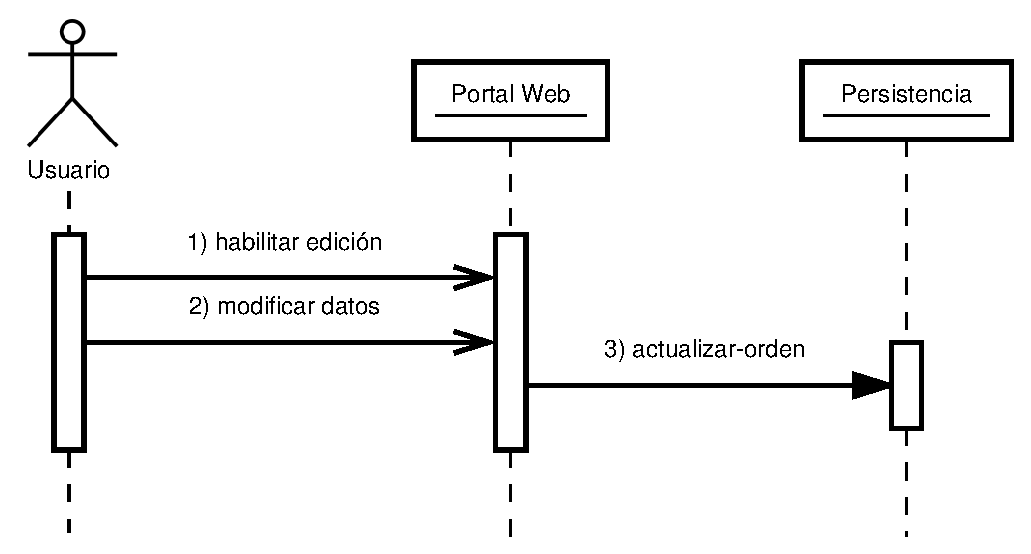
\includegraphics[scale=0.7]{dia-seq-cu-editar}
	\caption{Diagrama de secuencia del caso de uso CU-EDITAR.}
	\label{fig:dia-seq-cu-editar}
\end{figure}


%===============================================================================
%===============================================================================

\newpage
\section{Diseño de la base de datos}
La base de datos tiene dos finalidades, guardar la información capturada de las órdenes de reposición atendidas así como los catálogos necesarios para los procesos automatizados y generación de reportes; la segunda es almacenar la información de los usuarios autorizados para utilizar el portal web.\\
El diseño de la base de datos se centra en los siguientes grupos\footnote{Los nombres de las tablas están escritos utilizando letras minúsculas de alfabeto inglés y guión bajo $([a-z]{\_})^+$.}(ver Figura \ref{fig:dia-er-resumen}):
\begin{enumerate}
	\item Tablas de las órdenes de reposición.
	\item Tablas del registro de eventos.
	\item Tablas de los usuarios de la interfaz web.
	\item Catálogos para generación de reportes.
\end{enumerate}
\begin{figure}[h]
  \centering
  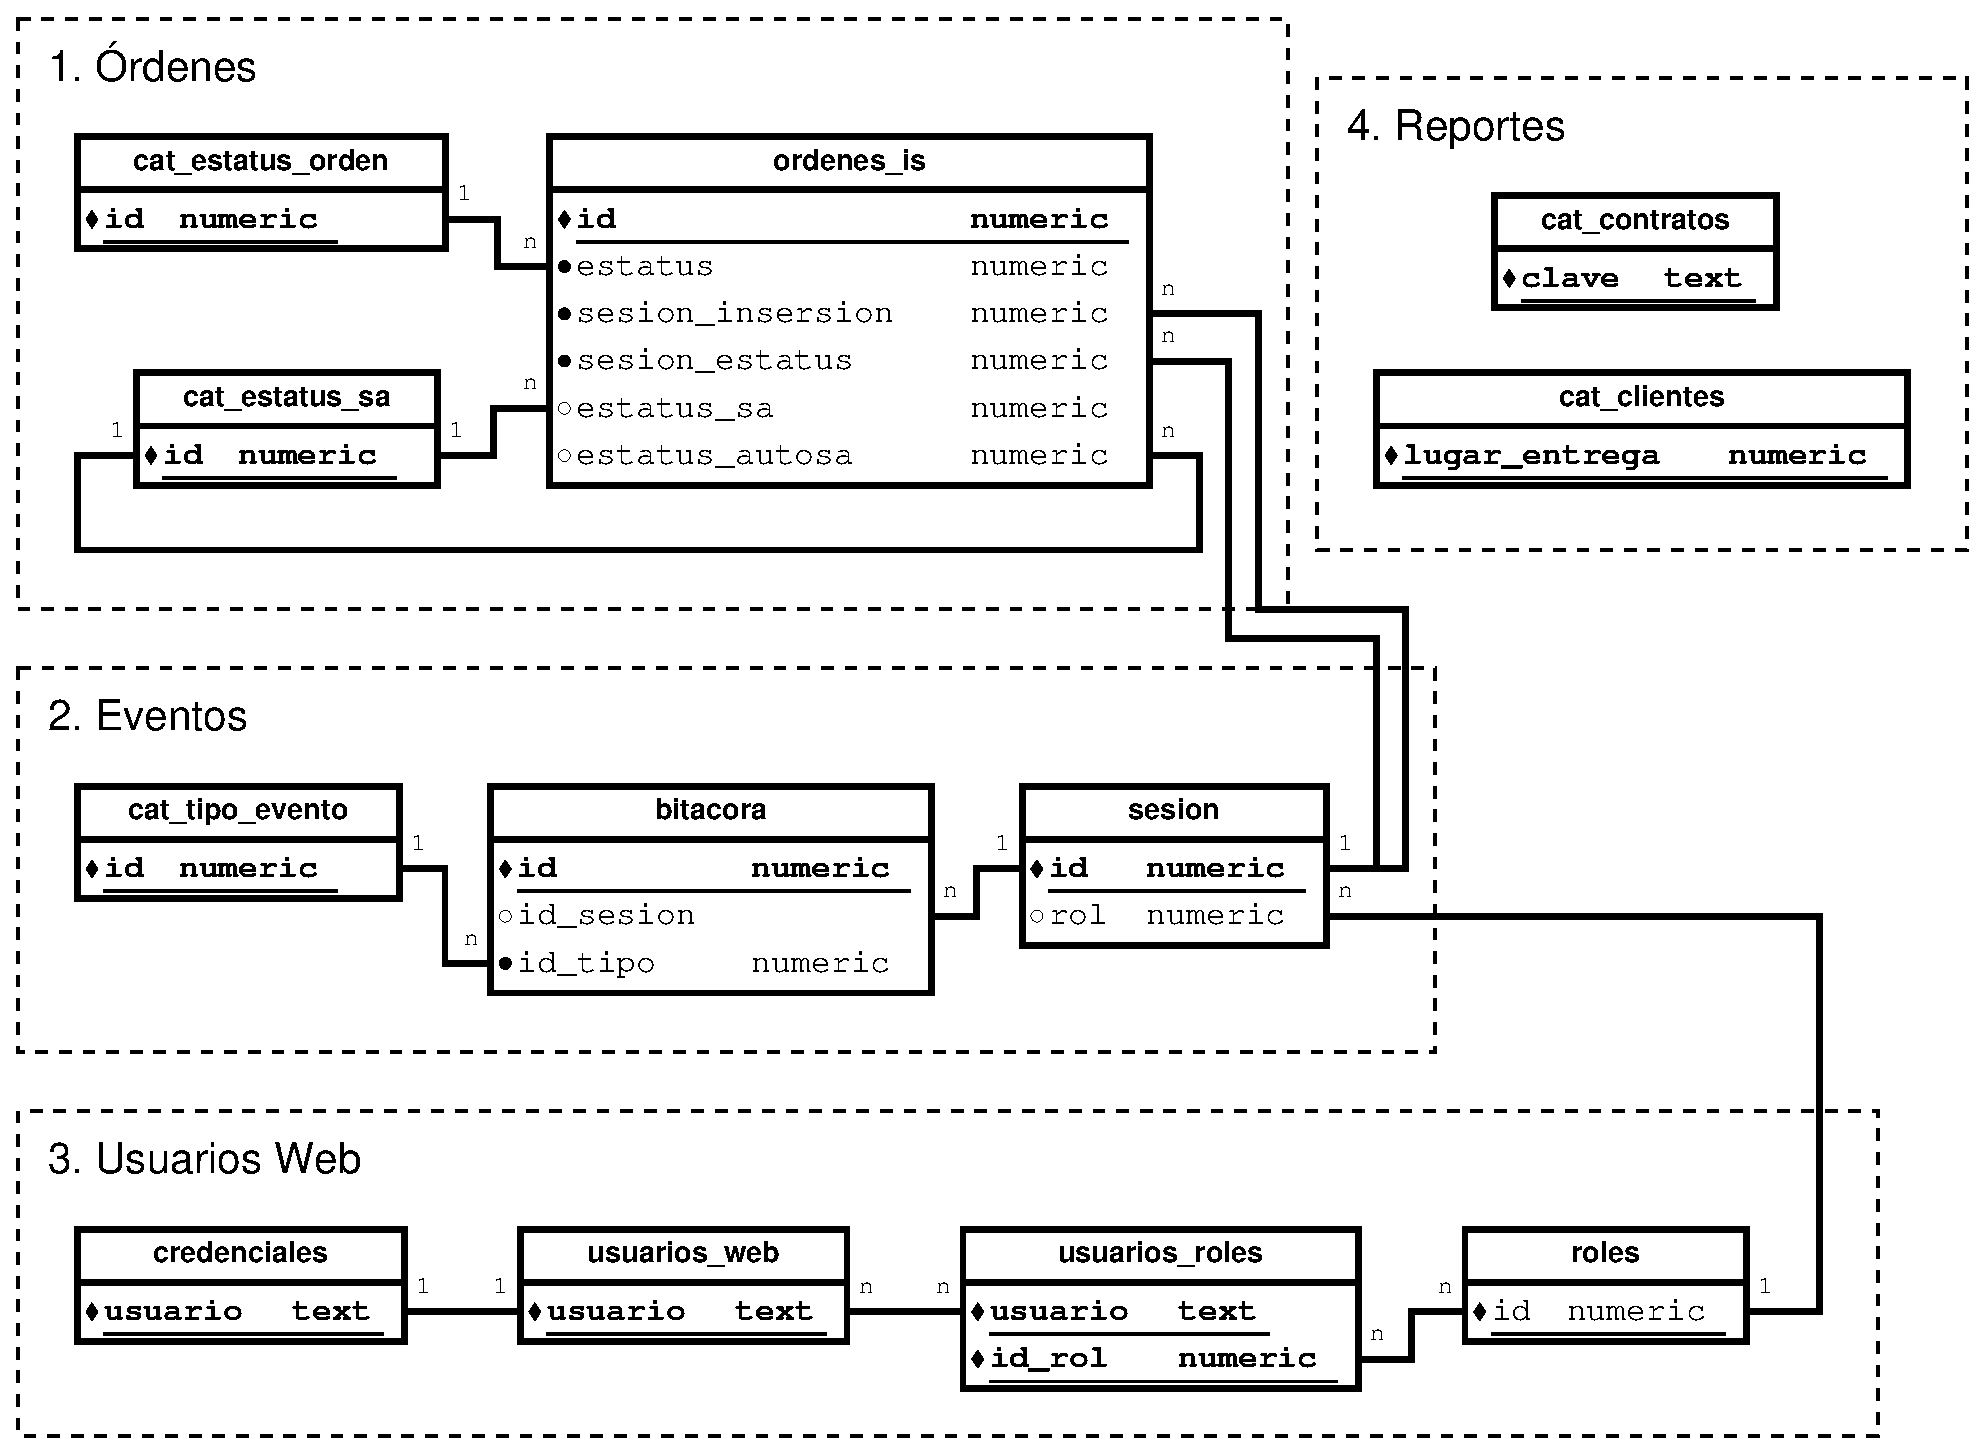
\includegraphics[width=\textwidth]{dia-er-resumen}
  \caption{Diagrama Entidad Relación de el Sistema AutoSA.}
  \label{fig:dia-er-resumen}
\end{figure}


\subsection{Tablas de las órdenes de reposición}
En estas tablas (ver Figura \ref{fig:dia-er-ordenes}) se almacenan las órdenes de reposición atendidas durante la rutina automatizada para responder órdenes de reposición en el Sistema de Abastecimiento\footnote{Ver caso de uso \ref{cu-contestar}.}, de igual manera también es utilizada en la verificación de órdenes de reposición canceladas\footnote{Ver caso de uso \ref{cu-verificar}.}.
\begin{figure}[h]
  \centering
  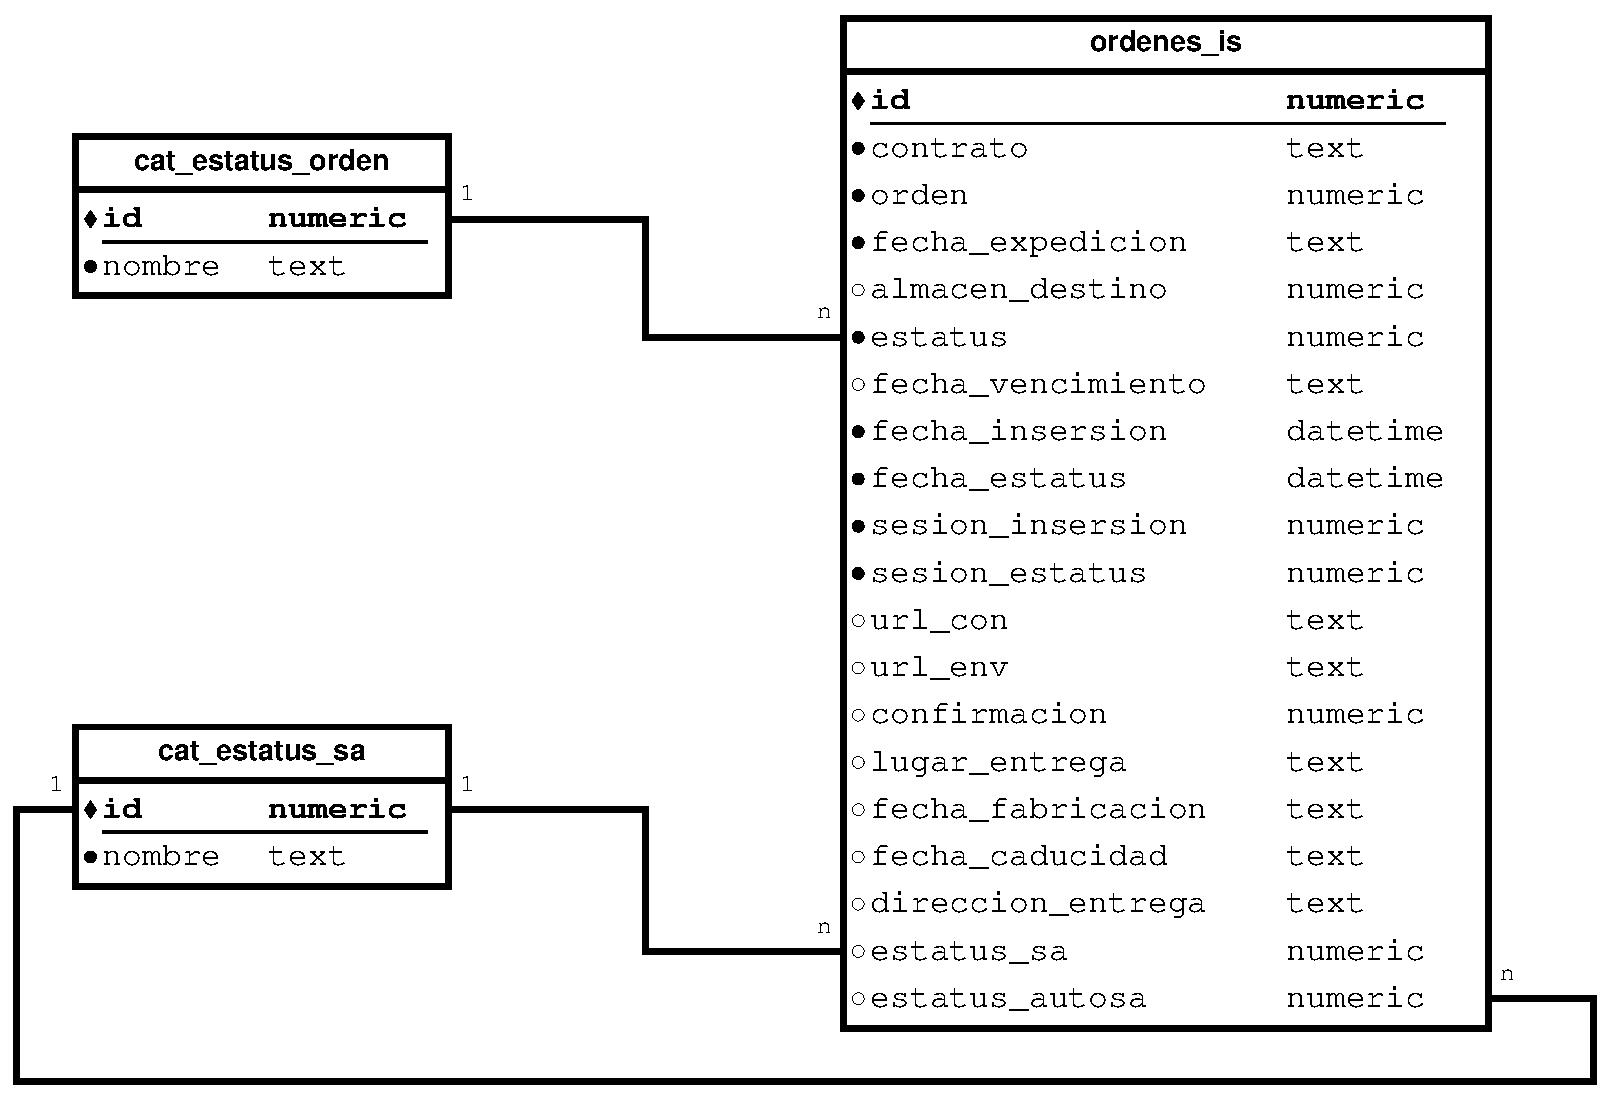
\includegraphics[scale=0.5]{dia-er-ordenes} 
  \caption{Diagrama Entidad Relación para el registro de órdenes de reposición.}
  \label{fig:dia-er-ordenes}
\end{figure}
\paragraph{ordenes{\textunderscore}is:} Contiene el registro de las órdenes de reposición del Sistema de Abastecimiento que han sido atendidas por la rutina de automatización.
\paragraph{cat{\textunderscore}estatus{\textunderscore}orden:} Este catálogo no debe ser alterado, contiene los posibles estatus que pude tomar una orden durante el ciclo de vida de la aplicación.
\paragraph{cat{\textunderscore}estatus{\textunderscore}sa:} Este catálogo contiene los estados definidos por el Sistema de Abastecimiento para registrar y almacenar una orden de reposición.


\subsection{Tablas del registro de eventos}
El registro de eventos es todo lo relacionado con actividad de los actores del sistema (agentes de automatización y usuarios), como se muestra en la Figura \ref{fig:dia-er-bitacora}.
\begin{figure}[h]
  \centering
  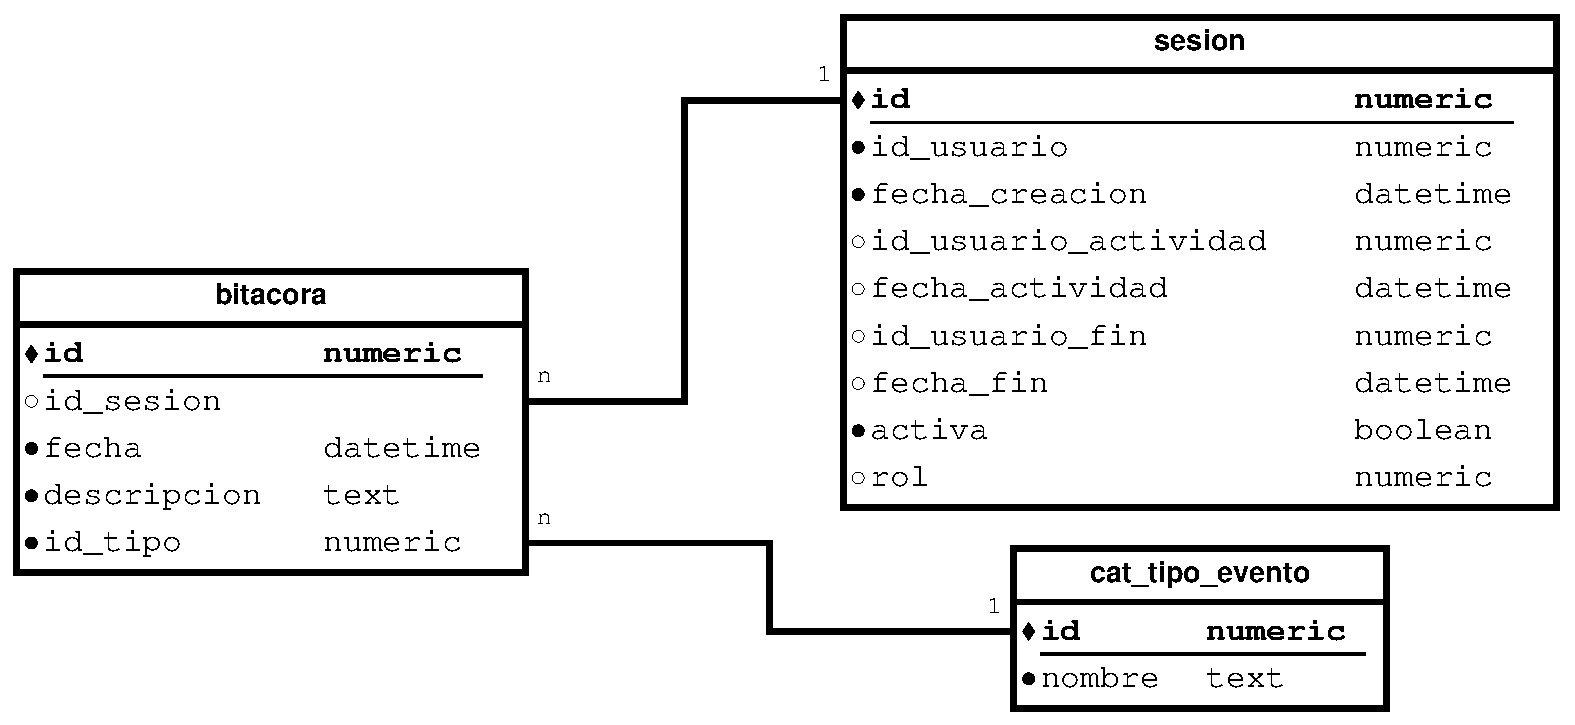
\includegraphics[scale=0.5]{dia-er-bitacora} 
  \caption{Diagrama Entidad Relación para el registro de eventos.}
  \label{fig:dia-er-bitacora}
\end{figure}
\paragraph{bitacora:} Lleva el registro de eventos ocurridos durante la ejecución de las rutinas de automatización, el evento puede estar ligado a una sesión.
\paragraph{cat{\textunderscore}tipo{\textunderscore}evento:} Catálogo con los tipos de eventos que pueden ser registrados en la bitácora.
\paragraph{sesion:} Define una sesión bajo la cual se ejecuta una rutina de automatización, la sesión puede definir implícitamente un usuario y un rol.


\subsection{Tablas de los usuarios de la interfaz web}
Las tablas de este grupo son utilizadas para gestionar el acceso a la interfaz web\footnote{Ver caso de uso \ref{cu-entrar-web}.} (ver Figura \ref{fig:dia-er-web}).
\begin{figure}[h]
  \centering
  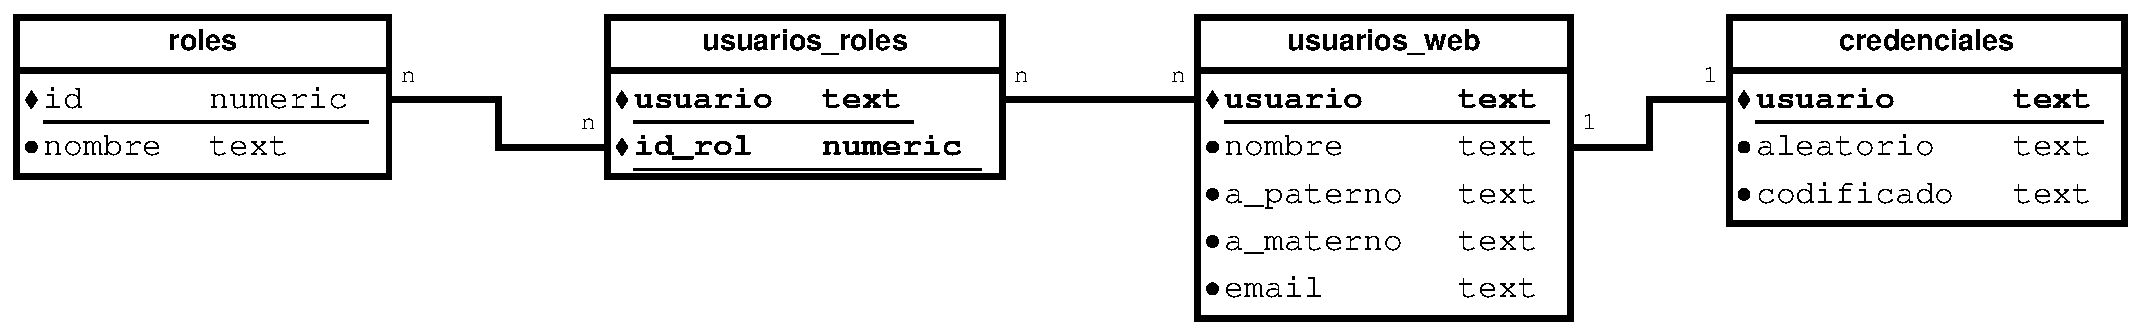
\includegraphics[scale=0.5]{dia-er-web} 
  \caption{Diagrama Entidad Relación para el manejo de usuarios.}
  \label{fig:dia-er-web}
\end{figure}
\paragraph{roles:}Contiene los roles (permisos) que los usuarios pueden tener en la interfaz web.
\paragraph{sesion:}Contiene información de las sesiones de los usuarios de la interfaz web.
\paragraph{usuarios{\textunderscore}web:} Contiene la información de los usuarios de la interfaz web.
\paragraph{credenciales:} Contiene la credenciales con las cuales los usuarios autentican su acceso a la interfaz web.


\subsection{Catálogos para la generación de reportes}
Estas tablas contienen catálogos (ver Figura \ref{fig:dia-er-reportes}) que son necesarios para la generación de los reportes\footnote{Ver casos de uso \ref{cu-generar-reporte} y \ref{cu-actualizar-catalogo}.} que sirven que las siguientes áreas de la farmacéutica continúen con la atención de las órdenes de reposición.
\begin{figure}[h]
  \centering
  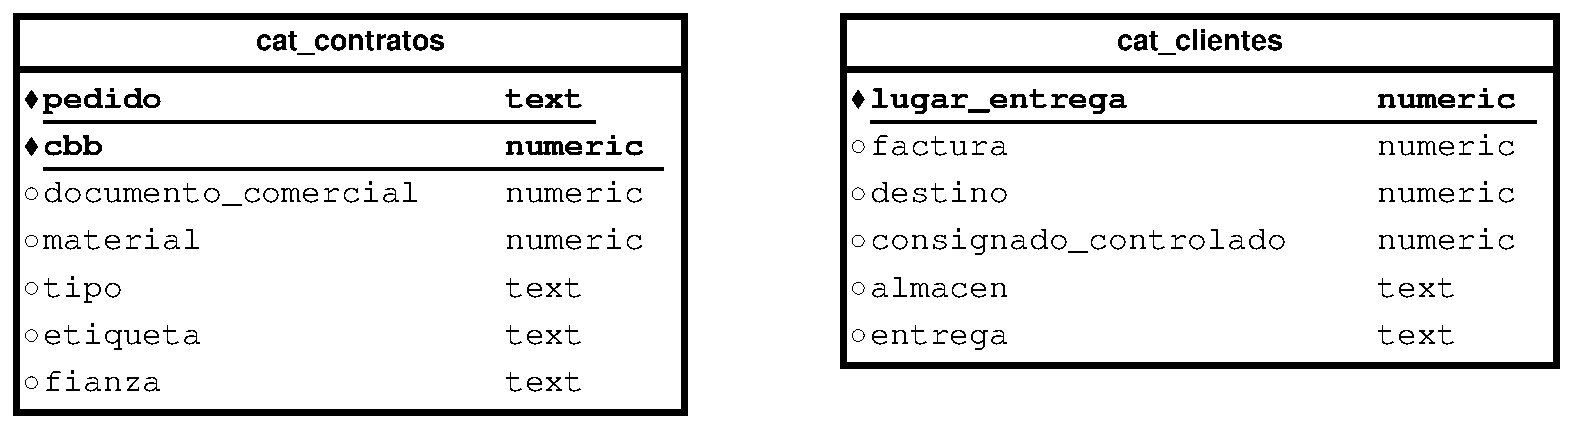
\includegraphics[scale=0.5]{dia-er-reportes} 
  \caption{Diagrama Entidad Relación de los catálogos para la generación de vistas.}
  \label{fig:dia-er-reportes}
\end{figure}
\paragraph{cat{\textunderscore}clientes:} Este catálogo contiene información sobre la localización física de los lugares donde deben ser entregados los productos.
\paragraph{cat{\textunderscore}contratos:} Este catálogo contiene información referente a acuerdos comerciales referentes a los productos requeridos en las órdenes de reposición.


\section{Resumen}
En este capítulo se ha mostrado la arquitectura del Sistema AutoSA, los componentes del mismo y las interfaces que ofrecen. Posteriormente se ha mostrado el flujo de mensajes entre los componentes del sistema para llevar a cabo los casos de uso del Capítulo \ref{cap2}. Así mismo se ha modelado la base de datos que a grandes rasgos está destinada a almacenar información de las órdenes de reposición e información de los usuarios del Sistema AutoSA.\\
El diseño planteado será implementado en el siguiente capítulo donde se verá a detalle el funcionamiento de cada módulo así como algoritmos, tecnologías y marcos de trabajo utilizados. 

%\nocite{*} 
% \bibliographystyle{unsrt}
\bibliographystyle{apacite}
\bibliography{bibliografia}
\end{document}